\documentclass[11pt]{article}
\usepackage[T1]{fontenc}
\usepackage{lmodern}
\usepackage{amsmath,amssymb,amsthm,mathtools,mathrsfs}
\usepackage[margin=1in]{geometry}
\usepackage{enumitem,microtype,booktabs,array,longtable}
\usepackage{xcolor,graphicx,tikz}
\usetikzlibrary{arrows.meta,positioning,calc,fit,decorations.pathreplacing,shapes.geometric}
\usepackage[hyphens]{url}
\usepackage[colorlinks=true,linkcolor=black,citecolor=blue!55!black,urlcolor=blue!55!black]{hyperref}
\usepackage[nameinlink,noabbrev,capitalize]{cleveref}
\hypersetup{pdftitle={The Poisson--Dirichlet law for prime predecessors},pdfauthor={OpenAI}}
\newcommand{\1}{\mathbf{1}}
\newcommand{\e}{\mathrm{e}}
\newcommand{\E}{\mathbb E}
\newcommand{\Prob}{\mathbb P}
\newcommand{\N}{\mathbb N}
\newcommand{\Z}{\mathbb Z}
\newcommand{\R}{\mathbb R}
\newcommand{\C}{\mathbb C}
\newcommand{\eps}{\varepsilon}
\newcommand{\dd}{\,\mathrm d}
\DeclarePairedDelimiter{\norm}{\lVert}{\rVert}
\DeclarePairedDelimiter{\abs}{\lvert}{\rvert}
\newcommand{\inner}[2]{\langle #1,#2\rangle}
\DeclareMathOperator{\Li}{Li}
\DeclareMathOperator{\supp}{supp}
\DeclareMathOperator{\cond}{cond}
\DeclareMathOperator{\lcm}{lcm}
\DeclareMathOperator{\rad}{rad}
\DeclareMathOperator{\PD}{PD}
\newtheorem{theorem}{Theorem}[section]
\newtheorem{lemma}[theorem]{Lemma}
\newtheorem{proposition}[theorem]{Proposition}
\newtheorem{corollary}[theorem]{Corollary}
\theoremstyle{definition}
\newtheorem{definition}[theorem]{Definition}
\theoremstyle{remark}
\newtheorem{remark}[theorem]{Remark}
\numberwithin{equation}{section}
\setlist[enumerate]{itemsep=3pt,topsep=5pt}
\setlist[itemize]{itemsep=3pt,topsep=5pt}
\allowdisplaybreaks[1]
\emergencystretch=1em

\title{The Poisson--Dirichlet law for prime predecessors}
\author{OpenAI}
\date{September 24, 2026}
\begin{document}
\maketitle
\begin{abstract}
For a prime $p$ chosen uniformly from $3\le p\le x$, list the prime factors of $p-1$ in decreasing order, with multiplicity. As $x\to\infty$, their logarithms, divided by $\log(p-1)$, converge in every finite joint distribution to the Poisson--Dirichlet distribution with parameter one. This proves the conjecture of Ford, Konyagin and Luca.
\end{abstract}
\tableofcontents
\section{Introduction}\label{sec:intro}

The prime factors of a typical integer, viewed on a logarithmic
scale, form a random partition of unit mass.  We prove that the same
limiting partition occurs for the predecessor of a uniformly chosen
prime.

For a prime $p\ge3$, list the prime factors of $p-1$, with
multiplicity, in decreasing order,
\[
 q_1(p)\ge q_2(p)\ge\cdots,
\]
and put $q_j(p)=1$ after the list is exhausted.  Define
\[
 V_j(p)=\frac{\log q_j(p)}{\log(p-1)}.
\]
Then $V_j(p)\ge0$ and $\sum_jV_j(p)=1$.

Let $U_1,U_2,\ldots$ be independent uniform random variables on
$(0,1)$, and form the stick fragments
\begin{equation}\label{eq:stick-breaking}
 B_1=1-U_1,
 \qquad B_j=\left(\prod_{i<j}U_i\right)(1-U_j)
       \quad(j\ge2).
\end{equation}
Their decreasing rearrangement $(L_1,L_2,\ldots)$ has the
Poisson--Dirichlet distribution with parameter one, denoted
$\PD(1)$. Write $\pi(x)$ for the number of primes at most $x$.

\begin{theorem}\label{thm:main}
For every fixed $k\ge1$ and every bounded continuous function
$F:[0,1]^k\to\R$,
\begin{equation}\label{eq:main-law}
 \lim_{x\to\infty}\frac1{\pi(x)-1}
     \sum_{\substack{3\le p\le x\\p\text{ prime}}}
       F\bigl(V_1(p),\ldots,V_k(p)\bigr)
 =\E F(L_1,\ldots,L_k).
\end{equation}
The limit holds through all real $x$ and uses ordinary equal
weighting of the primes.
\end{theorem}

Theorem~\ref{thm:main} resolves positively the conjecture of Ford,
Konyagin and Luca \cite[Section~6, Conjecture~5]{FordKonyaginLuca2010}.
Their formulation uses the same multiplicity convention, normalization,
and ordinary counting distribution on primes. The assertion includes
all finite joint distributions, strengthening the largest-factor
prediction alone.

\paragraph{History and significance.}
For ordinary uniformly sampled integers, the largest-factor law begins
with Dickman \cite{Dickman} and the smooth-number estimates of
de Bruijn \cite{deBruijn1951}. Billingsley proved the joint limiting
law of the ordered large prime divisors \cite{Billingsley}.
Donnelly and Grimmett \cite[Theorem~1 and Corollaries~2--3]{DonnellyGrimmett}
gave a size-biased treatment, including multiplicities, leading directly
to the stick-breaking and Poisson--Dirichlet descriptions. Arratia,
Kochman and Miller \cite{ArratiaKochmanMiller2014} express this
identification through the joint intensities of distinct factor
tuples. Our final passage from interior factor statistics to ranked
factors uses the same size-biased approach; that passage is proved
explicitly in Section~\ref{pd:section}.

The shifted-prime problem has a different arithmetic difficulty:
requiring a product of large primes to divide $p-1$ places $p$ in
a progression with that product as modulus. Standard distribution
estimates give useful information for products below a fixed power
of $x$, whereas the full factor partition involves products throughout
the range below $x$. The smoothness question arose in Erd\H{o}s's
work on Euler's function \cite{Erdos1935,Erdos1956}, and
Pomerance \cite{Pomerance1980} developed its connection with large
totient fibers. Baker and Harman \cite[Theorem~1]{BakerHarman1998}
and Lichtman \cite[Theorem~1.1]{Lichtman2022} obtained lower bounds
of the form $x/(\log x)^C$ for primes with smooth predecessors, at
thresholds $x^{0.2961}$ for $p\le x$ and $x^{0.2844}$ for
$x<p\le2x$, respectively.

For shifted primes, Granville states the conjectural asymptotic
\cite[Section~5.3, Equation~(5.1)]{Granville}
\begin{equation}\label{eq:shifted-dickman}
 \#\{p\le x:P^+(p-1)\le x^{1/u}\}
       \sim\pi(x)\rho(u)\qquad(u\ge1\text{ fixed}),
\end{equation}
where $P^+(n)$ is the largest prime factor, with $P^+(1)=1$, and the Dickman function
is determined by $\rho(u)=1$ for $0\le u\le1$ and
$u\rho'(u)+\rho(u-1)=0$ for $u>1$.
Theorem~\ref{thm:main} resolves this fixed-$u$ conjecture
positively and proves the complete joint limiting law.  The use of
$x$ rather than $p-1$ in the threshold in
\eqref{eq:shifted-dickman} causes no change: restrict first to
$\varepsilon x<p\le x$, where
$\log(p-1)/\log x\to1$ uniformly, and then let
$\varepsilon\downarrow0$.  The largest part of $\PD(1)$ has the
continuous Dickman distribution, by the ordinary-integer limit in
\cite[Section~1]{DonnellyGrimmett} and the smooth-number asymptotic
in \cite[Section~1, Equation~(1.1)]{Granville}; hence the
corresponding threshold sandwich applies.

The closest general distribution theorem is due to Bharadwaj and
Rodgers \cite[Theorem~7]{BharadwajRodgers2026}. Their
Poisson--Dirichlet theorem applies to nonnegative sequences satisfying
their regularity and congruence-uniformity hypotheses, with level of
distribution one. For shifted primes this gives the
full law under the Elliott--Halberstam conjecture, as anticipated in
\cite[Section~6]{FordKonyaginLuca2010}. Unconditionally,
\cite[Proposition~2 and Lemma~8]{BharadwajRodgers2026} give level
one half and the corresponding factor correlations for tests supported
where the sum of the logarithmic coordinates is less than one half.
Our extraction reaches every compact subset of the open simplex with
coordinate sum less than one, and the final probability argument
controls its boundary. All smoothness parameters in
\eqref{eq:shifted-dickman} remain fixed as $x$ grows.

There is also strong recent information about the small prime
divisors of shifted primes. Ford \cite{Ford2025} proves a
total-variation approximation for their valuations on subpower ranges;
Gorodetsky \cite{Gorodetsky2026} obtains such approximations within
a general sieve model. The large-factor law studied here concerns
the logarithmic mass carried by prime factors of polynomial size.

Ford, Konyagin and Luca formulated their conjecture in studying
prime chains and Pratt trees. Theorem~\ref{thm:main} supplies the
factorization law at the root of their probabilistic model; the
recursive independence assumptions used for later generations are
additional hypotheses. Smooth predecessors also underlie the
Carmichael-number construction of Alford, Granville and Pomerance
\cite{AlfordGranvillePomerance1994}, together with a separate
progression-distribution input.

The companion article \emph{Weighted dilation graphs, smooth shifted
primes and totient fibers}~\cite[Theorem~1.2]{SmoothShifted}, denoted S, proves that, for every
fixed positive smoothness exponent, there are $x^{1-o(1)}$ primes
in its stated interval with smooth predecessors.  Such a lower
bound does not imply a positive limiting proportion, much less
\eqref{eq:main-law}. We use S's dilation-graph operator theorems in a
different extraction argument. Section~\ref{sec:correlations} states
their precise contracts and verifies the new endpoint hypotheses.
The long-prime polynomial and logarithmic-phase estimates needed in
both analytic branches are proved in Appendix~\ref{lp:section};
Section~\ref{sec:inputs} records the ranges in which we use them.

\paragraph{The new analytic step.}
The main new estimate is Theorem~\ref{thm:type-II}: a marked
Type~II estimate in which only the predecessor side carries
divisor marks, namely weights recording selected small prime divisors.
It permits a prime factor on the other side to be
replaced by a rough integer, free of primes below a prescribed cutoff,
with its local density. Cauchy's
inequality, applied after dividing out one tuple of marks, leads
to a small-determinant relation between primitive lattice vectors.
We average its long signed moments using a root-residue formula
and an exact memory expansion.  The memory records a prime across
gaps between its uses, so its divisibility probability is charged
only once.

The root coordinates are restricted by quantitative separation
conditions. These give both a balanced lattice
box for fresh-label minor arcs and a separation rule for retrieving
remembered labels. Global distinctness is then restored by grouping
equalities between newly drawn prime labels according to their rank,
the number of independent equality constraints. High ranks supply
many small point-probability factors, whereas low ranks
alter only a vanishing fraction of the signed edge contractions.
The resulting estimate has arbitrarily strong fixed logarithmic
precision, with a number of marking bands independent of their
particular fixed exponents.

The signed-moment method has precedents in divisibility graphs.
Helfgott and Radziwi\l\l{} center prime-divisibility weights by
subtracting $1/p$ and analyze high traces through prime-labelled
walks \cite[Sections~1.3, 1.5 and~5]{HelfgottRadziwill2021}.
Their proposed composite shifts \cite[Section~9.1]{HelfgottRadziwill2021}
are developed by Pilatte using products of primes and a
non-backtracking trace estimate
\cite[Definition~3.2 and Proposition~5.3]{Pilatte2026}.
Recurring prime labels create dependencies in these walk expansions.
Here the state contains active prime lists and a primitive lattice
vector. At each prime $p$, root averaging gives a uniform projective
line, so a specified line has probability $1/(p+1)$. The memory
preserves that line across gaps between active runs.
Sections~\ref{sec:determinant}--\ref{mem:section}
develop this determinant geometry and prove the exact memory identity;
Section~\ref{sec:major-arcs} supplies the complementary major-term
estimate.

\paragraph{From marked correlations to the full law.}
The second estimate, Theorem~\ref{thm:two-sided}, uses marks on
both endpoints.  We apply the general graph inputs of S to a
centered long-prime divisor statistic and prove the required new
endpoint Fourier estimates.  A small mark restricts difficult
frequencies to a sparse set; a long-prime polynomial controls the
positive tuple term there, and a finite divisor model controls
the constant term.

A first-moment presieve and the one-sided estimate replace all
prime slots of the composite terms by rough slots.  Successful
marking groups then bring these composite terms within the
two-sided estimate.  Averaging over disjoint fixed marking arrays
removes the marks from the prime average.  This proves interior
factorial-moment asymptotics for ordinary prime dyads.

Finally, sequential size-biased sampling turns the interior
factorial measures into probability densities of total mass one.
This excludes escape to the boundary and yields the stick fragments
in \eqref{eq:stick-breaking}.  The expected undrawn mass controls
sorting, and a finite dyadic decomposition gives all real upper
endpoints.  We provide this probability argument explicitly, since
restricted-support moment formulas alone are not the statement of
Theorem~\ref{thm:main}.
Figure~\ref{fig:proof-map} summarizes the dependence of these steps.
The two-sided endpoint analysis is in Section~\ref{sec:correlations},
the prime extraction and removal of marks in Section~\ref{ext:section},
and the probability argument in Section~\ref{pd:section}.
\begin{figure}[tb]
\centering
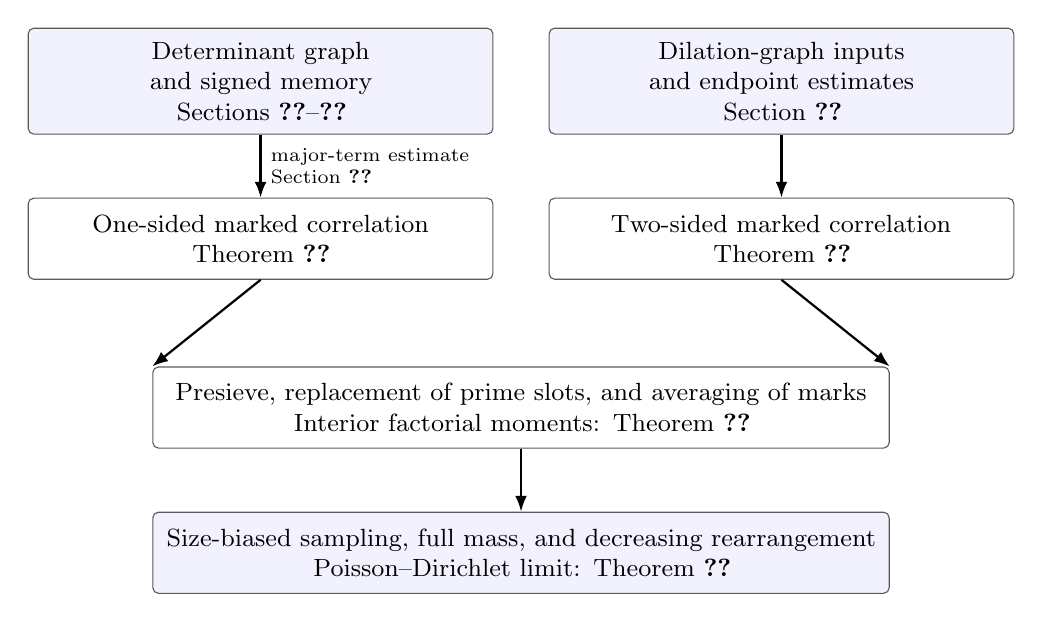
\begin{tikzpicture}[
  box/.style={draw=black!65,rounded corners=2pt,align=center,
    text width=5.55cm,minimum height=1.03cm,inner sep=5pt,font=\small},
  arr/.style={-{Latex[length=2mm]},thick},
  node distance=8mm and 7mm]
\node[box,fill=blue!5] (det)
  {Determinant graph and signed memory\\
   Sections~\ref{sec:determinant}--\ref{mem:section}};
\node[box,fill=blue!5,right=of det] (dil)
  {Dilation-graph inputs and endpoint estimates\\
   Section~\ref{sec:correlations}};
\node[box,below=of det] (one)
  {One-sided marked correlation\\Theorem~\ref{thm:type-II}};
\node[box,below=of dil] (two)
  {Two-sided marked correlation\\Theorem~\ref{thm:two-sided}};
\node[box,below=11mm of $(one.south)!.5!(two.south)$,
      text width=9cm] (interior)
  {Presieve, replacement of prime slots, and averaging of marks\\
   Interior factorial moments: Theorem~\ref{thm:interior}};
\node[box,below=of interior,text width=9cm,fill=blue!5] (pd)
  {Size-biased sampling, full mass, and decreasing rearrangement\\
   Poisson--Dirichlet limit: Theorem~\ref{thm:main}};
\draw[arr] (det) -- node[right,font=\scriptsize,align=left]
  {major-term estimate\\Section~\ref{sec:major-arcs}} (one);
\draw[arr] (dil) -- (two);
\draw[arr] (one.south) -- (interior.north west);
\draw[arr] (two.south) -- (interior.north east);
\draw[arr] (interior) -- (pd);
\end{tikzpicture}
\caption{The proof has two analytic inputs. The one-sided estimate
replaces prime slots in composite terms by rough slots. Successful
marking brings the resulting centered statistic under the two-sided
estimate. Averaging the fixed marks then gives interior moments;
the probability argument recovers the full law.
Appendix~\ref{lp:section} supplies the long-prime and
logarithmic-phase estimates used in the analytic branches.}
\label{fig:proof-map}
\end{figure}


\section{Conventions and analytic inputs}\label{sec:inputs}

Throughout the proof $x$ is a real parameter tending to infinity, and
\[
 L=\log x,\qquad W=\exp(L^{0.24}),\qquad
 V(W)=\prod_{p\le W}\left(1-\frac1p\right),\qquad
 \e(t)=\exp(2\pi i t).
\]
A positive integer is \emph{rough} if none of its prime factors is at
most $W$; we set $P^-(1)=\infty$.  Prime variables in explicitly
indicated prime sums range only over primes.  The functions $\tau(n)$
and $\tau_j(n)$ count divisors and ordered factorizations into $j$
positive integers, respectively.  Dirichlet characters are zero on
nonunits.  We use $n\asymp H$ for a fixed bounded enlargement of
$[H,2H]$.

Every unspecified exponent of $L$ is fixed before $x$ tends to
infinity.  Constants may depend on previously fixed data.  Whenever
an exponent must be independent of a marking parameter, this is
stated explicitly.  The number of determinant pads in
Sections~\ref{sec:determinant}--\ref{sec:major-arcs} grows slowly
with $L$; the padding parameter in Section~\ref{sec:correlations}
is instead a sufficiently large fixed integer.  These are separate
constructions.

We use the dilation-graph and ideal-kernel theorems of the companion
\emph{Weighted dilation graphs, smooth shifted primes and totient
fibers}~\cite{SmoothShifted}, denoted S. Its complete text accompanies
this article. Section~\ref{sec:correlations} states the exact operator
contracts and verifies their endpoint hypotheses. The long-prime and
logarithmic-phase estimates stated below are proved in
Appendix~\ref{lp:section}. Our presieving cutoff is always the $W$
defined above; it is not S's cutoff $\exp(\sqrt{\log x})$.

\subsection{Prime estimates and mean squares}

\begin{lemma}[Prime estimates]\label{lem:prime-estimates}
The prime number theorem holds with an error smaller than every
fixed negative power of the logarithm.  In particular, as $y\to\infty$,
\[
 \sum_{p\le y}\frac1p=\log\log y+c_M+o(1),
 \qquad
 \prod_{p\le y}\left(1-\frac1p\right)
       \sim\frac{e^{-\gamma_E}}{\log y},
\]
where $c_M$ and $\gamma_E$ are constants.  For fixed $A,C>0$,
uniformly for $r\le(\log y)^C$ and $(a,r)=1$,
\[
 \#\{p\le y:p\equiv a\pmod r\}
 =\frac{\Li(y)}{\varphi(r)}
     +O_{A,C}\!\left(\frac{y}{(\log y)^A}\right).
\]
The constants need not be effective.
\end{lemma}

These classical estimates follow from the quantitative prime number
theorem, Siegel--Walfisz, and Mertens' theorems; see
\cite[Corollary~39 and Exercises~40, 64]{TaoSW} and
\cite[Theorems~15, 26]{TaoMertens}. The harmonic asymptotic also follows
by partial summation of the prime number theorem. Thus, for every fixed $a>0$,
\begin{equation}\label{eq:band-mass}
 \sum_{\exp(L^a)\le p\le\exp(2L^a)}\frac1p
       =\log 2+o(1).
\end{equation}
We use prime asymptotics only on fixed positive-power ranges or on
intervals for which taking differences of the stated estimates gives
the required absolute error.

For the classical, stronger coefficient-independent mean-value
theorem, see \cite[Theorem~2 and Corollary~3]{MontgomeryVaughan1974}.
We prove the weaker bounds needed here directly.

\begin{lemma}[Divisor moments and Dirichlet mean squares]
\label{lem:moment-bounds}
For every fixed nonnegative integer $k$ there is $C_k$ such that
\[
 \sum_{n\le Y}\tau(n)^k\ll_k Y(\log(2Y))^{C_k},\qquad
 \sum_{n\le Y}\frac{\tau(n)^k}{n}
       \ll_k(\log(2Y))^{C_k}.
\]
Let $P(t)=\sum_{n\le Y}c_n n^{it}$.  On every real interval $I$
of length $T\ge0$,
\begin{align}
 \int_I|P(t)|^2\dd t
 &\ll (T+Y\log(2Y))\sum_n|c_n|^2,\label{eq:dirichlet-mean}\\
 \sum_{t\in\mathcal T}|P(t)|^2
 &\ll (T+1+Y\log(2Y))(\log(2Y))^2
                  \sum_n|c_n|^2,\label{eq:dirichlet-spaced}
\end{align}
whenever $\mathcal T\subset I$ has mutual spacing at least one.
The constants in these two inequalities are absolute and do not
depend on how the coefficients were formed.
\end{lemma}

\begin{proof}
Unique factorization and positivity bound the harmonic divisor sum by
\[
 \prod_{p\le Y}\sum_{a\ge0}\frac{(a+1)^k}{p^a}
 =\prod_{p\le Y}\left(1+\frac{2^k}{p}+O_k(p^{-2})\right)
 \ll_k (\log(2Y))^{C_k}.
\]
Multiplication by $Y$ gives the counting bound. For the continuous
mean square, expand the square and integrate. The diagonal is
$T\sum_n|c_n|^2$. For $m\ne n$, the integral has absolute value at
most $2/|\log(n/m)|\ll Y/|n-m|$. The inequality
$2|c_nc_m|\le |c_n|^2+|c_m|^2$ and the harmonic sum over $|n-m|$
give \eqref{eq:dirichlet-mean}. On the unit interval centered at each
point of $\mathcal T$, the one-dimensional Sobolev inequality bounds
$|P(t)|^2$ by a constant times the integral of $|P|^2+|P'|^2$.
These intervals have bounded overlap and lie in an interval of length
$T+1$. Apply the continuous estimate to $P$ and $P'$, whose
coefficients are $i(\log n)c_n$, to obtain
\eqref{eq:dirichlet-spaced}.
\end{proof}

The coefficient-independent formulation in
\eqref{eq:dirichlet-mean}--\eqref{eq:dirichlet-spaced} is important:
later a small-prime polynomial is raised to a growing power, whose
coefficient norm is bounded separately by a factorial estimate.
Fixed divisor moments alone are not applied at that growing order.

\subsection{Prime polynomials and logarithmic phases}

\begin{lemma}[Long prime polynomial]\label{lem:long-prime}
Fix $0<\tau<\eta<1$ and $C,A>0$.  There is
$B_0=B_0(\tau,\eta,C,A)$ such that, uniformly for
\[
 \frac{x^\tau}{2}\le N\le x^\eta,\qquad
 q\le L^C,\qquad L^{B_0}\le |t|\le x^2,
\]
every Dirichlet character $\chi$ modulo $q$ and every interval
$I\subset[N,2N]$ satisfy
\begin{equation}\label{eq:long-prime}
 \left|\sum_{p\in I}\chi(p)p^{-1+it}\right|
       \ll_{\tau,\eta,C,A}L^{-A}.
\end{equation}
\end{lemma}

The complete proof is Lemma~\ref{lp:prime-polynomial} in
Appendix~\ref{lp:section}, with exactly the displayed ranges. Partial
summation converts the reciprocal weight in \eqref{eq:long-prime}
to normalization by $N$ on a dyadic interval.

\begin{lemma}[Logarithmic phases on progressions]\label{lem:log-phase}
Fix $C>0$.  There is an absolute constant $C_3>0$ such that, for
sufficiently large $x$ in terms of $C$, the following holds uniformly:
\[
 \exp\!\left(\frac{L}{(\log L)^2}\right)\le N\le2x^5,
 \quad q\le L^C,
 \quad
 \exp\!\left(\frac{L}{2(\log L)^2}\right)\le |t|\le4x^3.
\]
For every residue $a\pmod q$ and every interval $I\subset[N,2N]$,
\begin{equation}\label{eq:log-phase}
 \left|\sum_{\substack{n\in I\\n\equiv a\pmod q}}n^{it}\right|
 \ll \frac Nq\exp\!\left(-\frac{L}{(\log L)^{C_3}}\right).
\end{equation}
\end{lemma}

The proof is Lemma~\ref{lp:log-phase} in Appendix~\ref{lp:section}.
The estimate applies to arbitrary residue
classes, not only units.  At lower frequencies we use the elementary
sum--integral comparison on a progression.  For $N\ge x^\delta$,
$q\le L^C$ and $1\le|t|\le\exp(L/(\log L)^2)$, it gives
\begin{equation}\label{eq:moderate-phase}
 \frac qN\left|\sum_{\substack{n\in I\\n\equiv a\pmod q}}n^{it}\right|
 \ll \frac1{|t|}+x^{-c_\delta},
\end{equation}
after decreasing $c_\delta>0$ if necessary.  Indeed the integral is
$O(N/(q|t|))$, and the endpoint/total-variation error is
$O(1+|t|)$.  The same estimate holds after partial summation against
a smooth factor with fixed logarithmic derivative costs, with those
costs included in the implied logarithmic power.

\subsection{Elementary rough counts}

\begin{lemma}[Rough integers in long intervals]\label{lem:rough-counts}
Fix $\delta>0$, $C>0$, $0<a<1$ and $A>0$.  Suppose
$x^\delta\le H\le x^C$ and $I\subset[H,2H]$ is an interval.
Then
\begin{equation}\label{eq:rough-count}
 \#\{n\in I:P^-(n)>W\}=V(W)|I|+O(HL^{-A}).
\end{equation}
If $d\le\exp(L^a)$ and every prime divisor of $d$ exceeds $W$,
then for every residue $b\pmod d$,
\begin{equation}\label{eq:rough-off-sieve-progression}
 \#\{n\in I:n\equiv b\pmod d,\ P^-(n)>W\}
 =\frac{V(W)|I|}{d}+O\!\left(\frac Hd L^{-A}\right).
\end{equation}
For every character $\chi$ modulo $q\le L^C$,
\begin{equation}\label{eq:rough-character}
 \sum_{\substack{n\in I\\P^-(n)>W}}\chi(n)
 =\1_{\chi\text{ principal}}V(W)|I|+O(HL^{-A}).
\end{equation}
All statements are uniform in the indicated intervals and residues.
\end{lemma}

\begin{proof}
Use consecutive even and odd Bonferroni truncations for the events
$p\mid n$, $p\le W$, at depths $h$ and $h+1$, with
$h\asymp C_A\log L$.  Their divisors are at most
\[
 W^{h+1}=\exp\bigl(O_A(L^{0.24}\log L)\bigr)=x^{o(1)}.
\]
The number of divisor terms and their total absolute integer
coefficient mass are also $x^{o(1)}$.  Counting each progression
by its length divided by the modulus costs at most one per term.
Writing $S_W=\sum_{p\le W}1/p=O(\log L)$, the difference of the
two model bounds is at most
\[
 \frac{S_W^{h+1}}{(h+1)!},
\]
which is smaller than any prescribed power of $L^{-1}$ on choosing
the fixed constant $C_A$ sufficiently large.  The full model product
is $V(W)$.

For \eqref{eq:rough-off-sieve-progression}, each sieve divisor is
coprime to $d$, so the Chinese remainder theorem gives main term
$|I|/(de)$ for the divisor $e$.  The same omitted-degree bound is
multiplied by $H/d$.  The total endpoint error remains $x^{o(1)}$,
which is smaller than $(H/d)L^{-A}$, since $d=x^{o(1)}$ and
$H\ge x^\delta$.  This proves both counting formulas.

For \eqref{eq:rough-character}, first count a fixed unit residue
class modulo $q$.  Primes dividing $q$ are automatically absent;
the model density in that progression is
\[
 \frac1q\prod_{\substack{p\le W\\p\nmid q}}
        \left(1-\frac1p\right)=\frac{V(W)}{\varphi(q)}.
\]
The endpoint and Bonferroni errors have arbitrary logarithmic
precision, uniformly for $q\le L^C$.  Sum with the character over
the unit residue classes, choosing the precision first to absorb
their number.  Character orthogonality gives the displayed answer.
\end{proof}

\subsection{A sieve for nonnegative weighted objects}

\begin{lemma}[Block sieve]\label{lem:block-sieve}
Consider finitely many objects with nonnegative weights and a bad
condition at each of some designated primes $p\le z$.  Suppose
that the total weight on which all conditions indexed by the primes
dividing a squarefree $d$ hold is
\[
 Xg(d)+r(d),
\]
including $d=1$, where $X\ge0$, $g$ is multiplicative, and fixed
$\eta_0>0,C_0$ satisfy
\[
 0\le g(p)\le1-\eta_0,
 \qquad \sum_{w<p\le w^2}g(p)\le C_0\quad(w>1).
\]
For every sufficiently large even integer $h$, the weight avoiding
all designated bad conditions is
\begin{equation}\label{eq:block-sieve}
 X\prod_{p\le z}(1-g(p))\bigl(1+O(e^{-h})\bigr)
 +O\!\left(\sum_{\substack{d\le z^{4h+2}\\d\text{ squarefree}}}
          |r(d)|\right).
\end{equation}
Products and sums use only designated primes.  Constants depend
only on the density bounds and are uniform in $h$.  For $h=2$,
an upper bound holds with a fixed constant times the main term
and the same remainder sum.
\end{lemma}

This is the block sieve of S~\cite[Lemma~2.9]{SmoothShifted}.
Its upper and lower polynomials have coefficients of absolute value
at most one, supported on squarefree $d\le z^{4h+2}$; the upper
polynomial is nonnegative.  We will supply all needed remainder
estimates for our particular weights.  No assertion detecting
primes from congruence information alone is included in this input.

\section{A determinant estimate with marks on one side}
\label{det:section}
\label{sec:determinant}

The first correlation estimate removes prime conditions from factors of
the unmarked endpoint.  Throughout this section and the next two sections,
put
\begin{equation}\label{det:parameters}
 L=\log x,\qquad W=\exp(L^{0.24}),\qquad
 V(W)=\prod_{p\leq W}(1-p^{-1}).
\end{equation}
An integer is \emph{rough} if it has no prime factor at most $W$.
Fix disjoint groups consisting of all the primes in the bands
\begin{equation}\label{det:bands}
 \mathcal P_i=\{p:\exp(L^{a_i})\leq p\leq\exp(2L^{a_i})\},
 \qquad 0.1<a_1<\cdots<a_K<0.2.
\end{equation}
Here $K$ and the $a_i$ are fixed before $x$ tends to infinity.  Write
\begin{equation}\label{det:marks}
 \begin{aligned}
 V_i&=\sum_{p\in\mathcal P_i}\frac1p,
 &\mu_i(p)&=\frac1{pV_i},\\
 \omega_i(h)&=\sum_{p\in\mathcal P_i}\1_{p\mid h},
 &\omega(h)&=\sum_{i=1}^K\omega_i(h).
 \end{aligned}
\end{equation}
Lemma~\ref{lem:prime-estimates} and partial summation give
$V_i=\log 2+o(1)$.  For a fixed $q\in(0,1)$, the marked weight is
\begin{equation}\label{det:weight}
 \mathcal W(h)=q^{\omega(h)-K}
       \prod_{i=1}^K\frac{\omega_i(h)}{V_i}.
\end{equation}
The weight is zero if some group supplies no divisor, and is bounded by
a constant depending only on $K,q$.  Indeed, $q^{j-1}j$ is bounded for
positive integers $j$.

\begin{theorem}[One-sided marked Type II estimate]\label{thm:type-II}
Fix $\delta,C,D_*>0$ and $q\in(0,1)$.  Suppose
$H_m,H_n\geq x^\delta$ and $X=H_mH_n\asymp x$.  Let $F$ satisfy
$|F(h)|\leq1$ and $F(ph)=F(h)$ for every prime in the groups
\eqref{det:bands}.  Let $\alpha_m$ be supported on an arbitrary
interval in $[H_m,2H_m]$, where it has the value
\[
 \alpha_m=m^{iv}\left(\1_{m\text{ prime}}
       -\frac{\1_{m\text{ rough}}}{V(W)\log m}\right),
 \qquad |v|\leq L^C.
\]
Let $\beta_n$ be supported on rough integers in $[H_n,2H_n]$, with
$|\beta_n|\leq L^C$.  If $K$ is sufficiently large in terms of
$\delta,C,D_*,q$, then
\begin{equation}\label{eq:type-II}
 \left|\sum_{m,n}\alpha_m\beta_n F(mn-1)\mathcal W(mn-1)\right|
       \ll X L^{-D_*}.
\end{equation}
The required lower bound on $K$ is independent of the particular
$a_i$.  The implicit constant and the threshold for $x$ may depend on
all the fixed parameters, including the $a_i$.
\end{theorem}

We first give the reduction and geometric construction.  The signed
moment estimate is proved in Proposition~\ref{prop:minor-moment};
Proposition~\ref{prop:major-term} estimates the resulting major term
and completes the proof of the theorem.  Exponents denoted $O_C(1)$
below can be chosen independently of $K$.  A factor depending on a
fixed $K$ is harmless, but a loss $L^{cK}$ would not be harmless at
the final choice of $K$; we keep this distinction explicit.

\subsection{Cauchy's inequality and the normalization of the square}

Expand the product of the $\omega_i$ by selecting one prime from
each group, and denote their product by $b_0$.  For $mn-1=b_0h$,
invariance gives $F(mn-1)=F(h)$.  Except when some selected prime
has square dividing $mn-1$, one also has
$\omega(h)=\omega(mn-1)-K$.  The replacement of the original
damping by $q^{\omega(h)}$ costs
\begin{equation}\label{det:squareful-error}
 O_A(XL^{-A})\qquad\text{for every fixed }A>0.
\end{equation}
To verify this, the sum over labels of either nonnegative weight is
$O_{K,q}(1)$: removing $K$ distinct prime factors can lower $\omega$
by at most $K$, so the new weight is at most the old one.
For fixed $m$ and a group prime $p$, the congruence
$mn\equiv1\pmod {p^2}$ either has no solution or specifies one
residue class of $n$.  Since $H_n\geq x^\delta\gg p^2$, its count
is $O(H_n/p^2)$.  Finally
$\sum_{i,p\in\mathcal P_i}p^{-2}\ll_K\exp(-L^{0.1})$.
The coefficient bounds absorb only a fixed power of $L$, proving
\eqref{det:squareful-error}.

Choose a real smooth dyadic partition with factors $\eta(b_0/Y)$,
where $\eta$ is supported in $[1,4]$ and has bounded derivatives.
There are $O_K(L)$ relevant $Y$, and
\begin{equation}\label{det:Y-range}
 cL^{0.1}\leq\log Y\leq C_KL^{0.2}.
\end{equation}
For a fixed factor of this partition the sum becomes
\[
 \sum_{h\ll X/Y}F(h)q^{\omega(h)}
 \sum_{\substack{mn-1=b_0h\\b_0=\prod_i p_i,\ p_i\in\mathcal P_i}}
       \left(\prod_iV_i^{-1}\right)
       \eta(b_0/Y)\alpha_m\beta_n.
\]
Cauchy's inequality bounds its square by $O(X/Y)$ times the
nonnegative expanded square
\begin{equation}\label{det:cauchy-square}
 \begin{split}
 \mathcal Q_Y={}&\left(\prod_iV_i^{-2}\right)
 \sum_{\substack{a,b,m,n,r,s\\mn-1=ah,\ rs-1=bh\text{ for some }h}}
 \eta(a/Y)\eta(b/Y)
 \alpha_m\overline{\alpha_r}\beta_n\overline{\beta_s}.
 \end{split}
\end{equation}
Both $a$ and $b$ select one prime per group.  In particular, proving
$\mathcal Q_Y\ll XYL^{-D_1}$ for arbitrarily large fixed $D_1$
is sufficient; the required $D_1$ depends on $C,D_*$ but not on $K$.

We may first discard pairs $a,b$ sharing a label.  The elementary
bound used here, uniform for $l\asymp Y$, is
\begin{equation}\label{det:progression-divisors}
 \sum_{h\ll X/Y}\tau(1+lh)^2\ll (X/Y)L^3.
\end{equation}
Indeed, $\tau(n)^2\leq\tau_4(n)$.  In an ordered four-factor
decomposition of an integer at most $O(X)$, deleting a largest
factor leaves a product $d\ll X^{3/4}$.  There are at most
$4\tau_3(d)$ choices for the three retained factors and their
positions.  If $d\mid1+lh$, then $(d,l)=1$, and $h$ lies in one
progression modulo $d$.  Consequently the left side of
\eqref{det:progression-divisors} is at most a constant times
\[
 \sum_{d\ll X^{3/4}}\tau_3(d)\left(\frac{X}{Yd}+1\right)
 \ll \frac XY L^3+X^{3/4}L^2\ll\frac XY L^3.
\]
These divisor estimates also follow from Lemma~\ref{lem:moment-bounds}.
For fixed $a,b$, Cauchy's inequality and
\eqref{det:progression-divisors} bound the absolute $h$-sum of the
two representation counts by $(X/Y)L^{O_C(1)}$.
The number of pairs sharing a prime is
\[
 \ll Y^2\sum_{i,p\in\mathcal P_i}p^{-2}
 \ll_K Y^2\exp(-L^{0.1});
\]
here the number of integers in $[Y,4Y]$ divisible by $p$ is
$O(Y/p)$.  Thus the discarded part is $O_A(XYL^{-A})$.

For the remaining pairs $(a,b)=1$.  Their two equations in
\eqref{det:cauchy-square} are equivalent to
\begin{equation}\label{det:equation}
 t=bmn-ars=b-a.
\end{equation}
In fact, the displayed equality gives $a\mid mn-1$ and
$b\mid rs-1$, and the quotients agree and are positive.

Fix a real compactly supported smooth $\psi$, equal to one on
$[-4,4]$.  For a fixed exponent $A_0>0$, let $\mathfrak M$ be the
union, on $\R/\Z$, of the arcs
\[
 \left|\theta-\frac hk\right|\leq\frac{2L^{A_0}}Y,
 \qquad 1\leq k\leq L^{A_0},\quad (h,k)=1.
\]
They are disjoint for large $x$.  The replacement for
\eqref{det:equation} is
\begin{equation}\label{eq:det-major}
 \mathcal H_{\mathfrak M}(t;a,b)
   =\psi(t/Y)\int_{\mathfrak M}
                  \e\bigl(\theta(t-b+a)\bigr)\,\dd\theta.
\end{equation}
In the ultimate major sum $a,b$ need not be disjoint.  The signed
error in this replacement is controlled by the lift constructed
next.

\subsection{Physical states, good positions, and endpoint vectors}

Use the growing parameters
\begin{equation}\label{det:moment-parameters}
 J=\lfloor L^{0.01}\rfloor,\quad M=J+1,\quad
 R=\lceil L^{0.5}/2\rceil,\quad N=2R.
\end{equation}
An auxiliary list has $J$ primes per group; its product is denoted
by $D$.  Partition all possible $D$ into ordinary dyads
$[d_0,2d_0)$.  There are $O_K(L)$ such dyads and
$\log(2d_0)\leq C_KL^{0.21}$.  Fix one and put
\begin{equation}\label{det:physical-box}
 H=d_0Y,\qquad U=HH_m,\qquad V=H_n,\qquad
 \Omega=[U,16U]\times[V,2V].
\end{equation}

A \emph{physical state} is a primitive integer vector
$P=(P_1,P_2)\in\Omega$ together with an ordered list
$\boldsymbol p_i=(p_{i,1},\ldots,p_{i,M})$ of distinct primes
from $\mathcal P_i$ for each $i$, all dividing $P_1$.
Let $\mathcal H$ be the Hilbert space on these states with measure
\begin{equation}\label{det:state-measure}
 \dd\sigma(P,\boldsymbol p)=\prod_{i=1}^KV_i^{-M}
 \quad\text{times counting measure}.
\end{equation}
Averaging independently over permutations of each list defines an
orthogonal projection $\mathcal S$ on $\mathcal H$.

We now specify the row operation before symmetrization.  Copy slots
$1,\ldots,J$ in every group from source to target; their product
is $D$.  The product of the source's last slots is $b$.  The
target's last slots are new labels with product $a$.  Each new
slot is summed with weight $V_i^{-1}$; target positions are summed
with counting measure.  The labels shared across the edge are
exactly the copied slots.  Thus all unshared labels are distinct
from one another and from every shared label, including across
the two endpoints.  This restriction will be called the
\emph{cross-edge ban}.  Require $D\in[d_0,2d_0)$ and
$t=\det(P,Q)/D\in\Z$, and use the multiplier
\begin{equation}\label{eq:det-kernel}
 \begin{split}
 \mathcal K(P,Q;D,a,b)={}&\frac{d_0}{D}
       \eta(b/Y)\eta(a/Y)\psi(t/Y)\\
 &\times\left\{\1_{t=b-a}
       -\int_{\mathfrak M}\e\bigl(\theta(t-b+a)\bigr)
                    \,\dd\theta\right\}\\
 &\times q^{(\omega(P_1)-KM)/2+(\omega(Q_1)-KM)/2}.
 \end{split}
\end{equation}
Let $\mathcal T$ be this row operation. All sums are finite.
The adjoint reverses the row rule and
conjugates its multiplier.  Indeed, the joint measure of the two
lists in an edge pairing is $\prod_iV_i^{-(M+1)}$ in either
direction: one factor $V_i^{-M}$ comes from
\eqref{det:state-measure}, and one $V_i^{-1}$ from the new slot.

After slot symmetrization, the copied products $D$ range over all choices
obtained by omitting one prime from each full list and lying in the chosen
pad dyad $[d_0,2d_0)$. Each of the $M^K$ omission tuples has weight
$M^{-K}$ under the source symmetrization.

We next restrict the positions at which this row operation is used.
The first restriction will keep the lattice determined by the shared
labels from becoming too thin. The second separates phases associated
with the omission choices; in the repeated-prime argument it will leave
at most one compatible omission tuple.

For a primitive $P$, complete it to an integral matrix of determinant
one, and let $r_P$ be the first coordinate of the second column
divided by $P_1$, considered modulo one.  Changing the completion
adds an integer, so $r_P$ is well defined.  A position with its
full unordered lists is \emph{good} if the following hold.
\begin{enumerate}[label=(\roman*)]
\item\label{det:good-first} For every $D\in[d_0,2d_0)$ obtained by
omitting one label per group, there is no integer
$1\leq l\leq Y^{0.2}$ such that
$\|lDr_P\|_{\R/\Z}\leq Y^{-0.7}$.
\item\label{det:good-second} Let $I$ be any nonempty subset of the
groups and $i_* =\max I$.  Draw one fresh prime in each group
outside $I$, independently according to $\mu_i$, and let $T_f$
be their product.  Except for a set of these draws of probability
at most $\exp(-\tfrac14L^{a_{i_*}})$, the points
$DZ T_f r_P$ corresponding to all distinct integers $DZ$ are
pairwise separated in circle distance by
$100\exp(-L^{a_{i_*}})$.  Here $D$ ranges over the omission
products just described, and $Z$ selects one prime from each
group in $I\setminus\{i_*\}$.
\end{enumerate}
Let $\mathcal G$ be the projection onto good states. The definition
is symmetric in the ordered slots, so $\mathcal G$ commutes with
$\mathcal S$. We use the restricted, symmetrized operator
\[
 \mathcal A=\mathcal G\mathcal S\mathcal T\mathcal S\mathcal G.
\]
The first test is used in the lattice construction leading to
\eqref{mem:lattice-shape}; the second is used to prove the unique
omission choice in the argument following \eqref{mem:anchor-congruence}.

\begin{lemma}\label{det:good-state}
For any fixed lists, the set of $r\in\R/\Z$ failing goodness has
Lebesgue measure at most $\exp(-cL^{0.1})$, for some $c>0$ and
all sufficiently large $x$.
\end{lemma}
\begin{proof}
There are at most $M^K$ omission products.  The union bound for
the first test is at most $2M^KY^{-0.5}$, which has the required
size by \eqref{det:Y-range}.  For the second test fix $I,T_f$.
The number of trial integers $DZ$ is
\[
 M^K\prod_{i\in I\setminus\{i_*\}}|\mathcal P_i|
          =\exp\bigl(o(L^{a_{i_*}})\bigr).
\]
For distinct $DZ,D'Z'$, the integer
$(DZ-D'Z')T_f$ is nonzero.  Multiplication by this integer
preserves uniform measure on the circle.  The measure on which
this pair violates the required separation is therefore at most
$200\exp(-L^{a_{i_*}})$.  Summing over pairs and then averaging
over $T_f$ gives $\exp(-L^{a_{i_*}}+o(L^{a_{i_*}}))$.
Markov's inequality at the threshold
$\exp(-\tfrac14L^{a_{i_*}})$ gives
$\exp(-\tfrac34L^{a_{i_*}}+o(L^{a_{i_*}}))$ for the exceptional
set of $r$.  There are only $2^K-1$ possible $I$.
\end{proof}

We record precisely the vectors that recover the Cauchy square.
At an endpoint require the complete part of $P_1$ supported on
the group primes to be squarefree, with exactly $M$ primes from
each group.  Denote that part by $G(P_1)$.  Put
\begin{equation}\label{det:endpoints}
 \overline{f(P)}=\alpha_{P_1/G(P_1)}\overline{\beta_{P_2}},
 \qquad
 g(P)=\overline{\alpha_{P_1/G(P_1)}}\beta_{P_2},
\end{equation}
and set these vectors to zero when the stated conditions or the
coefficient supports fail.  The vectors are constant on lists.
In an edge contributing to their pairing, the coordinates are
\begin{equation}\label{det:lift}
 P=(Dbm,s),\qquad Q=(Dar,n),\qquad
 \det(P,Q)/D=bmn-ars.
\end{equation}
No new restriction is imposed on the original coefficients:
every $m,r,n,s$ with nonzero coefficient is rough, and every
group prime is below $W$.  The damping in
\eqref{eq:det-kernel} equals one at these endpoints.

Their norms have the uniform bounds
\begin{equation}\label{det:endpoint-norms}
 \|f\|,\|g\|\ll(UV)^{1/2}L^{O_C(1)},\qquad
 \sup|f|+\sup|g|\ll L^{O_C(1)}.
\end{equation}
For example, at a fixed ordered list with product $G$, the number
of possible positions is $O(UV/G)$, since $G=x^{o(1)}\ll U$.
Summing its reciprocal product with the state normalization gives
\[
 \prod_i V_i^{-M}
 \sum_{\substack{p_{i,1},\ldots,p_{i,M}\in\mathcal P_i\\
                  \text{distinct in each group}}}
             \prod_{i,j}\frac1{p_{i,j}}\leq1.
\]
This proves \eqref{det:endpoint-norms} without a logarithmic
exponent depending on $K$ or $J$.

Conversely, positions in \eqref{det:lift} on the support of
\eqref{eq:det-kernel} are automatically primitive.  A prime
dividing both $Dbm$ and $s$ cannot divide $Db$, by roughness.
It would therefore divide $m,s$ and be larger than $W$.  It then
divides $t=bmn-ars$.  The cutoff gives $|t|\ll Y<W$, so $t=0$.
But $bmn=ars$ is impossible: any prime in $b$ divides none of
$a,r,s$.  The same proof applies to $Q$.  The ranges in
\eqref{det:lift} lie in \eqref{det:physical-box} because
$D\in[d_0,2d_0)$ and $a,b\in[Y,4Y]$.

\subsection{From the moment to endpoint pairings}

For a primitive $P\in\Omega$, let $\mathbf u_P$ be one on every
list at $P$ and zero at other positions.  These vectors are not
normalized.  The estimate proved in
Proposition~\ref{prop:minor-moment} is, for any prescribed $E_0>0$,
\begin{equation}\label{eq:det-moment}
 \frac1{UV}\sum_{P\in\Omega\text{ primitive}}
       \langle\mathbf u_P,(\mathcal A\mathcal A^*)^R
                     \mathbf u_P\rangle
             \leq L^{-E_0N}.
\end{equation}
First $A_0$ and then $K$ are chosen sufficiently large; thresholds
in absolute errors may subsequently depend on the fixed group
exponents.  We prove here the consequence
\begin{equation}\label{eq:det-pairing}
 |\langle f,\mathcal A g\rangle|
             \ll UVL^{-E_0+O_C(1)}.
\end{equation}

Partition positions into half-open intervals of the slope $P_2/P_1$
of length $H/U^2$.  A nonzero edge has
$|\det(P,Q)|\ll H$, so only a bounded number of neighboring
intervals can interact.  Each interval contains $O(H)$ primitive
positions.  To see this, choose a primitive pivot in it.  Its
determinant with any other position in the interval is an integer
of size $O(H)$.  With that determinant fixed, all integer
solutions differ by integral multiples of the pivot; the first
coordinate ranges over $[U,16U]$, permitting $O(1)$ multiples.

Let $f_j$ be $f$ restricted to one interval, and $g_j$ the
restriction of $g$ to its interacting neighbors.  Set
$B_0=\mathcal A\mathcal A^*$ and
\[
 d_j=\sum_{P\text{ in interval }j}
              \langle\mathbf u_P,B_0^R\mathbf u_P\rangle.
\]
The matrix $C^{(j)}_{PQ}=\langle\mathbf u_P,B_0^R\mathbf u_Q\rangle$
is positive semidefinite on the ordinary coefficient space.
Its largest eigenvalue is at most its trace $d_j$, irrespective
of the norms or orthogonality of the testing vectors.  Since
$f_j=\sum_P f(P)\mathbf u_P$, this gives
\begin{equation}\label{det:compression}
 \langle f_j,B_0^Rf_j\rangle
      \leq d_j\sum_P|f(P)|^2
      \ll H\sup|f|^2d_j.
\end{equation}
Spectral H\"older for the positive operator $B_0$, followed by
Cauchy's inequality, now gives
\[
 |\langle f_j,\mathcal A g_j\rangle|
 \leq \|g_j\|\,\|f_j\|^{1-1/R}
             \bigl(CH\sup|f|^2d_j\bigr)^{1/(2R)}.
\]
H\"older's inequality in $j$, with exponents
$2,2R/(R-1),2R$, and bounded overlap of the $g_j$ imply
\[
 |\langle f,\mathcal A g\rangle|
 \ll\|g\|\,\|f\|^{1-1/R}
       (CH\sup|f|^2)^{1/(2R)}
       \left(\sum_jd_j\right)^{1/(2R)}.
\]
By \eqref{det:Y-range} and \eqref{det:physical-box},
$\log H=O_K(L^{0.21})$, so $H^{1/N}=O(1)$.
Equations~\eqref{eq:det-moment} and
\eqref{det:endpoint-norms} prove \eqref{eq:det-pairing}.
This argument uses the unnormalized trace in
\eqref{eq:det-moment}; no normalization by the number of lists
has been introduced.

\subsection{Uniform residues at a primitive root}

The root average in \eqref{eq:det-moment} will be replaced by
independent projective residue lines.  We give an elementary
count that works even when the two coordinate scales are
comparable.  For a primitive $(u,v)$ in $\Omega$ there is a
unique completion
\begin{equation}\label{det:root-matrix}
 g=\begin{pmatrix}u&c\\v&d\end{pmatrix},\qquad
 ud-vc=1,\qquad 0\leq c<u.
 \quad\text{Put }r=c/u.
\end{equation}

\begin{lemma}[Root residues]\label{lem:root-residue}
There is $c_\delta>0$ such that the following holds.  Let $S$ be
squarefree with $S\leq\exp(C_KL^{0.98})$, and prescribe
$g_0\in\mathrm{SL}_2(\Z/S\Z)$.  If $I_1,I_2,I_3$ are intervals
in $[1,16],[1,2],[0,1]$, respectively, the number of primitive
roots satisfying
\[
 u/U\in I_1,\qquad v/V\in I_2,\qquad r\in I_3,
 \qquad g\equiv g_0\pmod S
\]
is
\begin{equation}\label{det:root-residue-count}
 \frac{UV\,|I_1||I_2||I_3|}
      {\zeta(2)|\mathrm{SL}_2(\Z/S\Z)|}
             +O(UVx^{-c_\delta}).
\end{equation}
The error is uniform in the intervals and in $g_0$.
\end{lemma}

\begin{proof}
We first prove the elementary exponential-sum estimate needed for
the count.  For $m\geq1$ put
\[
 K_m(h,k)=\sum_{y\in(\Z/m\Z)^\times}
                   \e\left(\frac{hy+ky^{-1}}m\right).
\]
Orthogonality shows that
$\sum_{h,k\bmod m}|K_m(h,k)|^4=m^2T_m$, where $T_m$ counts
unit quadruples $(y_1,y_2,z_1,z_2)$ with equal sums and equal
inverse sums.  The first relation determines
$z_2=y_1+y_2-z_1$.  After multiplying the inverse-sum relation
by the product of the four units, one obtains
\[
 m\mid(y_1+y_2)(z_1-y_1)(z_1-y_2).
\]
The map from the three free residues to these three linear forms
has determinant of absolute value two, and its kernel modulo
$m$ has size at most two.  Distribute, prime by prime, the
valuation of $m$ among the three factors.  There are
$\tau_3(m)$ distributions $d_1d_2d_3=m$; for each, the number
of triples of forms with the prescribed divisibilities is
$m^3/(d_1d_2d_3)=m^2$.  Consequently
$T_m\leq2m^2\tau_3(m)$.

The value of $K_m(h,k)$ is constant on the unit-scaling orbit
$(h,k)\mapsto(hs,ks^{-1})$.  If $g=(h,k,m)$, its stabilizer
consists of the units $s\equiv1\pmod{m/g}$, so the orbit has
$\varphi(m/g)\geq(m/g)m^{-o(1)}$ elements.  Dividing the fourth
moment bound by this orbit size gives
\begin{equation}\label{det:weak-kloosterman}
 |K_m(h,k)|\ll m^{3/4+o(1)}(h,k,m)^{1/4}.
\end{equation}
Only the elementary bounds $\tau_3(m)=m^{o(1)}$ and
$\varphi(m)\geq m^{1-o(1)}$ enter here; both follow by separating
the finitely many small primes from the remaining prime factors.

Suppose first $U\leq V$.  Write the entries of the prescribed
matrix as $u_0,c_0,v_0,d_0'$; the prime on $d_0'$ distinguishes
it from the pad scale.  Fix $u\equiv u_0\pmod S$.  Modulo
$m_0=uS$, the required pairs $(c,v)$ satisfy
\begin{equation}\label{det:fixed-u-congruences}
 c\equiv c_0\pmod S,\quad v\equiv v_0\pmod S,
 \quad cv\equiv ud_0'-1\pmod{uS}.
\end{equation}
There are exactly
\begin{equation}\label{det:fixed-u-mass}
 M(u)=u\prod_{\substack{p\mid u\\p\nmid S}}(1-p^{-1})
\end{equation}
such pairs.  Indeed, the admissible $c$ must be coprime to $u$.
At primes common to $u,S$ this is forced by
$u_0d_0'-c_0v_0=1$ modulo $S$; at other primes the indicated
Euler factors count the admissible $c$ in its progression.
For any such $c$, writing $v=v_0+Sj$ reduces the last congruence
to a linear congruence modulo $u$ with invertible coefficient
$c$, and hence determines exactly one $j\pmod u$.

These $M(u)$ pairs have discrepancy
\begin{equation}\label{det:modular-discrepancy}
 O(u^{0.99}S^2)
\end{equation}
for rectangles in the torus $(c/(uS),v/(uS))$.  Here are details
of the uniformity in $S$.  Put
$S_1=\prod_{p\mid(S,u)}p$ and $S_2=S/S_1$.  The Chinese
remainder theorem fixes $(c,v)$ modulo $S_2$ and leaves an
inverse graph modulo $m_1=uS_1$.  Write $a'=ud_0'-1$ and
$\gamma=S_2^{-1}\pmod {m_1}$; both are units modulo $m_1$.
On the inverse graph $cv=a'$ the condition $c\equiv c_0\pmod
{S_1}$ already forces $v\equiv v_0\pmod {S_1}$, since $c_0$
is a unit there.  Additive orthogonality thus gives the Fourier
sum, up to a constant of absolute value one, as
\begin{equation}\label{det:CRT-Fourier}
 \frac1{S_1}\sum_{j\bmod S_1}\e(-jc_0/S_1)
          K_{m_1}(\gamma h+ju,\gamma k a').
\end{equation}
For $0<\max(|h|,|k|)\leq u^{0.02}$,
\[
 (\gamma h+ju,\gamma ka',m_1)
      \leq S_1(h,k,u)\leq S_1u^{0.02}.
\]
Using the exponent $3/4+1/200$ in
\eqref{det:weak-kloosterman}, each nonzero sum
\eqref{det:CRT-Fourier} is therefore $O(u^{0.76}S^2)$.

For completeness, sandwich each interval indicator between
smooth upper and lower functions obtained by enlarging or
contracting the interval by $2u^{-0.01}$ and convolving with
a probability bump of width $u^{-0.01}$.  Their zeroth
coefficients differ from the interval length by $O(u^{-0.01})$.
Their Fourier coefficients are bounded.  There are $O(u^{0.04})$
retained frequency pairs, whose total cost is $O(u^{0.80}S^2)$.
For explicit control of the tail, if $\Delta=u^{-0.01}$ and
$T_1=u^{0.02}$, ten integrations by parts give a double
Fourier tail outside $\max(|h|,|k|)\leq T_1$ bounded by
$O(\Delta^{-11}T_1^{-9})=O(u^{-0.07})$.  The trivial bound
$M(u)\leq u$ makes its contribution $O(u^{0.93})$.
The error from the zeroth coefficient is $O(u^{0.99})$.
This proves \eqref{det:modular-discrepancy}.

The $c$ interval has length $u|I_3|$, and the $v$ interval has
length $V|I_2|$.  If the latter passes through several periods
of length $uS$, apply the rectangle count to each; the number
of pieces is $O(V/u+1)$.  Equations
\eqref{det:fixed-u-mass}--\eqref{det:modular-discrepancy} give
the fixed-$u$ main term
\[
 \frac{V|I_2||I_3|}{S^2}
           \prod_{\substack{p\mid u\\p\nmid S}}(1-p^{-1})
\]
and error $O((V/u+1)u^{0.99}S^2)$.
For $u\asymp U$ the sum of these errors is
$O(UV U^{-0.01}S^2)$.

It remains to average the Euler factor in the progression of
$u$.  Expanding it as
$\sum_{l\mid u,(l,S)=1}\mu(l)/l$ gives
\[
 \sum_{\substack{u/U\in I_1\\u\equiv u_0\ (S)}}
 \prod_{\substack{p\mid u\\p\nmid S}}(1-p^{-1})
 =\frac{U|I_1|}{S}
       \sum_{(l,S)=1}\frac{\mu(l)}{l^2}+O(\log(2U)).
\]
The tail beyond $16U$ contributes $O(1/S)$ and is covered by
the error.  The series equals
$\zeta(2)^{-1}\prod_{p\mid S}(1-p^{-2})^{-1}$.
Counting first columns and their completions over each field
shows
\begin{equation}\label{det:SL-order}
 |\mathrm{SL}_2(\Z/S\Z)|
       =S^3\prod_{p\mid S}(1-p^{-2}).
\end{equation}
This proves the stated main term.  Since $U\geq x^\delta$ and
$S^2=x^{o(1)}$, all the errors admit a saving $x^{-c_\delta}$;
for example, $c_\delta=\delta/1000$ is sufficient.

If $V<U$, fix $v$ instead and apply the same argument to the
congruence $ud\equiv1+vc_0\pmod{vS}$, with the roles of the
coordinates reversed and determinant sign reversed.  Use
$d/v$ as the third coordinate.  For $u,v>1$ both $c/u$ and
$d/v$ belong to $[0,1)$, and
\[
 \frac dv-\frac cu=\frac1{uv}.
\]
Enlarging and contracting the prescribed interval by
$O((UV)^{-1})$ changes its main mass by $O(1)$ and its count
by the already available discrepancy.  The same formula follows.
\end{proof}

\subsection{Independent residue lines and the archimedean error budget}

Expand \eqref{eq:det-moment} as a path with $N$ edges, returning
to its initial position but with no return condition on the
lists.  In the basis \eqref{det:root-matrix}, each position is
$gz$ with primitive $z\in\Z^2$, and the initial and final
vectors are $e_1=(1,0)$.  Put $\tau(z)=z_1+rz_2$.  The cutoff
and the physical box imply
\begin{equation}\label{det:tube}
 |z_2|\ll NH,\qquad |z_1|\ll NH,\qquad \tau(z)\asymp1.
\end{equation}
Indeed, one edge changes slope by $O(H/U^2)$; summing at most
$N$ changes gives $z_2=\det((u,v),gz)=O(NH)$.
Also $(gz)_1=u\tau(z)\asymp U$, which proves the remaining
claims.  For a group prime $p$, the condition $p\mid(gz)_1$
means that the projective line $[z]_p$ equals the kernel line
of the first row of $g$ modulo $p$.

\begin{lemma}[Replacement of the root average]\label{det:root-replacement}
In the normalized path expansion of \eqref{eq:det-moment}, one
may replace the root average by
\[
 \frac1{\zeta(2)}\int_{[1,16]\times[1,2]\times[0,1]}
                  \dd(u/U)\,\dd(v/V)\,\dd r
\]
and by independent uniformly distributed lines in
$\mathbb P^1(\mathbb F_p)$ for all the group primes.  The real
matrix at an archimedean root is
\[
 g(u,v,r)=\begin{pmatrix}u&ur\\v&vr+1/u\end{pmatrix}.
\]
All box and good-state conditions are retained.  The total error
is $O_A(L^{-AN})$ for every fixed $A>0$.  The same assertion,
with polynomial logarithmic coefficient bounds, holds for one
edge and for failure of either endpoint's goodness.
\end{lemma}

\begin{proof}
We specify both the combinatorial and the archimedean budgets.
There are $\exp(O_K(L^{0.73}))$ choices for paths $z$ satisfying
the size bounds in \eqref{det:tube}, labels of all visits, and
slot permutations.  For example, the logarithm of the number
of position paths is $O(N\log(NH))=O_K(L^{0.71})$;
the label choices have logarithm at most
$O_K(NML^{0.2})=O_K(L^{0.71})$; and the permutations cost
$O_K(NM\log M)$.  These also bound the total absolute
coefficients after dropping congruences and bounded damping.
The product of the primes active anywhere on a path has
logarithm $O_K(L^{0.72})$.

Keep the exact factors of the primes active at some visit.
At the other primes the joint damping can be written $1-X_p$,
where $0\leq X_p\leq1$.  Here the damping exponent at an
endpoint is $q_j=\sqrt q$ and at an interior visit is $q_j=q$.
In the independent-line model,
\[
 \sum_p\E X_p
 \leq\sum_p\sum_{j=0}^N\frac{1-q_j}{p+1}
 \ll_K N+1.
\]
Upper and lower Bonferroni polynomials of consecutive degrees
near $T=\lceil L^{0.76}\rceil$ sandwich
$\prod_p(1-X_p)$ pointwise.  Their expected difference is at
most
\[
 \frac{(C_K(N+1))^T}{T!}
       =\exp\bigl(-\Omega(L^{0.76}\log L)\bigr).
\]
The product inequality is ordinary inclusion--exclusion, applied
to numbers in $[0,1]$; it requires no independence for the
pointwise sandwich.  Independence between different residue
lines is used only to estimate its gap.  This gap absorbs the
$\exp(O_K(L^{0.73}))$ path and coefficient budget.

Each monomial in the truncated expressions requires residues at
the active primes and at most $T$ further primes.  Its squarefree
modulus satisfies
$\log S=O_K(L^{0.96})$, and hence lies in the range of
Lemma~\ref{lem:root-residue}.  The total number of monomials,
prime choices, and residue matrices is $\exp(o(L))$.
The uniform distribution on $\mathrm{SL}_2(\Z/S\Z)$ factors
over the primes by the Chinese remainder theorem.  At each
prime its first row is uniform among nonzero rows, and its
kernel is uniform among the $p+1$ projective lines.  This is
exactly the asserted independent model, with primitive-root
density $1/\zeta(2)$.

We next make the archimedean conditions compatible with interval
counts.  Choose an integral complement $w$ to each primitive
$z$, with $\det(z,w)=1$ and $|w|\ll1+|z|$.  The ratio for the
position $gz$ is
\begin{equation}\label{det:transported-ratio}
 r_{gz}=\frac{\tau(w)}{\tau(z)}\pmod1.
\end{equation}
On $\tau(z)\asymp1$ its derivative in $r$ is
$1/\tau(z)^2$.  The good tests are therefore constant except
at $\exp(o(L))$ values of $r$: enumerate every product and
fresh draw in the tests, every pair of distinct integers $DZ$,
and the integer translates in each circle inequality.
All their numbers and sizes are $\exp(o(L))$.
The exceptional-probability condition in the second good test
is also constant between these endpoints, because it is a
finite weighted sum of such indicators.

The physical coordinates are
\begin{equation}\label{det:transported-position}
 (gz)_1=u\tau(z),\qquad
 (gz)_2=v\tau(z)+z_2/u.
\end{equation}
The normalized box faces consequently have derivatives bounded
by $\exp(o(L))$.  Near a first-coordinate face the derivative
in $u/U$ is bounded below, and near a second-coordinate face
the derivative in $v/V$ is bounded below, because
$\tau(z)\asymp1$.  One may first exclude $\tau(z)$ near zero,
which is incompatible with the first-coordinate box condition.
Thus the union of cubes meeting any face or good-test boundary
has volume at most $x^{-\epsilon_\delta+o(1)}$ on a grid of
side $x^{-\epsilon_\delta}$ in $(u/U,v/V,r)$.

Choose the grid exponent only after the saving in
Lemma~\ref{lem:root-residue}; concretely take
$\epsilon_\delta=c_\delta/8$.  The grid has
$O(x^{3\epsilon_\delta})$ cubes, not a subpower number.
Summing all root-count errors, including the
$\exp(o(L))$ discrete choices, costs at most
\begin{equation}\label{det:grid-discrepancy}
 UVx^{-c_\delta+3\epsilon_\delta+o(1)}
       =UVx^{-5c_\delta/8+o(1)}.
\end{equation}
The main mass of boundary cubes is at most
\begin{equation}\label{det:grid-boundary}
 UVx^{-\epsilon_\delta+o(1)}
       =UVx^{-c_\delta/8+o(1)}.
\end{equation}
Their discrepancy is already included in
\eqref{det:grid-discrepancy}.  On each remaining cube all
archimedean indicator conditions are fixed.  The edge factors
in \eqref{eq:det-kernel} depend, after fixing labels, on
$\det(z,z')/D$ and hence do not vary with the root; the
finite residue factors have already been handled.
This proves the replacement with a fixed-power error after
normalization.  Such an error is $O_A(L^{-AN})$, since
$N\asymp L^{0.5}$.  The one-edge versions have smaller
enumeration budgets and use the same proof.
\end{proof}

It remains to bound the signed independent-line path expansion.
The next section keeps the precise correlations caused by a
prime that leaves an active list and later returns, proves
\eqref{eq:det-moment}, and then removes the good-state
projections and the auxiliary pads.  This yields the
replacement of \eqref{det:cauchy-square} by
\eqref{eq:det-major} with error $O_A(XYL^{-A})$.

\section{Signed memory and the determinant moment}
\label{mem:section}

We retain the notation, physical state space, good-state tests, and
operator $\mathcal A$ of the preceding section. In particular, the number
$J=\lfloor L^{.01}\rfloor$ of pads per group grows with $x$,
$M=J+1$, and $N=2R\asymp L^{.5}$. All constants depending on the fixed
number $K$ of groups are allowed to affect the threshold for $x$.
We will explicitly distinguish those constants from powers of $L$.

\begin{proposition}[The minor-arc moment]\label{prop:minor-moment}
For every fixed $E_0>0$, one can choose $A_0$ sufficiently large and then
$K$ sufficiently large, in terms of $E_0,q$ and the fixed parameters of
Theorem~\ref{thm:type-II}, so that the operator with the good-state
projections satisfies
\begin{equation}\label{mem:moment-bound}
 \frac{1}{UV}\sum_{\substack{P\in\Omega\\P\ \mathrm{primitive}}}
 \inner{\mathbf u_P}{(\mathcal A\mathcal A^*)^R\mathbf u_P}
 \le L^{-E_0N}.
\end{equation}
The choices of $A_0,K$ do not depend on the particular fixed band
exponents $a_1<\cdots<a_K$; the threshold for $x$ may depend on them.
Consequently, for any prescribed fixed $A>0$, the determinant indicator
in the expanded square of the preceding section can be replaced by
\eqref{eq:det-major}, with error $O_A(XY L^{-A})$. In the resulting
major term the disjointness restriction on the two unshared products
$a,b$ can be omitted. Equivalently, with the notation of
\eqref{det:cauchy-square} and \eqref{maj:sum},
\begin{equation}\label{mem:replacement-interface}
 \abs{\mathcal Q_Y-\mathcal Q_Y^{\mathrm{maj}}}
      \ll_A XY L^{-A}.
\end{equation}
The precision needed in the pairing estimate
\eqref{eq:det-pairing} for this consequence is independent of $K$.
\end{proposition}

The proof constructs operators which remember a prime between two of
its uses. The construction has a resemblance to the lifespan expansion
in \cite[Section~3]{SmoothShifted}; the primewise identity and every
operator estimate needed here are proved below for the determinant
graph.

\subsection{The exact primewise identity}

Apply Lemma~\ref{det:root-replacement} to the expansion
of the left side of \eqref{mem:moment-bound}. We work for now at a fixed
archimedean root and with independent uniform kernel lines at the group
primes. Write the path as $z_0,\ldots,z_N$, where $z_0=z_N=e_1$;
all the $z_j$ are primitive and satisfy the tube and box conditions of
\eqref{det:tube}. Put
\begin{equation}\label{mem:baseline}
 q_j=\begin{cases}\sqrt q,&j=0,N,\\q,&0<j<N,\end{cases}
 \qquad \eta'_j=1-q_j,\qquad
 b'_p=1-\frac{\sum_{j=0}^N\eta'_j}{p+1},\qquad
 \nu_i(p)=\frac{1}{V_i(p+1)b'_p}\quad(p\in\mathcal P_i).
\end{equation}
Thus $b'_p>0$ for large $x$. With
$p_{\min}=\min\bigcup_i\mathcal P_i$, we have
\begin{equation}\label{mem:measure-masses}
 \frac{\nu_i(p)}{\mu_i(p)}=1+O\!\left(\frac{N+1}{p}\right),\qquad
 s_i:=\sum_{p\in\mathcal P_i}\nu_i(p)
       =1+O\!\left(\frac{N+1}{p_{\min}}\right),\qquad
 \sup_{i,p}\nu_i(p)\le C_K e^{-L^{.1}}.
\end{equation}
The estimates are uniform in the path. Here and below $C_K$ can also
depend on $q$ and on fixed smooth cutoffs.

For one prime $p$, let $A_p$ be its set of active visits, namely the
visits where $p$ occurs in the active list. For a line
$\ell\in\mathbb P^1(\mathbb F_p)$ set
$H_j(\ell)=\1_{\ell=[z_j]_p}$. Before active-list normalizations, its
factor in the independent-line expectation is exactly
\begin{equation}\label{mem:prime-factor}
 \frac{1}{p+1}\sum_{\ell\in\mathbb P^1(\mathbb F_p)}
 \prod_{j\in A_p}H_j(\ell)
 \prod_{j\notin A_p}(1-\eta'_j H_j(\ell)).
\end{equation}
Indeed the physical damping charges $q_j$ precisely when the prime
divides the first coordinate at visit $j$ without belonging to its
active list.

First suppose $A_p=\varnothing$. Expand the product in
\eqref{mem:prime-factor}. The empty and singleton subsets contribute
$b'_p$. In every larger subset fix its first and last indices $a<c$;
the sum over all choices of internal indices gives
\begin{equation}\label{mem:orphan-identity}
 b'_p+\frac{1}{p+1}\sum_{0\le a<c\le N}
 \eta'_a\eta'_c\,\1_{[z_a]_p=[z_c]_p}
 \prod_{a<j<c}\bigl(1-\eta'_j\1_{[z_j]_p=[z_a]_p}\bigr).
\end{equation}
After division by $b'_p$, a summand is a lifespan beginning with a
ghost at $a$ and ending with a ghost at $c$. It has one factor
$((p+1)b'_p)^{-1}$, one factor $-\eta'_j$ at each endpoint, and a
factor $q_j$ at each strictly internal visit that hits its line.
There is no lifespan with just one ghost: all singleton terms have
already been included in the baseline.

Next suppose $A_p\ne\varnothing$. If its active lines disagree, the
factor is zero. Otherwise let $\ell$ be their common line and put
$a=\min A_p$, $c=\max A_p$. This line is chosen with probability
$1/(p+1)$. The inactive visits between $a$ and $c$ retain their damping
factors. The products outside this interval have the exact identities
\begin{align}
 \prod_{j<a}(1-\eta'_jH_j(\ell))
 &=1-\sum_{h<a}\eta'_h H_h(\ell)
                \prod_{h<j<a}(1-\eta'_jH_j(\ell)),\label{mem:prefix}\\
 \prod_{j>c}(1-\eta'_jH_j(\ell))
 &=1-\sum_{h>c}\eta'_h H_h(\ell)
                \prod_{c<j<h}(1-\eta'_jH_j(\ell)).\label{mem:suffix}
\end{align}
These follow by telescoping a finite product, in opposite orders at the
two ends. They attach either no ghost or one ghost extension to each
end of the active interval. Every inactive internal hit then pays
$q_j$, and each chosen ghost endpoint pays $-\eta'_j$.

Extract $\prod_p b'_p\le1$ over all group primes. Equations
\eqref{mem:orphan-identity}--\eqref{mem:suffix} show that every term
of the expansion assigns at most one lifespan to each prime. All
active visits and ghost endpoints of a lifespan must have the same
line. Its probability
$1/(p+1)$, together with division by $b'_p$, contributes the factor
$((p+1)b'_p)^{-1}$ exactly once. The remaining factors are the damping
at inactive internal visits and the active-list normalization.
An \emph{active run} is a maximal interval of consecutive active visits.
The ban in the physical edge ensures that a prime active at two
consecutive visits is continued in a shared slot. Thus a lifespan in
group $i$ with $r$ active runs has factor
\begin{equation}\label{mem:run-charge}
 \frac{V_i^{-r}}{(p+1)b'_p}
\end{equation}
before its ghost signs and internal damping. The power of $V_i^{-1}$
counts active runs; the line probability is paid only once.

A lifespan retains its prime and line while the prime is outside the
active list; call such a retained prime \emph{pending}. At a strictly
internal inactive visit it is a hit if $[z_j]_p$ equals that line, and
a miss otherwise. The prime keeps the same line across both kinds of
visit.
Figure~\ref{fig:lifespan} shows how one lifespan can join two active
runs across a pending hit and a pending miss.
\begin{figure}[tb]
\centering
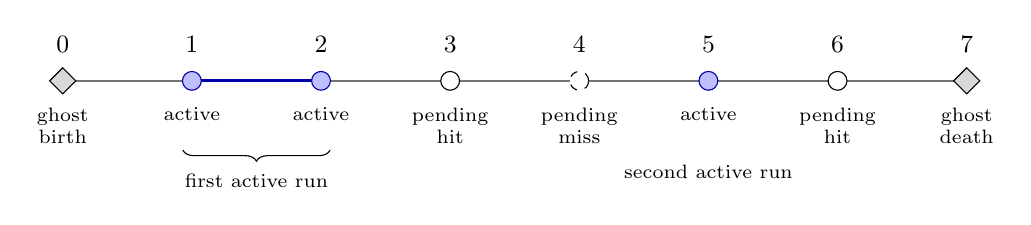
\begin{tikzpicture}[x=1.64cm,y=1cm,
  hit/.style={circle,draw=black,fill=white,inner sep=2.4pt},
  active/.style={circle,draw=blue!65!black,fill=blue!25,inner sep=2.4pt},
  ghost/.style={diamond,draw=black,fill=black!15,inner sep=2.4pt}]
\draw[thick,black!55] (0,0)--(7,0);
\draw[very thick,blue!65!black] (1,0)--(2,0);
\foreach \j in {0,...,7}
  \node[font=\small,above] at (\j,.23) {$\j$};
\node[ghost] at (0,0) {};
\node[active] at (1,0) {};
\node[active] at (2,0) {};
\node[hit] at (3,0) {};
\node[circle,draw=black,dashed,fill=white,inner sep=2.4pt] at (4,0) {};
\node[active] at (5,0) {};
\node[hit] at (6,0) {};
\node[ghost] at (7,0) {};
\node[font=\scriptsize,align=center,below] at (0,-.22) {ghost\\birth};
\node[font=\scriptsize,below] at (1,-.22) {active};
\node[font=\scriptsize,below] at (2,-.22) {active};
\node[font=\scriptsize,align=center,below] at (3,-.22) {pending\\hit};
\node[font=\scriptsize,align=center,below] at (4,-.22) {pending\\miss};
\node[font=\scriptsize,below] at (5,-.22) {active};
\node[font=\scriptsize,align=center,below] at (6,-.22) {pending\\hit};
\node[font=\scriptsize,align=center,below] at (7,-.22) {ghost\\death};
\draw[decorate,decoration={brace,mirror,amplitude=4pt}]
  (.93,-.88)--(2.07,-.88)
  node[midway,below=5pt,font=\scriptsize] {first active run};
\node[font=\scriptsize,below] at (5,-.95) {second active run};
\end{tikzpicture}
\caption{A schematic lifespan of a prime from group $i$.
All active visits and both ghost endpoints have its common line;
the pending visit at $4$ misses that line. The line contributes
$1/(p+1)$ once. After extracting $b'_p$, the ghost signs,
pending-hit damping, and active-run normalizations give the weight
$\eta'_0\eta'_7q_3q_6 V_i^{-2}/((p+1)b'_p)$.
The two powers of $V_i^{-1}$ count active runs, not active visits.}
\label{fig:lifespan}
\end{figure}


\subsection{The symmetric memory space and its operations}

We realize the preceding expansion by storing each pending prime
together with its line. A later active run retrieves that stored pair,
instead of paying for a new line. The following measures and transfer
factors are chosen to reproduce \eqref{mem:run-charge}.

Let $\mathcal Z$ be the finite set of primitive integer vectors in the
tube which satisfy the fixed-root box condition; it has counting
measure. An active list is an ordered $M$-tuple in each group, endowed
with measure $\bigotimes_i\nu_i^{\otimes M}$. The underlying list space
allows repetitions. Distinctness within physical lists and the other
local restrictions will be imposed in the operators.

A memory particle in group $i$ consists of a prime and an anchor,
\begin{equation}\label{mem:particle-space}
 \mathcal X_i=\{(p,\ell):p\in\mathcal P_i,
                 \ \ell\in\mathbb P^1(\mathbb F_p)\},\qquad
 \lambda_i(p,\ell)=\nu_i(p).
\end{equation}
The line coordinate has counting measure, not uniform probability
measure. In particular, anchoring a particle at $[z]_p$ leaves the
prime measure $\nu_i(p)$, without another factor $1/(p+1)$. A particle
\emph{hits} $z$ when its anchor equals $[z]_p$.

For a vector of memory sizes $\boldsymbol k=(k_1,\ldots,k_K)$,
use symmetric functions of the $k_i$ particles in each group and the
measure $\lambda_i^{\otimes k_i}/k_i!$. The Hilbert space is
\begin{equation}\label{mem:hilbert-space}
 \mathscr H=
 \ell^2(\mathcal Z)\otimes
 L^2\!\left(\bigotimes_i\nu_i^{\otimes M}\right)
 \otimes\bigotimes_{i=1}^K
 \left(\bigoplus_{k_i\ge0}
 L^2_{\mathrm{sym}}\!\left(\mathcal X_i^{k_i},
                   \frac{\lambda_i^{\otimes k_i}}{k_i!}\right)\right).
\end{equation}
Products and sums of the operators below use the row convention:
the input state is fixed, choices leading to output states are summed,
and the resulting operator acts on a test function at the output.
Let $\mathbf b$ be one when $z=e_1$ and memory is empty, and zero
otherwise; it is independent of the active lists. By
\eqref{mem:measure-masses},
\begin{equation}\label{mem:boundary-norm}
 \norm{\mathbf b}^2=\prod_i s_i^M
   =\exp\!\left(O_K\!\left(\frac{M(N+1)}{p_{\min}}\right)\right)
   =1+o(1).
\end{equation}

Fix once and for all
\begin{equation}\label{mem:rho}
 0<\rho<1,\qquad \rho^2>\sqrt q.
\end{equation}
The ghost operation $\mathcal G_j$ leaves the position and active list
unchanged. Independently in each group it first chooses a subset of
the indexed pending particles which hit the current position and
deletes them, paying $-\eta'_j/\rho$ per deletion. Each surviving hit
pays $q_j/\rho^2$. It then appends an ordered batch of $l\ge0$ primes,
integrated with measure $\nu_i^{\otimes l}/l!$, anchored at the current
lines, and with coefficient $(-\eta'_jV_i/\rho)^l$.
The divisor $l!$ makes the batch an unordered birth set when the primes
are distinct; the ordered integral will also be useful after that
restriction is removed.

The edge $\mathcal E_j$ retains the geometric multiplier in
\eqref{eq:det-kernel}, or its adjoint according to the alternating
physical path, but removes its $\omega$-damping and its active
divisibility tests. It replaces target unshared counting and
normalization by the following operations between the same endpoint
slot symmetrizations.
\begin{enumerate}[label=(\roman*)]
 \item Pay $\rho$ for every old pending particle which hits the source
 $z$. Choose a subset of the unshared source slots to store in memory,
 anchored at $[z]_p$, and drop the other unshared source slots. Copy the
 shared $J$ slots in each group.
 \item Choose a target position $z'$ and its unshared label in each
 group. A subset of these slots is filled by promoting indexed old
 particles which hit $z'$, removing them from memory and paying
 $1/V_i$ per promotion in group $i$. Particles just stored on this edge
 cannot be promoted on the same edge. Every other unshared target slot
 is filled by an independent $\nu_i$ draw.
 \item Pay $\rho$ for every particle remaining in memory which hits
 $z'$, including newly stored particles. Impose the physical endpoint
 list restrictions, the cross-edge ban, the pad dyad, all good-state
 tests and geometric cutoffs, using the actual source and target label
 products.
\end{enumerate}
Positions are always summed with counting measure. Since the real
root matrix has determinant one, its edge determinant is
$\det(z,z')$.

For the moment impose also that all \emph{performed births} have
globally distinct prime values. Births comprise initial active
entries, fresh target entries, and ghost creations. This is a
restriction on the fully expanded history, and is not claimed to be
a local projection on $\mathscr H$. Then the independent-line path sum,
divided by its extracted baseline, is exactly
\begin{equation}\label{mem:operator-history}
 \inner{\mathbf b}
 {\mathcal G_0\mathcal E_0\mathcal G_1\cdots
  \mathcal E_{N-1}\mathcal G_N\mathbf b},
 \qquad\text{with global birth distinctness imposed.}
\end{equation}
Here equality refers to the choice-by-choice expansion of the right
side. To verify it, a shared prime continues with the same line:
$p\mid D$ implies $\det(z,z')=0\pmod p$, and primitivity implies
$[z]_p=[z']_p$. A prime leaving activity either terminates there or is
stored. If it is used again, global birth distinctness forces its
promotion from that stored particle. Ghost creations and deletions
are exactly the optional endpoints of
\eqref{mem:orphan-identity}--\eqref{mem:suffix}.

At an internal pending hit, the incoming edge, ghost survival, and
outgoing edge give
\begin{equation}\label{mem:rho-cancellation}
 \rho\,(q_j/\rho^2)\,\rho=q_j.
\end{equation}
At a ghost birth the creation coefficient and outgoing hit factor
give $-\eta'_jV_i$; at termination the incoming hit factor and deletion
give $-\eta'_j$. There are no unmatched factors at $0,N$, because memory
starts and ends empty. An active birth has measure
$\nu_i(p)=((p+1)b'_p)^{-1}V_i^{-1}$, a ghost birth has prime measure
$V_i\nu_i(p)=((p+1)b'_p)^{-1}$ after this cancellation, and each
promotion pays $V_i^{-1}$. These are exactly the factors in
\eqref{mem:run-charge}: each new active run contributes $V_i^{-1}$,
while the lifespan has only one line-probability factor.
Conversely a compatible primewise lifespan determines all these
choices: store on leaving any nonfinal active run, promote on entering
the next, and create or terminate at its specified ghost endpoints.
The factorial birth integral counts its unordered ghost birth set
once. This proves the identity, including primes which leave and
later re-enter activity.

\subsection{Truncation and adjoints}

Let $B=\lceil L^2\rceil$ and let $\Pi_B$ restrict total memory size to
at most $B$. We may insert $\Pi_B$ before and after every operation in
\eqref{mem:operator-history}, with error
\begin{equation}\label{mem:truncation-error}
 O_A(L^{-AN})\qquad\text{for every fixed }A>0.
\end{equation}
This assertion is made while births are still globally distinct.
There are at most $KN$ stores in a history. A history reaching memory
size greater than $B$ has therefore had at least $B-KN$ ghost births.
Insert a factor two at each ghost birth in an absolute majorant.
For a prime active somewhere, there are at most $(N+2)^2$ possible
ghost endpoint pairs. There are $O_K(M+N)$ such primes along a fixed
active path. For a never-active prime, fixing its earlier ghost endpoint
and summing its possible later endpoints costs $O_q(1)$: successive
later endpoints with the required line acquire successive internal
factors at most $\sqrt q<1$. Summing the earlier endpoint gives a
total $O_q((N+1)/p)$ for the absolute ghost-only contribution, including
the inserted factor two. Consequently the product of all never-active
prime costs is $\exp(O_K(N+1))$.

The extracted baseline and its reciprocal have logarithms
$O_K(N+1)$, by \eqref{mem:baseline} and the bounded reciprocal prime
sums. The path and label enumeration used in the root replacement
costs $\exp(O_K(L^{.73}))$; multiplying by the active endpoint choices
and the preceding absolute costs gives, with room to spare,
$\exp(O_K(L^{.74}))$. Removing the inserted factors on the omitted
histories gives the upper bound
\[
 2^{-B+KN}\exp(O_K(L^{.74})),
\]
which proves \eqref{mem:truncation-error}.

We next omit global birth distinctness and work on
$\mathscr H_B=\Pi_B\mathscr H$. The resulting signed norm estimates
apply only to the unrestricted history; we will restore distinctness
by an exact expansion in equality constraints. Repeated pending values
are now permitted. All deletion and promotion choices remain choices
of indices, so that the following
adjoint identities hold also in their presence.

Suppose $a$ particles are deleted from a memory list of size $k+a$.
For an unordered ghost deletion batch its indexed choices and the
factorial memory measure give
\begin{equation}\label{mem:ghost-factorial}
 \frac{\binom{k+a}{a}}{(k+a)!}=\frac{1}{k!a!}.
\end{equation}
Its anchors are forced by the hit condition, leaving exactly the
$\nu_i$ integrations. A fresh ghost batch has the same factorial
integral. Interchanging the deleted and appended batches therefore
gives the adjoint ghost operation: its deletion coefficient is
$-\eta'_jV_i/\rho$ and its creation coefficient is $-\eta'_j/\rho$;
the surviving-hit multiplier stays $q_j/\rho^2$.

For retrieval into $a$ prescribed ordered active slots the corresponding
identity is
\begin{equation}\label{mem:edge-factorial}
 \frac{\binom{k+a}{a}a!}{(k+a)!}=\frac{1}{k!}.
\end{equation}
The retrieved anchors again force one line and leave $\nu_i$ prime
integrations. Newly stored particles get those same prime measures
from their source active entries. Thus at two fixed positions the
joint measure of all source and target active entries and all memory
coordinates is unchanged on exchanging stores and promotions. The
factor $1/V_i$ on a forward promotion stays on that transfer, becoming
a reversed store factor; this is a bounded factor. The two endpoint
$\rho$ factors exchange roles. Summing over the two positions
preserves the equality because their measure is counting measure.
Slot symmetrizations are self-adjoint averages, and all endpoint and
edge restrictions transpose with the kernel. These observations
prove the adjoint rules even when list restrictions depend jointly
on both positions.

For later use, a local choice multiplier of modulus at most one may be
inserted provided it is equivariant under simultaneous permutations of
the old memory coordinates and the selected deletion or promotion
indices. The indexed choice sum then preserves symmetry in the old
particles. In a ghost birth integral, a multiplier depending on the
ordered fresh batch is averaged over permutations of that batch when
acting on symmetric test functions. This leaves the integral unchanged,
keeps its modulus at most one, and retains the factor $1/l!$. These
modified operations therefore act on the same symmetric spaces. In
both adjoint directions they are dominated in absolute value by the
positive kernels obtained by summing the absolute values of the
unmodified operation-choice coefficients. An arbitrary multiplier depending
on an old particle's index alone need not preserve symmetry and is not
allowed here.

\subsection{Absolute bounds for ghosts and edges}

Call an edge \emph{clean} if it stores and promotes no particle, and
\emph{dirty} otherwise. A clean edge draws all unshared target labels
freshly, and its signed minor-arc kernel will give cancellation.
For a dirty edge the good-state tests instead make an absolute row or
column sum small. We first bound the ghosts and record crude edge
bounds, then prove these two kinds of small edge estimate.

For a state with total pending size $k_{\mathrm{tot}}$ use the positive
Schur weight
\begin{equation}\label{mem:schur-weight}
 w=v_0^{k_{\mathrm{tot}}},
\end{equation}
where $v_0$ is a sufficiently large fixed constant. A weighted row
bound $R$ means that the absolute row sum against output weight is
at most $R$ times input weight; the analogous bound for the adjoint is
the weighted column bound $C$. Weighted Schur gives norm at most
$\sqrt{RC}$. Restrictions by $\Pi_B$ can only decrease these absolute
sums.

In one group with $h$ pending hits, the ghost row bound, divided by
the input weight, is
\begin{equation}\label{mem:ghost-row}
 \exp\!\left(\frac{v_0\eta'_jV_i s_i}{\rho}\right)
 \left(\frac{q_j}{\rho^2}+\frac{\eta'_j}{\rho v_0}\right)^h.
\end{equation}
The exponential sums fresh births; the power sums deletion or survival
of each old hit. The adjoint bound is
\begin{equation}\label{mem:ghost-column}
 \exp\!\left(\frac{v_0\eta'_j s_i}{\rho}\right)
 \left(\frac{q_j}{\rho^2}+\frac{\eta'_jV_i}{\rho v_0}\right)^h.
\end{equation}
Since $q_j\le\sqrt q<\rho^2$ and the $V_i$ are bounded above and below,
one fixed $v_0$ makes both parentheses at most one, for all $i,j$ and
large $x$. Multiplication over the fixed groups proves
\begin{equation}\label{mem:ghost-norm}
 \norm{\mathcal G_j}_{\mathscr H_B\to\mathscr H_B}\le C_K,
\end{equation}
with the same absolute row and column bounds under the bounded choice
modifications just described.

For the crude edge bounds fix the source $z$ and choose an integral
complement $w_z$ with $\det(z,w_z)=1$. Write
\begin{equation}\label{mem:neighbor}
 z'=j_1w_z+h z,\qquad j_1=\det(z,z'),\qquad
 \left|h+j_1\frac{\tau(w_z)}{\tau(z)}\right|\le16.
\end{equation}
The last inequality follows from $\tau(z')/\tau(z)$ lying in the
fixed box range. Enlarging its absolute constant would have no effect
on any argument below. For fixed source, labels, and determinant
$j_1$, this permits $O(1)$ targets. In the raw determinant part
$j_1=D(b-a)$ is fixed. In the comparison part $j_1=Dt$ has $O(Y)$
possibilities, and its multiplier is at most
\begin{equation}\label{mem:major-absolute}
 C\abs{\mathfrak M}\ll \frac{L^{3A_0}}{Y}.
\end{equation}
The masses of all fresh label draws are bounded by $C_K$.
There are at most $C_KB^K$ indexed promotion choices. Store subsets,
Schur weight ratios and $V_i$ factors cost $C_K$. Source and target
symmetrizations are probability averages. Using the adjoint
calculation for columns, we obtain a constant $C=C(K,A_0,q)$ such that
\begin{equation}\label{mem:edge-crude}
 R(\mathcal E_j),\ C(\mathcal E_j)
       \le C_K B^K(1+L^{3A_0})\le L^C.
\end{equation}
This holds for arbitrary multipliers of modulus at most one on the
choices. It also holds after fixing any or all fresh prime values,
with their measures left outside the bound. This uniformity will
preserve the cost of a forced prime atom in the birth-distinctness
argument.

\subsection{The lattice box and the clean signed norm}

We first extract a geometric consequence of the first good-state
test. Partition $\mathcal Z$ by intervals of length $H=d_0Y$ for
$z_2/\tau(z)$. The identity
\[
 \frac{z'_2}{\tau(z')}-\frac{z_2}{\tau(z)}
      =\frac{\det(z,z')}{\tau(z)\tau(z')}
\]
shows that an edge connects only cells whose indices differ by a
bounded amount. At fixed shared list, hence fixed squarefree product
$D$, partition further by the tuple $([z]_p)_{p\mid D}$. An edge
preserves this tuple. The resulting operator is a sum over a bounded
number of cell-index shifts of direct sums of blocks. It suffices to
bound each block uniformly.

Choose a relevant good source $z$ in one such pair of cells and a
complement $w_z$ as in \eqref{mem:neighbor}. All vectors in either cell
with the specified line tuple belong to the lattice
\[
 \Lambda=\mathbb Z z+\mathbb Z D w_z.
\]
Indeed, on writing a vector as $h z+jw_z$, equality of the projective
lines modulo every $p\mid D$ implies $p\mid j$; squarefreeness gives
$D\mid j$. Its coordinates $(h,l)$ in this lattice satisfy
\begin{equation}\label{mem:sheared-box}
 |l|\ll Y,\qquad |h+l\alpha|\ll1,
 \qquad \alpha=D\frac{\tau(w_z)}{\tau(z)}.
\end{equation}
The $l$ bound follows from the cell separation and $D\asymp d_0$;
the other follows from the box condition.

The image of this integer lattice under
$(h,l)\mapsto(h+l\alpha,l/Y)$ has covolume $1/Y$.
Let $\lambda$ be the length of its shortest nonzero vector. If
$\lambda<Y^{-.8}$, its second coordinate gives
$0<|l|<Y^{.2}$, and its first gives
$\|l\alpha\|<Y^{-.8}<Y^{-.7}$; $l=0$ is impossible for a nonzero
vector this short. This contradicts the first good-state test, since
$\tau(w_z)/\tau(z)$ is a lift of $r_{gz}$. Thus
$\lambda\ge Y^{-.8}$. Dirichlet's elementary pigeonhole approximation,
using denominators at most $\lceil\sqrt Y\rceil$, gives
$\lambda\ll Y^{-.5}$.

A shortest vector is primitive in the lattice, so complete it to a
basis. Subtract a multiple of the first vector from the second to
make its parallel component at most $\lambda/2$. Its perpendicular
component is $1/(Y\lambda)$; since $\lambda^2\ll1/Y$, its length is
$O(1/(Y\lambda))$. Inverting this basis on the bounded region in
\eqref{mem:sheared-box} puts all relevant vectors in a centered
coordinate box with side parameters $O(1/\lambda)$ and $O(Y\lambda)$.
Choose its orientation positively. Enlarging constants, the box has
parameters $A',B'$ satisfying
\begin{equation}\label{mem:lattice-shape}
 A'B'\ll Y,\qquad Y^{.1}\le A',B'\le Y^{.9}.
\end{equation}
The change of integer basis has determinant one, so that
$\det(z,z')/D$ is the ordinary determinant of their new integer
coordinates. This proof applies unchanged for a continuous root:
the tested quantity $r_{gz}$ is still
$\tau(w_z)/\tau(z)\bmod1$.

For a clean edge, before the slot symmetrizations, condition on the
shared list and all pending particles. They are unchanged by the central
operation. Its remaining
pending-hit factors are diagonal contractions at the two endpoints.
We may omit the extra cross-edge ban at a norm cost smaller than any
power of $L^{-1}$. In fact, keeping distinctness of each full active
list, a forbidden coincidence requires one of the fresh labels to
equal a fixed source label, costing at most
$C_KM\sup_{i,p}\nu_i(p)$. After the labels are fixed,
\eqref{mem:neighbor} and \eqref{mem:major-absolute} give an absolute
row bound $C_K L^{3A_0}$; the same argument for the adjoint gives the
column bound. Equation~\eqref{mem:measure-masses} proves the claimed
negligible norm cost.

Inside a lattice block, the unshared ordered list, containing one
prime from each disjoint band, is uniquely determined by its product
$b$. Its measure is
\begin{equation}\label{mem:product-mass}
 m(b)=\prod_{i=1}^K\nu_i(p_i)\le\frac{C_K}{Y}
 \quad\text{when }\eta(b/Y)\ne0.
\end{equation}
Conjugation from $L^2(m)$ to counting measure inserts
$\sqrt{m(b)m(a)}$. Consequently the clean norm is at most $C_K$ times
the norm of the following operator on the integer box in
\eqref{mem:lattice-shape} and an unrestricted integer product variable:
\begin{equation}\label{mem:clean-kernel}
 \frac1Y\psi\!\left(\frac{\det(\boldsymbol h,\boldsymbol l)}Y\right)
 \int_{\mathbb T\setminus\mathfrak M}
 \e\!\left(\theta
      (\det(\boldsymbol h,\boldsymbol l)-b+a)\right)\,\dd\theta.
\end{equation}
Here $\mathbb T=\mathbb R/\mathbb Z$. Extending the product variable
means composing with extension by zero and restriction. All actual
product supports, full-list restrictions, goodness tests, cutoff
factors, and the bounded square-root factors from
\eqref{mem:product-mass} are endpoint diagonal multipliers. The factor
$d_0/D$ is bounded. Thus none of these operations increases the bound
except by $C_K$. We use the transposed conjugate kernel on a reversed
edge.

Fourier transformation in the unrestricted integer product variable
diagonalizes its convolution: for each
$\theta\in\mathbb T\setminus\mathfrak M$ the fiber is the determinant
exponential matrix with its smooth cutoff, divided by $Y$. If
$\widehat\psi(u)=\int_{\mathbb R}\psi(t)\e(-ut)\,\dd t$, then
\begin{equation}\label{mem:cutoff-fourier}
 \psi\!\left(\frac{\det(\boldsymbol h,\boldsymbol l)}Y\right)
 \e\bigl(\theta\det(\boldsymbol h,\boldsymbol l)\bigr)
 =\int_{\mathbb R}\widehat\psi(u)
   \e\bigl((\theta+u/Y)\det(\boldsymbol h,\boldsymbol l)\bigr)
   \,\dd u.
\end{equation}
The density $\widehat\psi$ decreases faster than any inverse power.

For $|u|\le L^{A_0}/2$, put $\vartheta=\theta+u/Y$. Dirichlet
approximation with $Q=\lceil Y/L^{A_0}\rceil$ gives a reduced
$c/d$ such that
\begin{equation}\label{mem:dirichlet-minor}
 L^{A_0}<d\le Q,\qquad
 \left|\vartheta-\frac cd\right|
        \le\frac1{dQ}\le\frac1{d^2}.
\end{equation}
Indeed $d\le L^{A_0}$ would put $\theta$ within
$\tfrac32L^{A_0}/Y$ of a rational of allowed denominator, contrary
to the definition of $\mathfrak M$ with radius $2L^{A_0}/Y$.

For completeness, let $T_{A',B'}(\vartheta)$ have entries
$\e(\vartheta hk)$ for integer $|h|\ll A'$, $|k|\ll B'$.
Its Gram matrix and the geometric-sum estimate give
\begin{equation}\label{mem:bilinear-gram}
 \norm{T_{A',B'}(\vartheta)}^2
 \ll\sum_{|h|\ll A'}\min\!\left(B',\frac1{\|h\vartheta\|}\right)
 \ll (A'/d+1)\bigl(B'+d\log(2d)\bigr).
\end{equation}
In the term $h=0$ the minimum is interpreted as $B'$. To justify the
last inequality, split the $h$ interval into blocks of length at most
$d/2$. For two different indices in a block, reduction of $c/d$ and
the error in \eqref{mem:dirichlet-minor} separate their fractional
parts by at least $1/(2d)$. Ordering their distances to the nearest
integer bounds each block by
$O(B'+d\sum_{1\le j\le d}j^{-1})$.

Up to a permutation of columns, the determinant matrix
$\e(\vartheta(h_1l_2-h_2l_1))$ is the tensor product of
$T_{A',B'}(\vartheta)$ and its transposed conjugate. Its norm is
therefore the squared norm in \eqref{mem:bilinear-gram}. After division
by $Y$, \eqref{mem:lattice-shape} implies the bound
\begin{equation}\label{mem:minor-decay}
 \frac{\norm{(\e(\vartheta\det(\boldsymbol h,\boldsymbol l)))}}Y
 \ll \frac1d+Y^{-.1}\log(2Y)
          +\frac{d\log(2d)}Y
 \ll_K L^{.2-A_0}+Y^{-.1}\log(2Y).
\end{equation}
For the complementary Fourier tail in \eqref{mem:cutoff-fourier},
the trivial matrix norm is $O(A'B')=O(Y)$, so rapid decay of
$\widehat\psi$ gives any required negative power of $L$. Combining
the direct sums of cell blocks and the endpoint symmetrizations,
we conclude that, for any fixed $G>0$, choosing $A_0$ sufficiently
large in terms of $G$ gives
\begin{equation}\label{mem:clean-bound}
 \norm{\mathcal E_j^{\mathrm{clean}}}\le L^{-G}
\end{equation}
for large $x$, with an arbitrarily fixed margin in the exponent.
Constants depending on the later fixed value of $K$ are absorbed by
that margin and the threshold for $x$.

\subsection{Dirty raw edges: the two Schur sides}

Fix the set $S$ of stored groups and the set $I$ of promoted groups.
There are at most $4^K$ choices, a constant. All store and promotion
coefficients and the ratio of Schur weights cost $C_K$.

If $I=\varnothing$, the weighted raw row bound is $C_K$, independently
of $B$. For each source omission tuple, sample the fresh target label
in every group and use \eqref{mem:neighbor} with its fixed determinant.
There are no pending-index choices. The source symmetrization averages
the omission tuples and thus does not multiply their number. This
argument allows arbitrary $S$.

Suppose $I\ne\varnothing$ and put $i_* =\max I$. Fix the source state
and sample the fresh target labels in the groups outside $I$, with
product $T_f$. Their product law $\nu$ is boundedly comparable to the
law $\mu$ in the second good-state test, by
\eqref{mem:measure-masses}. Outside an exceptional mass
$C_K\exp(-\tfrac14L^{a_{i_*}})$, that test supplies its asserted phase
separation. Fix one old index for promotion in group $i_*$; there are
at most $B$ such indices, and write its prime and anchor as
$(p_*,\ell_*)$. Let $Z$ be the product of the other promoted numeric
primes and let $P_{\mathrm{full}}$ be the product of the complete source
active list. The raw determinant equation is
\begin{equation}\label{mem:dirty-determinant}
 j_1=P_{\mathrm{full}}-Dp_*ZT_f.
\end{equation}
The ban excludes $p_*$ from the entire source list. Thus
$j_1\equiv P_{\mathrm{full}}\ne0\pmod{p_*}$, independently of the
omission tuple and of $Z$.

In \eqref{mem:neighbor} the line condition
$[j_1w_z+hz]_{p_*}=\ell_*$ is either impossible or fixes a single
residue $h=h_*\pmod{p_*}$. To see uniqueness, in the basis
$(z,w_z)$ the second coordinate $j_1$ is nonzero modulo $p_*$;
therefore its projective line determines the first coordinate
uniquely. This residue depends on the fixed index and
$P_{\mathrm{full}}$, but not on $D,Z$. Substitution in
\eqref{mem:neighbor}, using the real lift
$r_z^*=\tau(w_z)/\tau(z)$, yields
\begin{equation}\label{mem:anchor-congruence}
 \left\|DZ T_f r_z^*
       -\frac{P_{\mathrm{full}}r_z^*+h_*}{p_*}\right\|
       \le\frac{16}{p_*}.
\end{equation}
The phase separation is $100e^{-L^{a_{i_*}}}$, whereas the diameter
of the interval in \eqref{mem:anchor-congruence} is at most
$32/p_*\le32e^{-L^{a_{i_*}}}$. Hence at most one distinct integer
$DZ$ is possible.

This also determines $D$ and $Z$ separately. All prime factors of $D$
are source labels and all prime factors of $Z$ are excluded from the
source list by the ban. Their prime factorizations therefore separate
unambiguously. Because the source list is distinct, $D$ determines
which single label was omitted in every group. Under source
symmetrization this one numeric omission tuple has mass exactly
$M^{-K}$. It is an average over tuples, including over their internal
orders, rather than an unnormalized sum. The disjoint prime bands
also make $Z$ determine each other promoted numeric prime.

The labels now fix $j_1$, so there are $O(1)$ target positions. At any
one of them, multiplicities among the remaining promoted indices are
absorbed by the outgoing pending damping. If a group has $h$ old
particles hitting that target, the choice of one eligible index and
the damping of all other old hits cost at most
\begin{equation}\label{mem:index-damping}
 h\rho^{h-1}\le\sup_{n\ge1}n\rho^{n-1}<\infty.
\end{equation}
This remains true for repeated numeric values and repeated anchors.
Additional newly stored hits only decrease the factor. Applying this
in each of the other promoted groups costs $C_K$. For the exceptional
fresh draws use the crude $B^K$ count and
\eqref{mem:neighbor}. We obtain the weighted raw row bound
\begin{equation}\label{mem:epsilon}
 \varepsilon_K=C_K\left(\frac{B}{M^K}
                         +B^K e^{-cL^{.1}}\right)
 \qquad(I\ne\varnothing).
\end{equation}

Reversal exchanges $S$ and $I$ by \eqref{mem:edge-factorial}, changes
only bounded $V_i$ factors, and retains both good-state tests and the
ban. Its raw determinant equation, with the reversed sign, again has
source full product minus $D$ times the target unshared product.
The preceding argument therefore gives the following complete table.
Every entry includes the fixed $C_K$ factors.
\begin{center}
\begin{tabular}{cccc}
\toprule
Stored groups $S$ & Promoted groups $I$ & Weighted row & Weighted column\\
\midrule
$\varnothing$ & $\varnothing$ & $C_K$ & $C_K$\\
$\varnothing$ & nonempty & $\varepsilon_K$ & $C_K$\\
nonempty & $\varnothing$ & $C_K$ & $\varepsilon_K$\\
nonempty & nonempty & $\varepsilon_K$ & $\varepsilon_K$\\
\bottomrule
\end{tabular}
\end{center}
The first row is only an absolute estimate; its signed estimate is
\eqref{mem:clean-bound}. Once $K$ is large enough that
$\varepsilon_K\le1$, weighted Schur bounds the sum of the three dirty
raw cases by
\begin{equation}\label{mem:raw-dirty-norm}
 C_K\sqrt{\varepsilon_K}
 \le C_K L^{1-.005K+o(1)}+O_A(L^{-A})
 \quad\text{for every fixed }A.
\end{equation}
The bounded entry opposite a small Schur entry is essential here: it
contains no factor $B^K$. Thus making $.005K$ larger than a prescribed
constant purchases that constant in log decay. All remaining
$K$-dependence in this estimate is a fixed multiplicative constant.

\subsection{Dirty comparison edges}

Use the supremum \eqref{mem:major-absolute}, discarding its dependence
on the target unshared labels. Fix a source omission tuple, hence
$D$, and suppose $I\ne\varnothing$. A promoted old index with prime
$p$ requires one specified projective line at the target. By the ban,
$p\nmid D$. The lattice basis used to obtain
\eqref{mem:lattice-shape} has determinant $D$ in the original integer
coordinates and is therefore invertible modulo $p$. The prescribed
line is consequently one nonzero homogeneous linear congruence in
the two box coordinates.

For a box of sides $A',B'$, the number of solutions of such a
congruence is
\begin{equation}\label{mem:line-count}
 O\!\left(\frac{A'B'}p+\max(A',B')\right)
 \ll Y\left(\frac1p+\frac1{\min(A',B')}\right).
\end{equation}
If the coefficient of the shorter coordinate is nonzero, fix the
other coordinate and count its solutions in that shorter interval.
If that coefficient vanishes, the congruence restricts the longer
coordinate instead; the same displayed upper bound follows. We have
included vectors divisible by $p$ in this count, which only increases
it.

For each source only a bounded number of neighboring cell blocks
occurs. Take the union over at most $B$ old indices in one promoted
group. The other index choices can be bounded by $B^{K-1}$, or by
\eqref{mem:index-damping}. Sum the fresh prime masses and the source
omission average. Equations \eqref{mem:major-absolute},
\eqref{mem:lattice-shape}, and \eqref{mem:line-count} give a row bound
\begin{equation}\label{mem:comparison-small}
 \zeta_K
   :=C_K L^{3A_0}B^K\left(p_{\min}^{-1}+Y^{-.1}\right),
 \qquad \zeta_K=O_A(L^{-A})
 \quad\text{for every fixed }A.
\end{equation}
All parameters $K,A_0$ are fixed in the last assertion. The opposite
Schur side is at most $L^C$ by \eqref{mem:edge-crude}. For a store-only
piece apply the same argument to the adjoint; with both stores and
promotions it applies to both sides. For clarity the comparison
counterpart of the dirty table is
\begin{center}
\begin{tabular}{cccc}
\toprule
Stored groups $S$ & Promoted groups $I$ & Weighted row & Weighted column\\
\midrule
$\varnothing$ & nonempty & $\zeta_K$ & $L^C$\\
nonempty & $\varnothing$ & $L^C$ & $\zeta_K$\\
nonempty & nonempty & $\zeta_K$ & $\zeta_K$\\
\bottomrule
\end{tabular}
\end{center}
Weighted Schur makes every dirty comparison piece smaller than every
fixed negative power of $L$.

Choose $G>E_0+3$. First choose $A_0$ so that the clean argument gives
more than $G$ powers of decay, and then choose $K$ so that
$.005K>G+2$. Combining the clean, dirty raw, and dirty comparison
estimates, with their fixed finite sums, proves
\begin{equation}\label{mem:signed-edge}
 \norm{\mathcal E_j}_{\mathscr H_B\to\mathscr H_B}\le L^{-G}
\end{equation}
before global birth distinctness is restored. If desired all strict
inequalities here can be enlarged by one to absorb the constants.
The crude exponent $C(K,A_0,q)$ in \eqref{mem:edge-crude} has not
entered the choice needed in \eqref{mem:raw-dirty-norm}.

\subsection{Restoring global birth distinctness}

The contractions just proved did not require globally distinct births.
We now restore that condition exactly. A union bound over one repeated
prime would not suffice against the absolute cost of a long path;
we instead separate equality constraints by their rank.

Allocate a finite ordered set $\mathcal B$ of potential birth
addresses as follows: the $KM$ initial slots; the $K$ canonical target
slots at each edge, before its final symmetrization; and $B$ ordered
fresh-batch indices per group at each ghost operation. The truncation
ensures that a ghost batch has length at most $B$. Each address has
a local \emph{performed flag}: at an edge it is performed exactly if
that slot is filled freshly, and in a ghost batch exactly if its index
does not exceed the batch length. Initial addresses are always
performed. Thus
\begin{equation}\label{mem:address-count}
 Q_{\mathrm{birth}}:=\abs{\mathcal B}
       \le KM+KN+K(N+1)B=L^{O(1)}.
\end{equation}
Order these addresses chronologically, with a fixed order within
each operation.

Let $\mathcal C$ be a collection of disjoint nonsingleton subsets of
$\mathcal B$. For each block $C\in\mathcal C$ require that every
address is performed and that their prime values are equal. Denote
this event by $E_C$. Then the exact distinctness indicator is
\begin{equation}\label{mem:partition-identity}
 \1_{\text{distinct performed birth values}}
 =\sum_{\mathcal C}
       \prod_{C\in\mathcal C}(-1)^{|C|-1}(|C|-1)!
       \prod_{C\in\mathcal C}\1_{E_C}.
\end{equation}
One proof expands the right side as the sum of signs of all
permutations of the performed addresses which preserve their values:
a nontrivial cycle on $C$ has sign $(-1)^{|C|-1}$ and there are
$(|C|-1)!$ such cycles. In each equal-value class of size at least two
the signs of permutations sum to zero, and for a singleton they sum
to one. Unperformed addresses cannot occur in a nontrivial cycle,
which is exactly enforced by the flags.

Define the rank
\begin{equation}\label{mem:rank-definition}
 r(\mathcal C)=\sum_{C\in\mathcal C}(|C|-1).
\end{equation}
A rank-$r$ collection involves at most $2r$ addresses. Its total
absolute coefficient mass, summed over all collections of that rank,
is at most
\begin{equation}\label{mem:rank-coefficients}
 Q_{\mathrm{birth}}^{2r}=L^{O(r)}.
\end{equation}
Indeed the coefficients count permutations with that cycle rank,
and each such permutation has a fixed canonical decomposition into
$r$ transpositions. Its ordered list of transpositions, drawn from
at most $Q_{\mathrm{birth}}^2$ possibilities, determines the
permutation.

We first bound a fixed system of equality constraints absolutely.
In each block choose its earliest address as pivot, and condition
chronologically on the entire earlier history and all known pivot
values. Each nonpivot performed birth must draw one prescribed prime.
By \eqref{mem:measure-masses} this costs an atom at most
\begin{equation}\label{mem:atom}
 \Delta:=\sup_{i,p}\nu_i(p)\le C_K e^{-L^{.1}}.
\end{equation}
If its prescribed value belongs to a wrong group, the term is zero.
No later endpoint conditioning is imposed in this absolute bound:
we drop the final return requirement and use weighted row iteration.
Thus dependence of intermediate positions on the earlier pivot
values cannot change the atom cost.

Here is the precise uniform estimate justifying that iteration.
For an edge with $s$ prescribed nonpivot fresh values, fix all fresh
values first. The possible target positions still number $O(1)$ in
the raw part or $O(Y)$ in the comparison part. The latter count is
compensated by \eqref{mem:major-absolute}. Consequently its weighted
absolute row is at most
\begin{equation}\label{mem:edge-atoms}
 C_K B^K(1+L^{3A_0})\Delta^s,
\end{equation}
uniformly in the input state and all fixed values. The remaining fresh
values have bounded total mass, and all local restrictions may be
discarded for this upper bound.

For a ghost in group $i$, set
$c_i=v_0\eta'_jV_i/\rho$. If $s$ specified ordered coordinates of
its new batch are prescribed, its birth row sum is at most
\begin{equation}\label{mem:ghost-atoms}
 \sum_{l\ge s}\frac{c_i^l\Delta^s s_i^{l-s}}{l!}
 \le(c_i\Delta)^s\exp(c_i s_i).
\end{equation}
The actual requirement that the batch reaches its largest named
index can only reduce this sum. Within a batch the earlier pivot
coordinates are integrated before the prescribed later ones, which
gives the same estimate. Deletion and survival have weighted factor
at most one by \eqref{mem:ghost-row}. Anchors add no factor $p+1$,
as their measure is counting measure. Initial slots have the same
single-atom estimate. Thus for each fixed rank-$r$ constraint system,
the absolute boundary contribution is at most
\begin{equation}\label{mem:rank-absolute}
 L^{C(N+1)}(C_K e^{-L^{.1}})^r,
\end{equation}
for a fixed $C=C(K,A_0,q)$. The boundary weight is one because memory
is empty; after dropping return, its terminal indicator is at most
the positive Schur weight, so the chronological row bounds apply.

Choose, after $C$ is fixed,
\begin{equation}\label{mem:rank-cutoff}
 r_0=\left\lceil C'\frac{N\log L}{L^{.1}}\right\rceil,
\end{equation}
with $C'$ sufficiently large. Combining
\eqref{mem:rank-coefficients} and \eqref{mem:rank-absolute}, and using
$\log Q_{\mathrm{birth}}=O(\log L)$, bounds all ranks $r\ge r_0$ by
\begin{equation}\label{mem:high-rank}
 L^{C(N+1)}\sum_{r\ge r_0}
   \bigl(C_K Q_{\mathrm{birth}}^2e^{-L^{.1}}\bigr)^r
 \le L^{-(E_0+2)N}.
\end{equation}
The series is geometric for large $x$. For example its ratio is at
most $e^{-L^{.1}/2}$, so choosing $C'/2>C+E_0+3$ suffices after
enlarging the threshold for $x$.

For ranks $r<r_0$, use signed contraction on most edges. If
$C=\{a_0,a_1,\ldots,a_s\}$ is one block, with earliest address $a_0$,
write its equality event by ordinary circle orthogonality as
\begin{equation}\label{mem:local-phases}
 \1_{E_C}
 =\left(\prod_{a\in C}\1_{a\ \mathrm{performed}}\right)
   \int_{\mathbb T^s}
      \prod_{h=1}^s
          \e\bigl(\theta_h(p_{a_h}-p_{a_0})\bigr)
      \,\dd\theta_1\cdots\dd\theta_s.
\end{equation}
When an address is unperformed the integrand is interpreted as zero;
no value is assigned to an unperformed birth. After the circle
variables are fixed, every phase is attached only to the operation
where its prime was created. In particular the pivot receives the
single local multiplier
$\e(-p_{a_0}\sum_h\theta_h)$. Its value need not be remembered through
later operations. Flags are local choice restrictions of modulus at
most one. An edge flag tests whether its slot is freshly drawn rather
than promoted; it does not distinguish old promotion indices. A ghost
flag tests whether its fresh batch reaches the specified address.
Thus these flags and birth-value phases satisfy the old-memory
equivariance condition stated after \eqref{mem:edge-factorial}.
For fixed circle variables, backward induction through the later
operations gives a symmetric continuation function. Averaging the
ghost-batch multiplier over its new coordinates consequently leaves
the full integral unchanged, without increasing its absolute kernel,
changing its factor $1/l!$, or modifying any later operation.

It follows that a rank-$r$ system modifies at most $2r$ operations,
and hence at most $2r$ edges. Initial phases change $\mathbf b$ by a
bounded multiplier and preserve \eqref{mem:boundary-norm}. Every
ghost, modified or not, has norm at most $C_K$; a modified edge has
norm at most $L^C$ by \eqref{mem:edge-crude}; all other edges retain
\eqref{mem:signed-edge}. For each fixed set of phases the boundary
matrix element is therefore at most
\begin{equation}\label{mem:low-rank-term}
 C_K^{N+1}\norm{\mathbf b}^2
       L^{-G(N-2r)} L^{2Cr}.
\end{equation}
Integration of phases does not increase this bound. As
$r_0/N=O(\log L/L^{.1})=o(1)$, summing
\eqref{mem:low-rank-term} with \eqref{mem:rank-coefficients} gives
\begin{equation}\label{mem:low-rank}
 \sum_{r<r_0}Q_{\mathrm{birth}}^{2r}
 C_K^{N+1}\norm{\mathbf b}^2 L^{-G(N-2r)+2Cr}
       \le L^{(-G+o(1))N}.
\end{equation}
This remains true even though $C$ depends on $K$: $K$ was fixed
before letting $x$ grow, and its crude exponent is paid on only
$o(N)$ edges.

Equations \eqref{mem:high-rank} and \eqref{mem:low-rank} bound
\eqref{mem:operator-history} with exact global birth distinctness,
uniformly in all archimedean root variables. Multiply back the
baseline, whose modulus is at most one. The root integral has bounded
mass. The error \eqref{mem:truncation-error} and the root-replacement
error are $O_A(L^{-AN})$ for arbitrary fixed $A$. Because
$G>E_0+3$, these margins absorb all constants and prove
\eqref{mem:moment-bound}. The passage from this moment to
\eqref{eq:det-pairing} was proved in the preceding section.

\subsection{Removing goodness and stripping the pads}

We complete the second assertion of
Proposition~\ref{prop:minor-moment}. First remove the good-state
projections from the endpoint pairing. The part where the source is
bad, and separately the part where the target is bad, may be
majorized absolutely; bound the endpoint coefficients by their
log-power suprema. Apply the single-edge version of the root
replacement. In the independent-line model, a shared prime requires
the same line at both positions, or contributes zero. Every distinct
prime in the union of the two active lists is charged exactly once
by $1/(p+1)$. The ban makes the union consist of $M+1$ distinct primes
per group. Its list normalization is $V_i^{-(M+1)}$, so summing these
probabilities over ordered union lists is at most
\begin{equation}\label{mem:one-edge-label-mass}
 \prod_{i=1}^K
 \left(\sum_{p\in\mathcal P_i}\frac1{V_i(p+1)}\right)^{M+1}
 \le1.
\end{equation}
We have dropped any incompatibilities for an upper bound. Damping
is also at most one on the physical states and may be discarded.

For fixed labels, \eqref{mem:neighbor} counts $O(1)$ raw targets;
the comparison target count is $O(Y)$ and is compensated by
\eqref{mem:major-absolute}. For every fixed source list, the set of
root ratios failing either good-state test has measure
$O(e^{-cL^{.1}})$ by Lemma~\ref{det:good-state}. This estimate
is uniform in the other root coordinates. The preceding target
counts hold for every ratio, so they may be integrated over that bad
set. Reversal proves the identical assertion for failure of target
goodness. Equation~\eqref{mem:one-edge-label-mass} then gives the
normalized pairing error
\begin{equation}\label{mem:goodness-error}
 O\!\left(UV L^{C_1+3A_0}e^{-cL^{.1}}\right)
       +O_A(UV L^{-A}),
\end{equation}
where $C_1$ comes from the endpoint suprema. The root-replacement
error can here be made smaller than every log power by its
single-edge estimate; this also handles the indicators of goodness
failure. Therefore removing the projections costs
$O_A(UV L^{-A})$ for every fixed $A$.

The endpoint vectors are invariant under permutations of their
lists. Hence the two slot symmetrizations disappear when the pairing
is expanded. Write the ordered pads as $p_{i,1},\ldots,p_{i,J}$ in
group $i$, with total product $D$. The remaining source and target
slots have products $b$ and $a$. The common state normalization and
the fresh-target normalization are
$\prod_i V_i^{-(J+2)}$. Divide the pairing for the dyad $d_0$ by
$d_0$. Its scalar multiplier becomes $1/D$, and the exact measure
identity is
\begin{equation}\label{mem:pad-measure}
 \frac1D\prod_{i=1}^K V_i^{-(J+2)}
   =\left(\prod_{i=1}^K\prod_{h=1}^J\mu_i(p_{i,h})\right)
      \prod_{i=1}^K V_i^{-2}.
\end{equation}
Thus the pads are independent ordered harmonic draws, and the
remaining factors are exactly the two unshared-list normalizations
in the expanded square. There is no factorial or $M$-dependent
normalization left over: the pads occupy prescribed ordered shared
slots and the unshared label occupies its prescribed remaining slot.

The change of variables is $P=(Dbm,s)$, $Q=(Dar,n)$, so
$\det(P,Q)/D=bmn-ars$. The support and roughness properties of the
endpoint vectors give the original coefficients and make the
physical damping equal to one. Primitivity and the box conditions
are automatic on their nonzero support, as established in the
preceding section. On summing the ordinary pad dyads every ordered
pad tuple occurs once. Therefore, apart from the pad collision
restrictions, \eqref{mem:pad-measure} gives exactly the signed
difference between the determinant condition and
$\mathcal H_{\mathfrak M}$ in the expanded square.

For fixed disjoint unshared products $a,b$, independent pad draws
violate pad distinctness or the ban with probability at most
\begin{equation}\label{mem:pad-collisions}
 C_K M^2\sup_{i,p}\mu_i(p)
       \ll_K M^2e^{-L^{.1}}.
\end{equation}
This follows by a union bound over pairs of pad addresses and over
coincidences with the two fixed unshared primes in each group; for
two independent draws their equality probability is at most the
largest atom. To remove this probability loss from a signed sum,
we need absolute bounds for each of its two parts.

The absolute raw expanded square is
\begin{equation}\label{mem:raw-absolute-square}
 \ll_K XY L^{C_2},
\end{equation}
with $C_2$ depending on the coefficient bounds and fixed divisor
moments, independently of $K$. Indeed for each pair $a,b$ its original
$h$ representation has $h\ll X/Y$ and contributes at most a
log-power coefficient bound times
$\sum_{h\ll X/Y}\tau(1+ah)\tau(1+bh)$.
Cauchy and the divisor moment estimate from the preceding section
bound this by $(X/Y)L^{C_2}$. There are $O(Y^2)$ possible numeric
products $a,b$, and their normalization costs only $C_K$.

For the absolute comparison sum, fix $a,b\asymp Y$. If $k=mn$ and
$l=rs$, the cutoff imposes
\[
 |bk-al|\ll Y,\qquad k,l\ll X.
\]
For each $k$ there are $O(1)$ choices of $l$, and conversely, because
$a,b\asymp Y$. Thus Cauchy on this bounded-degree relation and the
ordinary divisor second moment give
\begin{equation}\label{mem:comparison-representations}
 \sum_{\substack{k,l\ll X\\|bk-al|\ll Y}}\tau(k)\tau(l)
 \ll\sum_{k\ll X}\tau(k)^2\ll X L^{C_3}.
\end{equation}
The endpoint coefficients cost a fixed log power, and
\eqref{mem:major-absolute} contributes $O(L^{3A_0}/Y)$. Summing the
$O(Y^2)$ possible $a,b$ proves
\begin{equation}\label{mem:comparison-absolute-square}
 \ll_K XY L^{C_4+3A_0},
\end{equation}
where $C_3,C_4$ are again independent of $K$. Multiplying
\eqref{mem:raw-absolute-square} and
\eqref{mem:comparison-absolute-square} by
\eqref{mem:pad-collisions} gives $O_A(XY L^{-A})$ for every fixed
$A$. This strips all pads.

The comparison estimate also allows the two unshared products to have
a common prime.
The number of pairs $a,b\asymp Y$ sharing any group prime is at most
\begin{equation}\label{mem:unshared-collisions}
 C_KY^2\sum_{p\in\bigcup_i\mathcal P_i}\frac1{p^2}
       \ll_K Y^2e^{-L^{.1}}.
\end{equation}
For fixed $p$ there are at most $O(Y/p)$ possible numeric products
divisible by $p$, and each product determines its prime list.
Apply \eqref{mem:comparison-representations} to each such pair and
then \eqref{mem:major-absolute}; their total is again smaller than
$XY$ times every fixed negative log power.

Finally, if $C_5$ denotes the log-power loss in
\eqref{eq:det-pairing}, its endpoint calculation gives $C_5$ depending
only on the fixed coefficient bounds, independently of $K$.
Since $UV=d_0YX$, division by $d_0$ bounds each pad dyad by
$XY L^{-E_0+C_5}$. There are $O_K(L)$ pad dyads, so their sum is
\begin{equation}\label{mem:final-replacement}
 O_K(XY L^{-E_0+C_5+1})+O_A(XY L^{-A}).
\end{equation}
Given a desired replacement precision $A$, choose
$E_0>A+C_5+2$ first, then choose $A_0$, then $K$ as above.
All exponentially small errors have already been bounded after these
parameters are fixed and impose no further condition on $E_0$.
This proves the replacement assertion of
Proposition~\ref{prop:minor-moment} and leaves the unrestricted major
term for the next section.

\section{The major term of the determinant estimate}\label{sec:major-arcs}\label{maj:section}

We retain the notation of Theorem~\ref{thm:type-II}, in particular
$X=H_mH_n\asymp x$ and $W=\exp(L^{0.24})$.  The exponent $A_0$
defining $\mathfrak M$ is fixed throughout this section.  Constants may
depend on $K$ and on its fixed prime bands; the powers of $L$ used before
choosing $K$ will not depend on $K$.

\begin{proposition}[The determinant major term]\label{prop:major-term}
For every fixed $D>0$, the unrestricted major sum
\begin{equation}\label{maj:sum}
 \begin{split}
 \mathcal Q_Y^{\mathrm{maj}}={}&
 \left(\prod_{i=1}^K V_i^{-2}\right)
 \sum_{a,b,m,n,r,s}
 \eta(a/Y)\eta(b/Y)\alpha_m\overline{\alpha_r}
       \beta_n\overline{\beta_s}\,
 \mathcal H_{\mathfrak M}(bmn-ars;a,b)
 \end{split}
\end{equation}
satisfies
\begin{equation}\label{maj:bound}
 |\mathcal Q_Y^{\mathrm{maj}}|\ll_D XYL^{-D}.
\end{equation}
Here $a,b$ run independently over products of one prime from each
$\mathcal P_i$, with no disjointness condition, and
$\mathcal H_{\mathfrak M}$ denotes the kernel in
\eqref{eq:det-major}.  The estimate is uniform in the coefficient
intervals, in $|v|\le L^C$, and in the admissible scale $Y$.
\end{proposition}

The major-arc decomposition will separate three factors: the centered
prime-minus-rough coefficient $\alpha$, the arbitrary rough coefficient
$\beta$, and the product of small prime labels. Uniform cancellation
of the first factor alone does not control an integral over a frequency
range of length comparable to $X$. We isolate one small prime label.
Where its polynomial is small, a mean-square bound for the product of
the two long polynomials suffices; where it is large, the frequencies
are sparse enough to control the
energy of the $\beta$ polynomial. The next two lemmas supply the
uniform cancellation and the sparse-frequency bound, respectively.
All characters below are extended by zero away from the units.

\begin{lemma}[The long coefficient]\label{maj:long-coefficient}
Fix $A_0,B,A>0$.  For every character $\chi$ of modulus at most
$L^{A_0}$, put
\begin{equation}\label{maj:M-definition}
 M_\alpha(t)=\frac1{H_m}\sum_m\alpha_m\chi(m)m^{it}.
\end{equation}
Then, uniformly for $|t|\le 2XL^B$,
\begin{equation}\label{maj:M-uniform}
 |M_\alpha(t)|\ll_A L^{-A}.
\end{equation}
The assertion also holds with conjugated coefficients and characters.
\end{lemma}

\begin{proof}
Write $u=t+v$ and let $I\subset[H_m,2H_m]$ be the coefficient interval.
We give the approximation of rough numbers explicitly.  Set
$\mathcal P(W)=\{p:p\le W\}$ and
$S_W=\sum_{p\le W}p^{-1}=0.24\log L+O(1)$.
For an integer $r\asymp c\log L$, define
\[
 T_r(m)=\sum_{\substack{d\mid m\,,\ d\ \mathrm{squarefree}\\
                       p\mid d\Rightarrow p\le W\,,\ \#\{p:p\mid d\}\le r}}
             \mu(d).
\]
The two consecutive Bonferroni truncations bracket
$\1_{P^-(m)>W}$.  Their difference is supported on products of $r+1$
distinct primes.  Consequently, on every subinterval $I'\subset I$,
\begin{equation}\label{maj:rough-truncation}
 \sum_{m\in I'}|\1_{P^-(m)>W}-T_r(m)|
 \ll H_m\frac{S_W^{r+1}}{(r+1)!}+W^{r+1},
\end{equation}
where changing $r$ by one, if necessary, is harmless.  This follows
by summing $\1_{d\mid m}$ over the first omitted degree, using
$\#\{m\in I':d\mid m\}=|I'|/d+O(1)$.  Since
$r!\ge(r/e)^r$, choosing $c$ sufficiently large makes the first
term $O(H_mL^{-D'})$ for any prescribed fixed $D'$.  The second is
$x^{o(1)}$, since $r\log W=O(L^{0.24}\log L)$.  Moreover, the
absolute reciprocal coefficient mass of every truncation satisfies
\begin{equation}\label{maj:rough-reciprocal}
 \sum_{d\text{ used}}\frac1d
 \le\prod_{p\le W}(1+p^{-1})\ll L^{0.24}.
\end{equation}
In particular, increasing the depth to improve the error does not
increase the exponent in this bound.

First consider large $|u|$.  For each surviving divisor $d$ with
$(d,k)=1$, where $k$ is the character modulus, write $m=dz$ and
split $z$ into residues modulo $k$.  Its scale is
$N'=H_m/d=x^{\Omega(1)}$.  For
$1\le |u|\le T_*=\exp(L/(\log L)^2)$, summation against an integral
on a progression gives
\begin{equation}\label{maj:phase-elementary}
 \sum_{\substack{z\in J\subset[N',2N']\\z\equiv a\pmod k}}z^{iu}
  =\frac1k\int_J y^{iu}\,\dd y+O(1+|u|),
 \qquad
 \left|\int_Jy^{iu}\,\dd y\right|\ll\frac{N'}{|u|}.
\end{equation}
Indeed the total variation of $y^{iu}$ on this dyad is $O(|u|)$;
the integral formula follows by evaluating $y^{1+iu}/(1+iu)$ at
the endpoints.  The error, after summing the at most $k$ residues
and all $d\le W^r$, is $x^{-c_\delta}$ after division by $H_m$,
uniformly up to $T_*$.  At $T_*\le |u|<x^2$, apply
Lemma~\ref{lem:log-phase}: its lower scale condition holds because
$N'\ge x^{\delta/2}$ for sufficiently large $x$, and its lower
frequency condition is weaker than $|u|\ge T_*$.  Together with
\eqref{maj:rough-reciprocal}, these bounds and partial summation
for $1/\log m$ imply
\begin{equation}\label{maj:rough-high}
 \begin{split}
 \left|\frac1{H_mV(W)}
       \sum_{\substack{m\in I\\P^-(m)>W}}
       \frac{\chi(m)m^{iu}}{\log m}\right|
 \ll{}& L^{-D'}+
 \begin{cases}
 L^{C_0}(|u|^{-1}+x^{-c_\delta}),&1\le |u|\le T_*,\\
 L^{C_0}\exp(-L/(\log L)^{C_3}),&T_*\le |u|<x^2.
 \end{cases}
 \end{split}
\end{equation}
Here $C_0$ is fixed after $A_0,\delta$; it need not grow with the
chosen Bonferroni depth.  The factor $1/V(W)\ll L^{0.24}$ and the
bounded variation of $1/\log m$ have been included in $C_0$.

For the prime part, choose fixed $0<\tau<\delta$ and
$1-\delta<\eta<1$.  The scale conditions imply
$x^\tau/2\le H_m\le x^\eta$ for large $x$.
Lemma~\ref{lem:long-prime}, followed by partial summation to replace
$p^{-1}$ by $H_m^{-1}$, gives an arbitrary negative power of $L$
when $L^{B_0'}\le |u|\le x^2$.  Choose $B_2>C+2$ sufficiently
large after $A,A_0,B$ and the exponent $C_0$.  Then
$L^{B_2}\le |t|\le2XL^B$ implies
$|u|\asymp|t|$, $|u|\ge L^{B_0'}$, and $|u|<x^2$.
The prime estimate and \eqref{maj:rough-high} prove
\eqref{maj:M-uniform} on this range.

It remains to treat $|t|\le L^{B_2}$, hence $|u|\le2L^{B_2}$.
Choose the counting precision $D'$ after $B_2$.
Lemma~\ref{lem:rough-counts} gives, on every subinterval,
\begin{equation}\label{maj:rough-low-count}
 \sum_{m\in I'}\chi(m)\1_{P^-(m)>W}
 =\1_{\chi\ \mathrm{principal}}V(W)|I'|
       +O(H_mL^{-D'}).
\end{equation}
The principal character equals one on rough numbers because all
primes dividing $k$ are at most $W$; for nonprincipal characters
the count has zero main term by complete-period cancellation.
For primes, Lemma~\ref{lem:prime-estimates} and character
orthogonality give, to any prescribed precision,
\[
 \sum_{p\in I'}\chi(p)
 =\1_{\chi\ \mathrm{principal}}\int_{I'}\frac{\dd y}{\log y}
       +O(H_mL^{-D'}).
\]
Partial summation introduces at most a fixed power of $L$ on this
low-frequency range.  Dividing the rough main term by
$V(W)\log y$ produces exactly $\dd y/\log y$; its twisted main
term therefore cancels the prime main term.  Increasing $D'$ gives
\eqref{maj:M-uniform}.  Complex conjugation changes only the signs
of the real frequencies and the character, so the proof is unchanged.
\end{proof}

\begin{lemma}[A small prime factor and sparse frequencies]
\label{maj:sparse-frequency}
Let $P$ satisfy
$cL^{0.1}\le\log P\le C_1L^{0.2}$, and let $\mathcal P$ be any
set of primes in $[P,2P]$.  For any real $\xi$ and any character
$\chi$, put
\[
 P_s(t)=P^{-1}\sum_{p\in\mathcal P}\chi(p)p^{i(t+\xi)}.
\]
Let
$N_\beta(t)=H_n^{-1}\sum_n\beta_n\chi_n(n)n^{it}$, with
$|\beta_n|\le L^C$ on $[H_n,2H_n]$ and
$x^\delta\le H_n\ll x$.
For every fixed $B,A_s>0$, the unit intervals meeting
\[
 \{t:|t|\le 2XL^B,\ |P_s(t)|>L^{-A_s}\}
\]
form a family $\mathcal I$ satisfying
\begin{equation}\label{maj:sparse-count}
 |\mathcal I|\le\exp(O(L^{0.91})),
 \qquad
 \sum_{I\in\mathcal I}\sup_{t\in I}|N_\beta(t)|^2
       \ll L^{2C+1}.
\end{equation}
Both assertions are uniform in $\xi$ and in the prime set.
\end{lemma}

\begin{proof}
Put $Z=4XL^B$ and $j=\lfloor\log Z/\log(2P)\rfloor$.
Write $P_s(t)^j=\sum_{n\le(2P)^j}c_nn^{it}$.
For each product $n$, unique factorization bounds the number of
ordered prime tuples producing it by $j!$.  Hence
\begin{equation}\label{maj:factorial-norm}
 \sum_n|c_n|^2
 \le j!P^{-2j}|\mathcal P|^j
 \le j!(C_2/P)^j.
\end{equation}
This is a coefficient estimate for the actual growing degree $j$;
no fixed-divisor-moment constant is used for it.

Choose an exceeding point from each member of $\mathcal I$, and
split these points into three classes according to the integer
left endpoint modulo three.  Each class is separated by at least
one.  The separated mean-square estimate of
Lemma~\ref{lem:moment-bounds}, whose constant is independent of
the coefficients, gives
\begin{equation}\label{maj:exception-count-calculation}
 |\mathcal I|
 \ll ZL^{O(1)}L^{2A_sj}j!(C_2/P)^j.
\end{equation}
Since $\log Z-j\log P\ll\log P+j$ and
$j\ll L^{0.9}$, the logarithm of its right-hand side is at most
\[
 O(\log P+j\log(j+1)+A_sj\log L+\log L)
       =O(L^{0.9}\log L+L^{0.2})=O(L^{0.91}).
\]
The factor $p^{i\xi}$ affects no coefficient absolute value, so
this estimate is uniform for all real $\xi$.

For the second assertion choose a maximizing point $t_I$ on the
closure of each unit interval, and again use three separated
classes.  In one class consider the evaluation matrix on the full
integer interval $[H_n,2H_n]$.  Its Gram entries are
\[
 G_{I,J}=\sum_{H_n\le n\le2H_n}n^{i(t_I-t_J)}.
\]
Set $T_*=\exp(L/(\log L)^2)$.  The diagonal is $O(H_n)$.
For $1\le|\Delta|\le T_*$,
\eqref{maj:phase-elementary} with modulus one gives
\begin{equation}\label{maj:Gram-near}
 H_n^{-1}|G_{I,J}|\ll |\Delta|^{-1}+x^{-c_\delta}.
\end{equation}
For $T_*<|\Delta|\le 4XL^B+2<4x^3$,
Lemma~\ref{lem:log-phase} gives
\begin{equation}\label{maj:Gram-far}
 H_n^{-1}|G_{I,J}|
 \ll\exp(-L/(\log L)^{C_3}).
\end{equation}
All its scale hypotheses hold because $H_n\ge x^\delta$ and
$H_n\ll x$.  Separation implies that the sum of $1/|\Delta|$
in any row is $O(\log(2Z))=O(L)$.
The other row sums tend to zero, since
\[
 |\mathcal I|x^{-c_\delta}=o(1),\qquad
 |\mathcal I|\exp(-L/(\log L)^{C_3})=o(1).
\]
Thus the absolute Gram row sums are $O(H_nL)$, and the same is
true of its operator norm.  The coefficient vector of $N_\beta$
has squared norm $O(L^{2C}/H_n)$.  Applying the Gram bound and
adding the three classes proves \eqref{maj:sparse-count}.
\end{proof}

\begin{proof}[Proof of Proposition~\ref{prop:major-term}]
For large $x$ the arcs are disjoint: distinct reduced rationals of
denominator at most $L^{A_0}$ are at distance at least $L^{-2A_0}$,
whereas their radii are $2L^{A_0}/Y$ and $Y\ge\exp(cL^{0.1})$.
On an arc write $\theta=h/k+\lambda/Y$, with
$|\lambda|\le2L^{A_0}$ and $\dd\theta=\dd\lambda/Y$.
Every variable in \eqref{maj:sum} is a unit modulo $k$: the group
primes and all prime factors of the rough variables exceed $k$.
The function
\[
 (a,b,m,n,r,s)\longmapsto
 \e\big(h(bmn-ars-b+a)/k\big)
\]
on $((\Z/k\Z)^\times)^6$ has an exact Fourier expansion in
products of six multiplicative characters.  Each Fourier
coefficient has absolute value at most one, so their total absolute
mass is at most $\varphi(k)^6\le k^6$.  There are $O(L^{2A_0})$
arcs.  It is therefore enough to estimate each separated character
term, uniformly in $\lambda$, with arbitrarily large logarithmic
saving.

Set $w=bmn/(YX)$ and $w'=ars/(YX)$.  Both lie in a fixed compact
subinterval of $(0,\infty)$.  Apart from the factors
$\e(-\lambda b/Y)\e(\lambda a/Y)$, the remaining common kernel is
\[
 \psi_\lambda(X(w-w')),\qquad
 \psi_\lambda(y)=\psi(y)\e(\lambda y).
\]
Here is the Mellin separation with its normalization.  In coordinates
$z=\log w'$ and $\zeta=X\log(w/w')$, it is
\[
 \psi_\lambda\big(Xe^z(e^{\zeta/X}-1)\big).
\]
Insert fixed smooth cutoffs equal to one on the possible values of
$w,w'$.  The resulting function is supported on a fixed compact
set of $(\zeta,z)$: the support of $\psi$ forces $|\zeta|\ll1$.
Its derivatives of order $r+s$ are
$O_{r,s}(L^{B_0(r+s)})$ for some fixed $B_0$ chosen after $A_0$.
Fourier inversion, with inverse kernel $e^{i(v\zeta+s'z)}$, and
the change of variable $t=Xv$ consequently give the exact identity
\begin{equation}\label{maj:Mellin-separation}
 \psi_\lambda(X(w-w'))
 =\frac1X\iint_{\R^2}
      F_\lambda(t/X,s')w^{it}(w')^{i(s'-t)}\,\dd t\,\dd s'
\end{equation}
on the coefficient support.  Repeated integration by parts yields,
for every fixed integer $j\ge1$,
\begin{equation}\label{maj:transform-decay}
 |F_\lambda(v,s')|
 \ll_j(1+|v|/L^{B_0})^{-j}(1+|s'|/L^{B_0})^{-j}.
\end{equation}

Define the normalized endpoint polynomials
\begin{equation}\label{maj:polynomials}
 \begin{split}
 B_\lambda(t)&=\frac1Y\sum_b\eta(b/Y)\e(-\lambda b/Y)
                 \left(\prod_iV_i^{-1}\right)\chi_b(b)b^{it},\\
 N_\beta(t)&=\frac1{H_n}\sum_n\beta_n\chi_n(n)n^{it},
 \qquad Q(t)=B_\lambda(t)M_\alpha(t)N_\beta(t).
 \end{split}
\end{equation}
The other endpoint gives a polynomial $Q'$ of the same type with
conjugations and sign changes.  Each unnormalized endpoint sum is
$YX$ times its polynomial.  Combining these two factors with the
$X^{-1}$ in \eqref{maj:Mellin-separation} and the arc measure $Y^{-1}$
gives
\begin{equation}\label{maj:XY-normalization}
 (YX)^2\cdot X^{-1}\cdot Y^{-1}=XY.
\end{equation}
The additional factor $(YX)^{-is'}$ has absolute value one.
Thus, after division by $XY$, the separated expression is an
integral of $F_\lambda(t/X,s')Q(t)Q'(s'-t)$, followed by the
$\lambda$ integral.

The bound $|B_\lambda(t)|\ll1$ follows directly from
$b\asymp Y$ and
\[
 \sum_b\frac1b\prod_iV_i^{-1}
 \le\prod_i\left(V_i^{-1}\sum_{p\in\mathcal P_i}p^{-1}\right)=1.
\]
The coefficient of index $u=mn$ in $M_\alpha N_\beta$ is
$O(L^C\tau(u)/X)$ and is supported on $u\asymp X$.
Lemma~\ref{lem:moment-bounds} therefore gives a squared coefficient
norm $O(L^{C_4}/X)$ and, on every real interval $I$ of length
$Z\ge1$,
\begin{equation}\label{maj:product-mean}
 \int_I|M_\alpha(t)N_\beta(t)|^2\,\dd t
       \ll L^{C_4}(1+Z/X).
\end{equation}
The fixed exponent $C_4$ depends only on the original coefficient
bounds.  The estimate is uniform in translates of $I$, by twisting
the coefficients, and also bounds the mean square of $Q$ and $Q'$.

Fix $B_1>B_0+1$.  Equations \eqref{maj:transform-decay} and
\eqref{maj:product-mean} permit us, to arbitrary logarithmic
precision, to restrict to
\begin{equation}\label{maj:retained-rectangle}
 |s'|\le L^{B_1},\qquad |t|\le XL^{B_1}.
\end{equation}
For completeness, on a dyadic $t$ interval of length $Z$,
Cauchy's inequality bounds the integral of
$|Q(t)Q'(s'-t)|$ by $L^{C_4}(1+Z/X)$, uniformly in $s'$.
For $Z\ge XL^{B_1}$ multiply this by
$(1+Z/(XL^{B_0}))^{-j}$ and sum the geometric tail.
For the $s'$ tail, the full weighted $t$ integral is
$O(L^{C_4+B_0+1})$, uniformly in $s'$, and
\[
 \int_{|s'|>L^{B_1}}(1+|s'|/L^{B_0})^{-j}\,\dd s'
 \ll_j L^{B_0-(B_1-B_0)(j-1)}.
\]
Taking $j$ large makes both errors as small as required, including
the character and arc costs.  This argument also covers translated
frequencies $s'-t$ without a pointwise tail assumption.

On \eqref{maj:retained-rectangle}, Cauchy's inequality in $t$
reduces the claim to proving, for every prescribed $A'>0$,
\begin{equation}\label{maj:energy}
 \int_{|t|\le2XL^{B_1}}
       |B_\lambda(t)M_\alpha(t)N_\beta(t)|^2\,\dd t
       \ll_{A'}L^{-A'}.
\end{equation}
Indeed the retained $s'$ integral has length $2L^{B_1}$ and all
remaining character and $\lambda$ costs are fixed powers of $L$.

Write $b=pb'$ with $p\in\mathcal P_1$ and split this prime band
into $O(L)$ ordinary dyads $[P,2P)$.  The cutoff on $b$ permits
restriction to $Y/(2P)\le b'\le4Y/P$.  Mellin inversion of
$f_\lambda(y)=\eta(y)\e(-\lambda y)$ gives
\[
 f_\lambda(y)=\int_\R\widehat f_\lambda(\xi)y^{i\xi}\,\dd\xi,
 \qquad \int_\R|\widehat f_\lambda(\xi)|\,\dd\xi
                \ll L^{C_5},
\]
where $C_5$ is fixed after $A_0$.  This last bound follows, for
example, by twice integrating by parts outside $|\xi|\le1$;
the first two derivatives of $f_\lambda(e^z)$ have fixed compact
support and size $O((1+|\lambda|)^2)$.
The remaining factor
\[
 Q_{b'}(u)=\frac P Y\sum_{Y/(2P)\le b'\le4Y/P}
      \left(\prod_{i=2}^KV_i^{-1}\right)\chi_b(b')(b')^{iu}
\]
has absolute value $O(1)$ by its reciprocal coefficient mass.
Precisely, the dyad contribution to $B_\lambda(t)$ is
\[
 V_1^{-1}\int_\R\widehat f_\lambda(\xi)Y^{-i\xi}
     \left(P^{-1}\sum_{p\in\mathcal P_1\cap[P,2P)}
                         \chi_b(p)p^{i(t+\xi)}\right)
                  Q_{b'}(t+\xi)\,\dd\xi.
\]
Minkowski's integral inequality shows that it suffices to prove
\begin{equation}\label{maj:isolated-energy}
 \int_{|t|\le2XL^{B_1}}
       |P_s(t)M_\alpha(t)N_\beta(t)|^2\,\dd t\ll L^{-A''}
\end{equation}
with arbitrary fixed $A''$, uniformly in every real shift $\xi$.
The $O(L)$ dyads and the Mellin $L^1$ norm are then paid by
increasing $A''$.  In particular there is no unaccounted Fourier
tail in this factor separation.

On $|P_s(t)|\le L^{-A_s}$, Equation \eqref{maj:product-mean}
bounds \eqref{maj:isolated-energy} by
$O(L^{-2A_s+C_4+B_1})$.  Choose $A_s$ large after $A''$.
On the remaining set use the unit intervals of
Lemma~\ref{maj:sparse-frequency}.  We have $|P_s(t)|\ll1$, and
Lemma~\ref{maj:long-coefficient} gives
$|M_\alpha(t)|\ll L^{-A}$ everywhere in the retained range,
including its low frequencies.  Therefore its contribution is
\[
 \ll L^{-2A}
       \sum_{I\in\mathcal I}\sup_{t\in I}|N_\beta(t)|^2
 \ll L^{-2A+2C+1}.
\]
Taking $A$ sufficiently large proves
\eqref{maj:isolated-energy}, then \eqref{maj:energy}, and finally
\eqref{maj:bound}.
\end{proof}

\begin{proof}[Completion of Theorem~\ref{thm:type-II}]
Fix the requested precision $D_*$ and choose the expanded-square
precision $D_1$ sufficiently large in terms of $D_*$ and the
original coefficient bound $C$.  These choices precede $K$.
The squarefree-label and coincident-label errors from the Cauchy
reduction are smaller than every fixed logarithmic power.
Proposition~\ref{prop:minor-moment}, including its restoration of
good states and harmonic pads, replaces the remaining determinant
equality by \eqref{eq:det-major} with error
$O(XYL^{-D_1})$.

To record the parameter order, first choose $E_0$ after $D_1,C$,
then the arc exponent $A_0$, and finally $K$, as in that
proposition.  For a pad dyad, division of its pairing bound by
$d_0$ uses $UV=d_0YX$ and gives
$XYL^{-E_0+O_C(1)}$.  There are $O_K(L)$ pad dyads; thus $E_0$
can absorb this loss with an exponent independent of $K$.
Constants involving the now fixed $K$ and its band exponents only
affect the threshold for $x$.
The analytic accuracies in Proposition~\ref{prop:major-term} are
chosen last, after $A_0$.  That proposition bounds the unrestricted
major term by $O(XYL^{-D_1})$.

Consequently the Cauchy square in each $Y$ dyad is
$O(XYL^{-D_1})$.  Multiplication by its Cauchy factor $O(X/Y)$
and taking square roots gives $O(XL^{-D_1/2})$ for that dyad.
The $O_K(L)$ dyads of $Y$, and all preceding fixed coefficient
losses, are absorbed by the original choice of $D_1$.
This proves \eqref{eq:type-II}, with $K$ depending on the stated
fixed data and not on the particular exponents $a_i$.
\end{proof}

\section{Two-sided marked correlations}\label{sec:correlations}
\label{cor:section}

We now allow marks on both endpoints of the shift.  The integer $J$ used
in this section is sufficiently large and \emph{fixed} as $x\to\infty$;
it is different from the growing determinant parameter in the preceding
sections.  Likewise the active damping parameter $q_0$ below need not
equal the parameter $q$ in the fixed-band weight $\mathcal W$.

Retain the fixed $K$ bands defining $\mathcal W$.  Independently choose
pairwise disjoint active groups $\mathcal P_g$, indexed by
$\mathcal S\sqcup\mathcal B$, such that, for fixed positive constants
$c_0,C_0,v_-,v_+$,
\begin{gather}
 c_0\log L\leq |\mathcal S|,|\mathcal B|\leq C_0\log L,
 \qquad v_-\leq V_g:=\sum_{p\in\mathcal P_g}p^{-1}\leq v_+,
 \label{cor:groups}\\
 \mathcal P_g\subset[\exp(L^{.27}),\exp(L^{.36})]
       \quad(g\in\mathcal S),\qquad
 \mathcal P_g\subset[\exp(L^{.39}),\exp(L^{.46})]
       \quad(g\in\mathcal B).\notag
\end{gather}
Every big group is the set of all primes in an interval.  Write
$\mathcal P=\bigcup_g\mathcal P_g$, $s_P=|\mathcal S|+|\mathcal B|$,
and define
\[
 n_*:=\prod_{p\notin\mathcal P}p^{v_p(n)},\qquad
 \omega_g(n):=\sum_{p\in\mathcal P_g}\1_{p\mid n},\qquad
 \omega_P(n):=\sum_g\omega_g(n),\qquad
 \mu_g(p):=\frac1{V_gp}.
\]
Thus $n_*$ removes the entire active part, including its multiplicities.
For a vector $\mathbf t=(t_g)$ of nonnegative integers, a represented
list at $n$ consists of $t_g$ ordered distinct prime divisors of $n$
from each group.  For a function $\mathbf b$ of these lists put
\begin{equation}\label{cor:marked-weight}
 W_{\mathbf t}^{\mathbf b}(n)
  :=q_0^{\omega_P(n)-\sum_g t_g}
       \prod_gV_g^{-t_g}
       \sum_{\text{represented lists at }n}\mathbf b(\mathbf p),
 \qquad 0<q_0<1.
\end{equation}
The weight is zero if no list exists.  Write $W_{\mathbf t}$ when
$\mathbf b=1$, and $W_1=W_{(1,\ldots,1)}$.  For every fixed $m'$,
\begin{equation}\label{cor:marked-bound}
 |W_{\mathbf t}^{\mathbf b}(n)|\leq W_{\mathbf t}(n)
 \leq L^{C(m')}
 \quad\bigl(t_g\leq m',\ |\mathbf b|\leq1\bigr).
\end{equation}
Write $(u)_t=u(u-1)\cdots(u-t+1)$, with $(u)_0=1$.
Indeed, each factor
$q_0^{u-t}(u)_t/V_g^t$, for $u\geq t$, is bounded by a constant
depending only on $m',q_0,v_-$, and there are $O(\log L)$ factors.

\begin{theorem}[Two-sided correlation]\label{thm:two-sided}
Fix $d\geq1$, $\eps>0$, and intervals $I_1,\ldots,I_d$ whose lower
endpoints are at least $x^\eps$ and whose upper endpoints have product
at most $x^{1-\eps}$.  Let $\mathbf l=(l_1,\ldots,l_d)$ run over
ordered tuples of distinct primes with $l_i\in I_i$, and put
\begin{equation}\label{cor:centered-core}
 l:=l_1\cdots l_d,\qquad
 C_x:=\sum_{\mathbf l}\frac1l,\qquad
 F_x(n):=\mathcal W(n)
       \left(\sum_{\mathbf l}\1_{l\mid n}-C_x\right).
\end{equation}
Suppose $G(n)=G(n_*)$ and
$|G(n)|\leq L^C\tau(n_*)^C$, for fixed $C$.  For every fixed smooth
compactly supported $\Psi:(0,\infty)\to\C$ and every fixed $A>0$,
\begin{equation}\label{eq:two-sided}
 \sum_{w\geq1}\frac{\Psi(w/x)}w
       F_x(w)G(w+1)W_1(w)W_1(w+1)\ll_A L^{-A}.
\end{equation}
The constants and sufficiently-large-$x$ threshold may depend on all
the fixed data, including the fixed inert bands, but the estimate is
uniform over the active groups and slot intervals satisfying the stated
bounds.  The slots have no joint restriction other than distinctness.
\end{theorem}

The harmonic prime estimates give $C_x=O_\eps(1)$.  On every fixed
positive-power range for $n$, there are only $O_\eps(1)$ prime divisors
in the slot ranges.  Since $\mathcal W$ is bounded for fixed $K,q$,
$F_x$ is bounded there.  Also $F_x(pn)=F_x(n)$ for every active prime
$p$: the active groups are disjoint both from the inert bands and from
the long-prime slots.  These two facts will give the stronger endpoint
hypotheses required by the graph argument.

The proof has two stages.  First, the graph inputs from S give
arbitrary logarithmic savings for a signed combination of correlations.
After common prime labels have been divided out of both endpoints,
one term, called the raw term, is the unit-shift correlation
in \eqref{eq:two-sided}; the other terms have shifts that are products
of independently sampled big-group primes.  We call these other terms
the comparison correlations.  We then bound each comparison separately,
using the centered first endpoint, and recover the unit-shift term by
subtraction.  We state the graph inputs with their exact measures before
making this reduction.  The new endpoint estimates begin once the
comparison correlations have been identified.

\subsection{The exact graph inputs}

For clarity we state the general graph contracts, rather than using a
correlation theorem with more restrictive endpoint hypotheses.  In this
subsection only, replace $.27,.36,.39,.46$ in
\eqref{cor:groups} by arbitrary fixed $0<a<b<c<d_0<.47$, and fix an
integer $\ell\geq1$.  Extend the divisibility definitions to all
$n\in\Z$, with every group prime dividing zero.  Put $M=J+\ell$.
A pattern $\nu$ chooses sets
\[
 C_g\subset\{1,\ldots,J\},\qquad C_g=\varnothing\ (g\in\mathcal S),
 \qquad |C_g|\leq m_0\ (g\in\mathcal B),
 \qquad t_g=\ell+|C_g|.
\]
In each of the first $J$ slots outside $C_g$, the source and target
lists have the same prime label.  The product of these shared labels
is $D_R$.  In each slot of $C_g$ take an independent
auxiliary label of law $\mu_g$; their product is $D_C$.  The dilation
$D=D_RD_C$ therefore contains $J$ labels from each group, counted with
multiplicity.  A coefficient $K_\nu$ may depend only on the ordered
big-group source lists, target lists, and auxiliary free labels.

The physical Hilbert space consists of states $(n,\mathbf p)$ with
$n\in\Z$ and $M$ ordered distinct divisors from every group.  Each
state has mass $\prod_gV_g^{-M}$, with counting measure in $n$.
Fix an integer $k$ with $0<|k|\leq L^{C_2}$.  A row operation samples the auxiliary labels,
sets $n'=n+kD$, and retains the shared labels while summing over
physical target lists with coefficient $\prod_gV_g^{-t_g}$.
Every auxiliary free label is forbidden from both endpoint lists;
auxiliary labels may coincide with one another.  The row multiplier is
\begin{equation}\label{cor:physical-multiplier}
 K_\nu D^{i\zeta}
 q_0^{(\omega_P(n)-Ms_P)/2}
 q_0^{(\omega_P(n')-Ms_P)/2}.
\end{equation}
Add the patterns and average independent permutations of the $M$ slots
in every group at both ends.  This defines $\mathcal A_\zeta$.
In particular, the joint measure of the two lists in group $g$ is
$V_g^{-M-t_g}$ in either direction.  A row operator integrates the
target function and returns a function at the source.

The ideal Hilbert space is
\[
 \mathcal H_{\rm id}
  =L^2\left(\prod_{g\in\mathcal B}\mathcal P_g^M,
                \bigotimes_{g\in\mathcal B}\mu_g^{\otimes M}\right).
\]
Repetitions are allowed here.  Retain the shared coordinates and sample
the unshared target and auxiliary coordinates independently.  If
$D_{\mathcal B}$ is the big-group part of $D$, use multiplier
$K_\nu D_{\mathcal B}^{i\zeta}\e(\Theta D_{\mathcal B})$.
The sum, symmetrized at both ends, is $\mathcal T_\zeta(\Theta)$.

\begin{proposition}[General graph transference input]
\label{prop:graph-transfer}
Assume $\sum_\nu\sup|K_\nu|\leq L^{C_1}$, where $m_0,C_1$ are
fixed independently of $J$.  For every fixed $E>0$ there is
$E_{\rm id}>0$, depending only on $E$ and the fixed group data,
such that
\[
 \sup_{\Theta\in\R}
    \|\mathcal T_\zeta(\Theta)\|_{2\to2}\leq L^{-E_{\rm id}}
\]
has the following consequence for all sufficiently large fixed $J$.
Let $I=[X,2X)$, with $x^\gamma\leq X\leq x^{1/\gamma}$ for fixed
$\gamma>0$.  If $f$ is supported on positions in $I$, is independent
of the chosen marks, and satisfies
\[
 \sup|f|\leq\exp(O(\sqrt L)),\qquad
 \|f\|,\|g\|\leq X^{1/2}L^{C_3},
\]
then
\begin{equation}\label{cor:transferred-pairing}
 |\langle f,\mathcal A_\zeta g\rangle|
       \ll XL^{-E+2C_3}.
\end{equation}
The lower bound on $J$ may also depend on $m_0,C_1$.  The threshold
for $x$ may depend on $J,C_2,\gamma$.  No further restriction on
$\zeta$ is imposed beyond the ideal norm hypothesis.  Taking absolute
values of the individual transition coefficients gives row and column
sums at most $L^{C_{\rm abs}}$, where $C_{\rm abs}$ is independent
of $J$.
\end{proposition}

This is the combination of the local transference theorem, endpoint
pairing corollary, and physical Schur bound of
S~\cite[Theorem~3.5, Corollary~3.11, and Lemma~3.4]{SmoothShifted}.
Its parameter $q$ is our $q_0$; its laws, physical state masses,
two-sided symmetrization, and ban on free endpoint labels are exactly
those defined above. In the absolute bound,
if a target has $y\geq M$ divisors in a group, its unshared list sum
is bounded by
\[
 \sup_{z\geq0}V_g^{-t_g}(z+t_g)_{t_g}q_0^{z/2}=O_{m_0,\ell}(1).
\]
The source damping is at most one.  Products over $O(\log L)$ groups
and the pattern mass give the asserted exponent independent of $J$;
the symmetric joint normalization gives the column bound as well.

\begin{proposition}[Residual ideal family input]\label{prop:ideal-family}
For every $E_{\rm id}>0$ and fixed $C_4\geq0$, there are fixed
$m_0,J_0,C_1$ such that, for each fixed $J\geq J_0$, a family
consisting of the raw pattern $C_g=\varnothing$, $K_0=1$, and signed
comparison patterns satisfies
\begin{equation}\label{cor:ideal-bound}
 \sum_\nu\sup|K_\nu|\leq L^{C_1},\qquad
 \sup_{\substack{\Theta\in\R\\|\zeta|\leq L^{C_4}}}
       \|\mathcal T_\zeta(\Theta)\|_{2\to2}\leq L^{-E_{\rm id}}.
\end{equation}
The family is independent of $\Theta,\zeta$; its defining parameters
are independent of $J$.

Split the big groups into two blocks.  Every comparison frees nonempty
sets of probes $A,B$ in the respective blocks, with coefficient
\begin{equation}\label{cor:comparison-kernel}
 -(-1)^{|A|+|B|}\mathcal K_A(D_A,X_A)\mathcal K_B(D_B,X_B).
\end{equation}
Here $D_A,D_B$ are the free products, $X_A$ is the corresponding
target-mark product, and $X_B$ the corresponding source-mark product.
No shared or final $\ell$ label enters these kernels.  For a nonempty
slot set $\Lambda$ with at most $m_0$ slots in each group,
\begin{equation}\label{cor:cell-kernel}
 \mathcal K_\Lambda(D,X)
 =\sum_{j:\nu_{\Lambda j}\geq\xi}
   \frac{\1_{\log D\in I_j}\1_{\log X\in I_j}}{\nu_{\Lambda j}}
   \sum_{\substack{\chi\text{ primitive}\\\cond(\chi)\leq Q}}
        \overline{\chi(D)}\chi(X),
 \qquad I_j=[jh,(j+1)h).
\end{equation}
The number $\nu_{\Lambda j}$ is the cell probability for the
independent slot laws.  The parameters $Q,h^{-1},\xi^{-1}$ are fixed
powers of $L$, with $h\leq1$.  There are at most $Q^2$ characters
and $O_{m_0}(1+L^{d_0}\log L/h)$ nonempty cells, and
\[
 \sup|\mathcal K_\Lambda|\leq Q^2\xi^{-1},\qquad
 \sup_X\E_D|\mathcal K_\Lambda(D,X)|\leq Q^2.
\]
More precisely, for any prescribed fixed $A_0>0$, the parameters may
be chosen, independently of $J$, so that for arbitrary $L^2$ tuple
tests $f(X_B),g(X_A)$ and all $\theta\in\R$, $|\zeta|\leq L^{C_4}$,
\begin{align}
 \big|\E\,\overline{f(X_B)}g(X_A)
 \big[&(X_AX_B)^{i\zeta}\e(\theta X_AX_B)\notag\\
 &-\mathcal K_A(D_A,X_A)\mathcal K_B(D_B,X_B)
       (D_AD_B)^{i\zeta}\e(\theta D_AD_B)\big]\big|
 \leq L^{-A_0}\|f\|_2\|g\|_2.
 \label{cor:comparison-contract}
\end{align}
The four label tuples in this expectation are independent; the tests
need not depend only on their products.  Expanding the two kernels,
including all patterns, has total coefficient mass and number of terms
bounded by fixed powers of $L$.
\end{proposition}

This is S~\cite[Theorem~4.1 and Lemma~4.3]{SmoothShifted}.
The kernels
in \eqref{cor:cell-kernel} are two global cell and character expansions;
there is not a separate character expansion for every group.  We use
these two imported propositions with $\ell=k=1$ and the exponents in
\eqref{cor:groups}.

\subsection{Endpoint bounds and removal of shared labels}

On a physical state $\omega_P(n)\geq Ms_P$.  Use endpoint vectors
with values $\overline{F_x(n)}$ and $G(n')$, respectively, and with
one extra half-damping factor at each endpoint.  The conjugation
compensates for that in the Hilbert-space pairing.  These extra factors
are at most one and are independent of the lists.  For a fixed ordered
physical list with squarefree product $P$, $n_*\mid n/P$.  The divisor
moment bound of Lemma~\ref{lem:moment-bounds} gives
\[
 \sum_{\substack{n\asymp X\\P\mid n}}|G(n)|^2
 \leq L^{2C}\sum_{v\ll X/P}\tau(v)^{2C}
 \ll (X/P)L^{C_*}.
\]
The same statement holds for $F_x$, which is bounded.  Here
$P\leq\exp(O_J(L^{.46}\log L))=x^{o(1)}$, and the normalized list
sum satisfies
\begin{equation}\label{cor:list-norm}
 \prod_gV_g^{-M}\sum_{\text{physical lists}}\frac1P
 \leq\prod_g\left(\sum_{p\in\mathcal P_g}\frac1{V_gp}\right)^M=1.
\end{equation}
Consequently both endpoint norms on an enlarged dyad are at most
$X^{1/2}L^{C_3}$, where $C_3$ is independent of $J$ and $m_0$.
The first vector has bounded supremum.  It is essential here to keep
$q_0^{(\omega_P(n)-Ms_P)/2}\leq1$ intact; separating its two powers
would introduce an unnecessary exponent depending on $J$.

Insert $\Psi(n/(xD))/n$ into the physical edge pairing.  Its support
has $n\asymp n'\asymp xD=x^{1+o(1)}$.  Partition $n$ into $O(L)$
dyads $[X,2X)$, restricting $n'$ to fixed enlargements.  Let
$\phi(u)=\Psi(e^u)$ and use the convention
$\widehat\phi(\zeta)=\int\phi(u)e^{-i\zeta u}\,\dd u$.  Then
\begin{equation}\label{cor:insertion-separation}
 \Psi\left(\frac n{xD}\right)
   =\frac1{2\pi}\int_{\R}\widehat\phi(\zeta)
       (n/x)^{i\zeta}D^{-i\zeta}\,\dd\zeta.
\end{equation}
Put $X/n$ into the first vector and $1/X$ outside.  The endpoint
bounds just proved are unchanged.  Fix the cutoff $|\zeta|\leq L$
now, so $C_4=1$ suffices in Proposition~\ref{prop:ideal-family}.

The choices have the following order.  After the desired saving $A$
and the original data, fix $C_3$, then a transfer saving $E$ large
enough to cover $A$, $2C_3$, and the fixed dyadic costs.  Choose
$E_{\rm id}$ from Proposition~\ref{prop:graph-transfer}, obtain
$m_0,J_0,C_1$ from Proposition~\ref{prop:ideal-family}, and finally
choose a fixed $J$ satisfying both lower bounds.  For the tail of
\eqref{cor:insertion-separation}, the absolute Schur estimate and
the endpoint norms cost at most a fixed power of $L$.  Since
\[
 \int_{|\zeta|>L}|\widehat\phi(\zeta)|\,\dd\zeta
       \ll_N L^{-N}
\]
for every fixed $N$, its differentiation order can be chosen after
the family is fixed.  The cutoff exponent does not have to change.
Thus the total residual edge pairing is $O_A(L^{-A})$, with as much
extra fixed saving as will be needed below.

For a single pattern put $n=D_Rw$, $n'=D_Rw'$.  The shift becomes
$w'=w+D_C$.  Away from shared-label collisions,
\begin{equation}\label{cor:stripping-normalization}
 \omega_g(D_Rw)-M=\omega_g(w)-t_g,
 \qquad
 V_g^{-M-t_g}=V_g^{-(M-t_g)}V_g^{-2t_g},
 \qquad \frac1n=\frac1{D_Rw}.
\end{equation}
The factor $D_R^{-1}$ changes each shared sum into its probability
law $\mu_g$, and the remaining list factors and damping are exactly
$W_{\mathbf t}(w)W_{\mathbf t}(w')$.  The endpoint cores are invariant
under these labels.  The comparison coefficients involve no shared
labels.  Consequently the stripped expression is
\begin{equation}\label{cor:stripped}
 \E_{D_C}\sum_{w\geq1}\frac{\Psi(w/(xD_C))}{w}
       F_x(w)G(w+D_C)
       W_{\mathbf t}(w)W_{\mathbf t}(w+D_C)
       \E_{\mathbf p(w),\mathbf p(w+D_C)}K_\nu,
\end{equation}
where the last expectation is uniform on each endpoint's ordered
unshared lists.  The independent permutations have total mass one and
only rename the ordered slots, so they introduce no factorial factor.

We justify restoring all the restrictions suppressed in this formula.
There are $O_J(\log L)$ shared or free slots.  Every group atom
has size $O(\exp(-L^{.27}))$.  Conditional on $w,w'$ and the free
labels, the harmonic mass of a shared/shared coincidence, a
shared/free coincidence, or a shared prime dividing $ww'$ is therefore
\begin{equation}\label{cor:shared-collision}
 O_J\bigl(L^{C_J}\exp(-L^{.27})\bigr).
\end{equation}
For the last assertion use that an integer of size $x^{O(1)}$ has at
most $O(L)$ distinct prime factors.  On actual overlap exceptions the
unshared labels still divide $w,w'$.  Changing the damping loses at
most $q_0^{-2Ms_P}=L^{O(J)}$.  The marked bounds and Cauchy with
fixed divisor moments on the translated dyads bound the remaining
harmonic sum by a fixed log power.  Thus
\eqref{cor:shared-collision} also controls these actual exceptions.

If a free prime occurs in either unshared endpoint list, it divides
$D_C$ and one of $w,w+D_C$, hence both.  It is at least
$\exp(L^{.39})$.  On $w\asymp xD_C$ the count of its multiples is
$O(xD_C/p)$; Cauchy and a fixed higher divisor moment bound the
corresponding weighted harmonic mass by $L^{O(1)}p^{-1/2}$.
Summing over the $O_{m_0}(\log L)$ free slots costs
$L^{O(1)}\exp(-cL^{.39})$.  This also restores any coincidence between
the two unshared endpoint lists, since such a label must divide their
difference $D_C$.  All errors remain smaller than every negative log
power after the fixed pattern cost.  They are incurred after $J$ is
fixed and do not change the exponent $C_3$ used in transference.
For the raw pattern, $D_C=1$ and $t_g=1$, so
\eqref{cor:stripped} is precisely the left side of
\eqref{eq:two-sided}.

The transferred estimate therefore controls the desired correlation
plus the signed comparison correlations \eqref{cor:stripped}.  It
remains to bound the latter separately.  Their shifts contain two
nonempty products of free big-group labels; these products will give
a bilinear Fourier multiplier.  All cancellation required at an
endpoint will come from the centered function $F_x$.

\subsection{Comparison multipliers and local energy}

Expand the two kernels in \eqref{cor:comparison-kernel}.  Their
contract supplies only a fixed log-power total cost.  In each term the
two nonempty free products are independent and lie in log cells of
width at most one, say $D_A\asymp U_1$, $D_B\asymp U_2$.  Put
\begin{equation}\label{cor:comparison-scales}
 H'=U_1U_2,\qquad Y=xH',\qquad
 U_i\geq\exp(L^{.39}-O(1)),\qquad
 H'\leq\exp(O_{m_0}(L^{.46}\log L)).
\end{equation}
The cell and character expansion factors into separate bounded tests
on the two free tuples and on each endpoint's big marks.  Insert fixed
smooth cutoffs at scale $Y$ at both endpoints.  Fourier inversion in
logarithmic size separates $\Psi(w/(xD_AD_B))/w$ as in
\eqref{cor:insertion-separation}.  After a factor $1/Y$, it is enough
to estimate combinations of
\begin{equation}\label{cor:comparison-sum}
 \E\,b_1(D_A)b_2(D_B)
       \sum_w\mathcal U(w)\mathcal V(w+D_AD_B),
 \qquad |b_i|\leq1.
\end{equation}
Tuple tests may be used in place of product tests; conditioning on the
product produces the notation here.  The endpoint sequences have
smooth cutoffs at $Y$, fixed log-power twists, and the form of their
respective invariant cores times $W_{\mathbf t}^{\mathbf b}$, with
$|\mathbf b|\leq1$ depending only on big marks.  Fixed divisor moments
give
\begin{equation}\label{cor:endpoint-squares}
 \sum_w|\mathcal U(w)|^2+\sum_w|\mathcal V(w)|^2
       \ll YL^{C_5}.
\end{equation}
These estimates also bound the separated Fourier tails absolutely:
on any translated time interval, the corresponding collapsed
Dirichlet polynomials obey the coefficient mean-square estimate.
Smooth Fourier decay can therefore give any required precision.
All exponents chosen from now on may depend on the fixed ideal family.

The additive multiplier for \eqref{cor:comparison-sum} is
\[
 \mathfrak m(\theta)
   :=\E\,b_1(D_A)b_2(D_B)\e(\theta D_AD_B),
 \qquad |\mathfrak m(\theta)|\leq1.
\]
The product probability of a tuple using $k_g\leq m_0$ slots per
group is, by unique factorization,
\[
 \rho(u)=\frac1u\prod_g
       \frac{k_g!}{V_g^{k_g}\prod_p a_p!}\leq\frac{L^{C_7}}u.
\]
Since its total mass is at most one, each collapsed sequence on
$u\asymp U_i$ has squared coefficient norm at most $L^{C_7}/U_i$.
The elementary bilinear Fourier estimate (Cauchy followed by the
spacing estimate for $\|\theta u\|^{-1}$) consequently gives, if
$(h,r)=1$ and $|\theta-h/r|\leq r^{-2}$,
\begin{equation}\label{cor:bilinear-multiplier}
 |\mathfrak m(\theta)|
  \ll L^{C_7}
    \left(\frac{(U_1/r+1)(U_2+r\log(2r))}{H'}\right)^{1/2}.
\end{equation}
For completeness, Cauchy in the variable on the interval of length
$O(U_2)$, expansion, and the geometric-sum bound give an unnormalized
square at most
\[
 \|a\|_2^2\|b\|_2^2
 \left(U_2+\sum_{1\leq v\ll U_1}
                   \min\{U_2,\|\theta v\|_{\R/\Z}^{-1}\}\right).
\]
For $r\geq2$, split the $v$-range into $O(1+U_1/r)$ blocks of
diameter at most $r/2$.  Distinct points in one block have residues
$\theta v$ separated by at least $1/(2r)$, because
$|\theta-h/r|\leq r^{-2}$.  The sum in a block is at most
$O(U_2+r\log(2r))$.  The case $r=1$ is immediate from the trivial
bound $U_2$ on each summand.  This proves
\eqref{cor:bilinear-multiplier} with the two coefficient norms above.

Given any required saving, choose $C_6$ sufficiently large and set
\begin{equation}\label{cor:major-arcs}
 H=H'/L^{C_6},\qquad
 \mathfrak M_H=\bigcup_{\substack{k\leq L^{C_6}\\(h,k)=1}}
         \{\theta:|\theta-h/k|\leq H^{-1}\}.
\end{equation}
Dirichlet approximation with denominator bound
$\lfloor H'/L^{C_6-1}\rfloor$ gives a fraction $h/r$ with
$|\theta-h/r|\leq r^{-2}$.  If $r\leq L^{C_6}$, this places
$\theta$ in $\mathfrak M_H$.  Otherwise
$L^{C_6}<r\ll H'/L^{C_6-1}$, and the expression under the square
root in \eqref{cor:bilinear-multiplier} is bounded by
\[
 \frac1r+\frac{\log(2r)}{U_2}
       +\frac1{U_1}+\frac{r\log(2r)}{H'}.
\]
The middle terms save every log power by
\eqref{cor:comparison-scales}, and the other terms give any desired
fixed saving by increasing $C_6$.  Thus $\mathfrak m$ is arbitrarily
log-power small off $\mathfrak M_H$.

Use the Fourier convention
$\widehat a(\theta)=\sum_w a_w\e(\theta w)$.
Parseval and \eqref{cor:endpoint-squares} handle the complement of
$\mathfrak M_H$.  On its $O(L^{2C_6})$ arcs, Cauchy and the global
energy of $\mathcal V$ reduce the problem to
\begin{equation}\label{cor:arc-energy-target}
 \int_{|\beta|\leq H^{-1}}
     |\widehat{\mathcal U}(h/k+\beta)|^2\,\dd\beta
       \ll_{A'}YL^{-A'}
\end{equation}
for every fixed $A'$.  The scale conversion we need is as follows.

\begin{lemma}[Local Mellin energy]\label{lem:local-mellin}
Let $a_w$ be supported on $w\asymp Y$, where $Y=x^{1+o(1)}$,
and suppose $H=x^{o(1)}\to\infty$.  For every fixed integer $j\geq1$,
\begin{equation}\label{cor:local-mellin}
 \int_{|\beta|\leq H^{-1}}|\widehat a(\beta)|^2\,\dd\beta
 \ll_j\frac1Y\int_{\R}(1+H|t|/Y)^{-j}
       \left|\sum_w a_ww^{it}\right|^2\,\dd t
       +\left(\frac HY\right)^2\sum_w|a_w|^2.
\end{equation}
\end{lemma}

\begin{proof}
Choose a smooth bump $K$ of
integral one, supported close enough to zero that its additive Fourier
transform has modulus at least $1/2$ on $[-1,1]$.  Plancherel gives
\[
 \int_{|\beta|\leq H^{-1}}|\widehat a(\beta)|^2\,\dd\beta
 \ll H^{-2}\int_\R
       \left|\sum_w a_wK((w-v)/H)\right|^2\,\dd v.
\]
Only $v\asymp Y$ contributes.  On the union of the relevant supports,
replace $K((w-v)/H)$ by $K(v\log(w/v)/H)$: their arguments differ
by $O(H/Y)$.  Cauchy over the $O(H)$ available $w$, and integration
over the $O(H)$ centers for each $w$, give normalized squared error
$O((H/Y)^2\sum|a_w|^2)$.

Write $v=Ye^u$, $h_0=H/Y$, and $P_a(t)=\sum_w a_ww^{it}$.
Fourier inversion for the new kernel reads
\[
 \sum_w a_wK(v\log(w/v)/H)
 =\frac{h_0}{2\pi}\int_\R e^{-u}
      \widehat K(h_0e^{-u}t/(2\pi))v^{-it}P_a(t)\,\dd t.
\]
Insert a fixed smooth cutoff in $u$ for $v\asymp Y$.  Two
integrations by parts in $u$ and the Schwartz bounds for $\widehat K$
bound the Fourier transform of this amplitude by
$C_j(1+|s|)^{-2}(1+h_0|t|)^{-j}$.  Expand in $s$, apply Minkowski
and Plancherel in $u$, and use $\dd v\ll Y\,\dd u$.  The outside
normalization is $H^{-2}Yh_0^2=Y^{-1}$.  Increasing the decay order
proves \eqref{cor:local-mellin}.
\end{proof}

Apply the lemma to $a_w=\mathcal U(w)\e(hw/k)$.  The additive error
is negligible by \eqref{cor:endpoint-squares}.  The Dirichlet
mean-square bound in Lemma~\ref{lem:moment-bounds} gives, on every
dyadic time interval of length $R$,
\[
 Y^{-2}\int_{R\leq|t|\leq2R}|P_a(t)|^2\,\dd t
       \ll L^{C_5+1}(1+R/Y).
\]
For $T_0=LY/H$, the tail in \eqref{cor:local-mellin} is thus at most
\[
 YL^{C_5+1}\sum_{r\geq0}(2^rL)^{-j}
                      (1+2^rL/H),
\]
which is as small as required on choosing $j$ last.  It remains to
prove, for every fixed $A'>0$,
\begin{equation}\label{cor:SM}
 \int_{|t|\leq T_0}
 \left|Y^{-1}\sum_w\mathcal U(w)\e(hw/k)w^{it}\right|^2\,\dd t
       \ll_{A'} L^{-A'},
 \qquad T_0=\frac{LY}{H}=xL^{C_6+1}.
\end{equation}
Notice that the first term in \eqref{cor:local-mellin} is $Y$ times
the integral in \eqref{cor:SM}, as required by
\eqref{cor:arc-energy-target}.

We now prove this one endpoint estimate.  At low Mellin frequencies,
a finite divisor model makes the centering in $F_x$ cancel the main
term.  At high frequencies, one small-prime mark supplies a polynomial
that is small outside a sparse set of times.  On that sparse set we
treat the positive tuple sum and its subtracted constant separately:
the tuple sum has a long-prime factor, whereas the constant term
requires cancellation on the divisor progressions of the finite model.

\subsection{A divisor model and low Mellin frequencies}

\begin{lemma}[Truncated divisor model]\label{lem:divisor-model}
Let
$H_{\rm marks}(n)=\mathcal W(n)W_{\mathbf t}^{\mathbf b}(n)$,
where $0\leq t_g\leq m'$ for fixed $m'$ and $|\mathbf b|\leq1$.
In particular, zero values of $t_g$ are allowed; these occur when a
small mark is removed below.
There is a divisor sum
\begin{equation}\label{cor:divisor-model}
 H_0(n)=\sum_{d'\mid n}A_{d'},\qquad
 d'\leq\exp(O(L^{.47})),\qquad
 \sum_{d'}\frac{|A_{d'}|}{d'}\leq L^{C_8},
\end{equation}
whose prime divisors all belong to the active or inert groups, such
that, on every positive integer dyad $n\asymp R$,
\begin{equation}\label{cor:model-error}
 \sum_{n\asymp R}|H_{\rm marks}(n)-H_0(n)|^2
       \ll_N R L^{-N}
\end{equation}
for every fixed $N$.  The assertion is uniform in the bounded tuple
test $\mathbf b$, with no regularity assumption on that test.
\end{lemma}

\begin{proof}
Expand both weights into their represented lists.  The inert list has
one prime per band, and the active list has $t_g$ per group.  For a
fixed represented list, the damping is exactly the product of $q$
or $q_0$ over the remaining distinct group primes that divide $n$.
Expand this product as
\[
 \prod_{p\text{ not represented}}(1-(1-q_p)\1_{p\mid n}),
 \qquad q_p\in\{q,q_0\},
\]
and truncate after $h_0=\lfloor L^{.01}\rfloor$ additional primes.
All represented primes are distinct within their groups, and the
additional primes are disjoint from them.  Each resulting divisor has
at most $O_{m'}(\log L)+K+h_0$ prime factors, all at most
$\exp(L^{.46})$.  This proves the support assertion in
\eqref{cor:divisor-model}.

In the reciprocal coefficient sum the normalized represented lists
have total mass at most one, by their harmonic definitions.  The
additional subset sums are at most
\[
 \prod_{p\text{ in all groups}}(1+(1-q_p)/p)
       \leq\exp(O(\log L))=L^{O(1)}.
\]
This proves the coefficient bound, even after absolute values.

Let $\omega_{\rm tot}$ count hits in all active and inert groups.
For fixed list sizes, their normalized counts are at most
$L^{C_9}2^{\omega_{\rm tot}}$: use
$(u)_t=t!\binom ut\leq t!2^u$ in each group.  The discarded
binomial expansion is at most
$2^{\omega_{\rm tot}}\1_{\omega_{\rm tot}\geq h_0}$.
Hence the absolute pointwise error is bounded by
$L^{C_9}4^{\omega_{\rm tot}}\1_{\omega_{\rm tot}\geq h_0}$.
For any fixed $B>1$, expanding $B^{\omega_{\rm tot}}$ into
squarefree divisors and counting their multiples gives
\begin{equation}\label{cor:omega-moment}
 \sum_{n\asymp R}B^{\omega_{\rm tot}(n)}
 \ll R\prod_{p\text{ in all groups}}(1+(B-1)/p)
 \ll R L^{C(B)}.
\end{equation}
Indeed only divisors at most a constant times $R$ can occur, and each
has $O(R/d)$ multiples in the dyad.  Since
$16^u\1_{u\geq h_0}\leq2^{-h_0}32^u$, the square of the error
has total at most $R L^{O(1)}2^{-h_0}$.  This proves
\eqref{cor:model-error} for every fixed $N$.
\end{proof}

Write the first endpoint as
\begin{equation}\label{cor:U-form}
 \mathcal U(w)=\psi_1(w/Y)w^{i\sigma}
       \left(\sum_{\mathbf l}\1_{l\mid w}-C_x\right)
       H_{\rm marks}(w),
\end{equation}
where $\psi_1$ has fixed compact support and its rescaled derivatives,
as well as $|\sigma|$, have fixed log-power bounds.  For every fixed
$B'>0$, we claim uniformly for $|t|\leq L^{B'}$ that the normalized
sum in \eqref{cor:SM} saves any prescribed log power.

In a tuple term put $w=ln$.  All long primes lie outside the marked
groups, so $H_{\rm marks}(ln)=H_{\rm marks}(n)$.  Apply
Lemma~\ref{lem:divisor-model} on the scales $Y/l$ and $Y$ in the
tuple and constant terms respectively.  Cauchy and
\eqref{cor:model-error} make the total normalized error at most
$L^{-N}(1+\sum_{\mathbf l}1/l)$, after renaming $N$.
For a fixed divisor $d'$, all primes in $ld'$ exceed $k$ for large
$x$, so $\gcd(ld',k)=1$.  Smooth sum--integral comparison on the
progressions modulo $k$ gives
\begin{align}
 &\frac1Y\sum_{v\geq1}
   \psi_1(ld'v/Y)(ld'v)^{i(t+\sigma)}\e(hld'v/k)
 \notag\\
 &\quad=\frac1{ld'}
       \left(\frac1k\sum_{a\bmod k}\e(ha/k)\right)
       \int_0^\infty\psi_1(z)(Yz)^{i(t+\sigma)}\,\dd z
       +O(Y^{-1}L^{C(B')}).
 \label{cor:low-main-term}
\end{align}
The sum has scale $Y/(ld')\geq x^{\eps-o(1)}$.  The error follows
by summing the endpoint and total-variation errors over $k$ residue
classes; all derivative and modulus costs are fixed log powers.
Moreover
\[
 \sum_{\mathbf l}1\leq x^{1-\eps}C_x,\qquad
 \sum_{d'}|A_{d'}|
 \leq\exp(O(L^{.47}))L^{C_8}=x^{o(1)}.
\]
The summed errors in \eqref{cor:low-main-term} are therefore
$O(x^{-\eps+o(1)})$, since $Y\geq x^{1-o(1)}$.
The main term depends on $l$ only through $1/l$.  Its tuple sum is
exactly $C_x$ times the main term for the subtracted constant.  They
cancel, including the complete residue average.  Choosing $N$ after
$B'$ proves \eqref{cor:SM} on every fixed log-power time interval.

\subsection{High frequencies: factorization and exceptional times}

Choose a small group $g_s$.  It has $t_{g_s}=1$ in every comparison,
and the tuple test depends only on big marks.  Except when a prime of
this group divides $w$ twice,
\begin{equation}\label{cor:extract-small}
 W_{\mathbf t}^{\mathbf b}(w)
  =\frac1{V_{g_s}}\sum_{\substack{p_s\mid w\\p_s\in\mathcal P_{g_s}}}
       W_{\mathbf t-\mathbf e_{g_s}}^{\mathbf b}(w/p_s).
\end{equation}
This follows directly by removing the represented small prime; the
remaining damping exponent is unchanged.  Both sides are bounded by
fixed log powers.  The square exceptions have relative count at most
$L^{O(1)}\exp(-L^{.27})$ on the relevant dyads.  In the positive
tuple part we may also allow repeated slot primes: the extra terms
have a square of a prime at least $x^\eps$ dividing $w$, a relative
count $O(x^{-\eps})$.  Slot multiplicities at each $w\asymp Y$ remain
bounded.  Lemma~\ref{lem:moment-bounds}, applied to these coefficient
errors, makes their normalized integrated square over $|t|\leq T_0$
smaller than every negative log power.  Indeed their squared coefficient
norm is at most
$YL^{O(1)}(\exp(-L^{.27})+x^{-\eps})$, and
$T_0/Y=L/H=o(1)$.

In the tuple part factor $w=p_sp_lu$, where $p_l=l_1$ lies in the
first long-prime slot.  After allowing repeated slots the coefficient
on $u$ is exactly
\begin{equation}\label{cor:u-coefficient}
 W_{\mathbf t-\mathbf e_{g_s}}^{\mathbf b}(u)\mathcal W(u)
       \sum_{l_2,\ldots,l_d}\1_{l_2\cdots l_d\mid u}.
\end{equation}
For $d=1$ the final factor is one.  This is bounded by a fixed log
power times a fixed divisor power.  In the constant part write
$w=p_sn$; its coefficient is just the remaining marked weight times
$\mathcal W(n)$.

Separate the rational phase by residue classes modulo $k$.  In the
tuple part, $p_s,p_l$ are units modulo $k$; on fixed classes for $p_s$
and $u$, expand the remaining test in characters of $p_l$ by
orthogonality on the units.  In the constant part fix classes for
$p_s,n$.  Both operations have polynomial-in-$k$ total cost and do
not require $u$ or $n$ to be units.  Divide all factors into dyads and
Fourier-separate the smooth product cutoff in logarithmic size.
There are only a fixed log-power number of boxes.  Their factor scales
have product comparable to $Y$, and every collapsed coefficient
sequence of normalized scale $R$ has
\begin{equation}\label{cor:collapsed-coefficients}
 \sum_{v\asymp R}|c_v|^2\ll L^{C_{11}}/R,
\end{equation}
by fixed divisor moments.  This applies also to the uncut product of
all factors, so Dirichlet mean squares uniformly on translated time
intervals justify discarding the Fourier tails with arbitrary log
saving.  Retain only shifts of fixed log-power size.  Enlarge the
low-time exponent $B'$ beyond these shifts and any later prime
thresholds.  The low-time argument already proved is available for
this enlarged $B'$.  At the remaining times all retained shifts of $t$
are comparable in magnitude to $t$.

It remains to treat products of normalized polynomials at a common
time, with $L^{B'}\leq|t|\leq2T_0$.  In every such product there is
a small-prime factor
\begin{equation}\label{cor:small-polynomial}
 P_s(t)=P^{-1}\sum_{\substack{p_s\asymp P\\p_s\in\mathcal P_{g_s}}}
            b_s(p_s)p_s^{it},\qquad
 cL^{.27}\leq\log P\leq L^{.36},\qquad |b_s|\leq L^{C_{12}}.
\end{equation}
The coefficients include residue restrictions and retained twists.
In the tuple part the remaining factors are a long-prime polynomial
$P_l(t)$ and a polynomial $R(t)$ at scales $N_l$ and
\begin{equation}\label{cor:remaining-scale}
 R_0\asymp Y/(PN_l)\geq x^{\eps-o(1)}.
\end{equation}
In the constant part the remaining polynomial $N(t)$ has scale
$R_0\asymp Y/P$.

The threshold split and exceptional-frequency treatment follow the
Matom\"aki--Radziwi{\l}{\l} strategy; see
\cite[\S2.1 and Lemmas~8--9 of arXiv~v4]{MatomakiRadziwill2017}.
The residual-scale sparse Gram estimate below is adapted here using
Appendix~A, while the factorial coefficient estimate retains the
Soundararajan credit stated at its use.

On the set $|P_s(t)|\leq L^{-A_s}$, collapse all remaining factors.
Their scale is $Y/P$, and
\begin{equation}\label{cor:length-dominates-time}
 \frac{Y/P}{2T_0}=\frac H{2LP}\longrightarrow\infty,
\end{equation}
because $H\geq\exp(2L^{.39}-O(\log L))$ and
$P\leq\exp(L^{.36})$.  Equations
\eqref{cor:collapsed-coefficients} and the mean-square bound give a
fixed log-power integrated square for this collapsed polynomial.
Taking $A_s$ sufficiently large handles this part.

Let $\mathcal J$ be the integer unit intervals meeting
$\{|t|\leq2T_0:|P_s(t)|>L^{-A_s}\}$.  Then
\begin{equation}\label{cor:exceptional-count}
 |\mathcal J|\leq
 \exp\bigl(O(L^{.36}+L^{.73}\log L)\bigr)
       \leq\exp(O(L^{.9})).
\end{equation}
For this step we use the factorial prime-polynomial coefficient
estimate, as in \cite[Lemma~3 and its proof]{Soundararajan2009},
together with a coefficient-independent mean square. Put
$Z=8T_0+8$ and $j_0=\lfloor\log Z/\log(2P)\rfloor$.  Unique
factorization gives squared coefficient norm for $P_s^{j_0}$ at most
\[
 j_0!\left(P^{-2}\sum_{p_s\asymp P}|b_s(p_s)|^2\right)^{j_0}
       \leq j_0!(L^{C_{13}}/P)^{j_0}.
\]
Select a point exceeding the threshold from each occupied interval,
and split their integer indices modulo three to get separated sets.
The indices of this powered polynomial are at most $Z$.  The
separated-point mean-square bound of Lemma~\ref{lem:moment-bounds}
therefore gives
\[
 |\mathcal J|\ll ZL^{O(1)}j_0!
                       (L^{C_{13}+2A_s}/P)^{j_0}.
\]
Since $ZP^{-j_0}\leq2P\,2^{j_0}$ and
$j_0=O(L^{.73})$, taking logarithms proves
\eqref{cor:exceptional-count}.

We will also use the following sparse bound for any normalized
polynomial $R(t)=\sum_{n\asymp R_0}c_nn^{it}$ with
$x^{\eps/2}\leq R_0\leq x^2$ and
$\sum|c_n|^2\leq L^{C_{14}}/R_0$:
\begin{equation}\label{cor:sparse-bound}
 \sum_{I\in\mathcal J}\sup_{t\in I}|R(t)|^2\ll L^{C_{15}}.
\end{equation}
Choose maximizing points and again split into three separated classes.
For $1\leq|\Delta|\leq T_{\rm mod}:=\exp(L/(\log L)^2)$,
sum--integral comparison on the full integer dyad gives
\[
 R_0^{-1}\left|\sum_{n\asymp R_0}n^{i\Delta}\right|
       \ll |\Delta|^{-1}+x^{-c_\eps}.
\]
For larger differences, Lemma~\ref{lem:log-phase} gives
$O(\exp(-L/(\log L)^{C_{16}}))$ instead.  Its hypotheses hold:
$R_0\geq x^{\eps/2}>\exp(L/(\log L)^2)$, all relevant scales are
at most $2x^5$, and the differences are between $T_{\rm mod}$ and
$4T_0+O(1)<4x^3$.  The Gram matrix of the vectors
$(n^{it_i})_{n\asymp R_0}$ consequently has absolute row sum
\[
 \ll R_0\left(1+\log(2T_0)
       +|\mathcal J|\{x^{-c_\eps}
                   +\exp(-L/(\log L)^{C_{16}})\}\right)
 \ll R_0L.
\]
Here separation bounds the reciprocal-difference sum by $O(\log T_0)$,
and \eqref{cor:exceptional-count} absorbs both small errors.  The Gram
operator bound multiplied by $\sum|c_n|^2$ proves
\eqref{cor:sparse-bound}.

\subsection{The tuple and constant contributions at high times}

In the tuple term the long-prime polynomial is, after partial summation,
a normalized prime sum with a character modulo $k$ and a fixed
log-power twist.  Its dyad lies between $x^\eps/2$ and
$x^{1-\eps}$.  Choose fixed $0<\tau<\eps$ and
$1-\eps<\eta<1$ to apply Lemma~\ref{lem:long-prime}.  For any
prescribed $A_l$, it gives
\begin{equation}\label{cor:long-prime-saving}
 |P_l(t)|\ll L^{-A_l}
       \quad(L^{B'}\leq|t|\leq2T_0),
\end{equation}
after increasing $B'$ beyond its threshold and all retained shifts.
The upper frequencies are $<x^2$.  The remaining coefficient
\eqref{cor:u-coefficient} has scale \eqref{cor:remaining-scale} and
obeys \eqref{cor:collapsed-coefficients}, so
\eqref{cor:sparse-bound} applies.  The small polynomial has absolute
bound $L^{O(1)}$.  Hence on the exceptional intervals the integrated
square of $P_sP_lR$ is
\[
 \ll L^{O(1)-2A_l}
       \sum_{I\in\mathcal J}\sup_{t\in I}|R(t)|^2,
\]
which has arbitrary log saving on choosing $A_l$ large enough.
Together with the ordinary-time estimate this handles the tuple part.

For the constant part set $R_0\asymp Y/P$, and apply
Lemma~\ref{lem:divisor-model} to the remaining marked coefficient at
this scale.  Keep its residue-class restriction separately.  If $E(n)$
is the coefficient error, then for every fixed $N$,
$\sum_{n\asymp R_0}|E(n)|^2\ll R_0L^{-N}$.  The mean-square bound
on the \emph{entire} retained time interval gives
\begin{align}
 \int_{|t|\leq2T_0}
   \left|R_0^{-1}\sum_{n\asymp R_0}E(n)n^{it}\right|^2\,\dd t
 &\ll L^{-N}\left(\frac{T_0}{R_0}+\log R_0\right)\notag\\
 &\ll L^{-N}\left(\frac{LP}{H}+O(L)\right).
 \label{cor:constant-model-error}
\end{align}
By \eqref{cor:length-dominates-time}, $LP/H=o(1)$.  Thus the known
small-prime suprema and all fixed decomposition costs can be paid by
choosing $N$ last.  In particular the model error is controlled before
restricting to the exceptional times.

For the truncated model, a divisor $d'$ leaves a progression modulo
$k$ at scale $R'=R_0/d'$.  Its normalization in $N(t)$ is
$A_{d'}/d'$ times normalization at $R'$.  Since
$d'\leq\exp(O(L^{.47}))$, one has $R'=x^{1-o(1)}$.  The divisor
is a unit modulo $k$, so the original residue restriction becomes a
single residue restriction at this scale.  For
$L^{B'}\leq|t|\leq T_{\rm mod}$, comparison with the integral of
the logarithmic phase gives
\begin{equation}\label{cor:constant-medium}
 |N_0(t)|\ll L^{C_{17}}\bigl(|t|^{-1}+x^{-c'}\bigr).
\end{equation}
Indeed the normalized integral over a dyad is $O(1/|t|)$ and the
progression endpoint and variation error is
$O(L^{O(1)}(1+|t|)/R')=O(x^{-c'})$; sum using
$\sum|A_{d'}|/d'\leq L^{C_8}$.  Retained twists may either be
incorporated in $t$ or absorbed by increasing $B'$.
The square of \eqref{cor:constant-medium} is integrable with
\begin{equation}\label{cor:constant-medium-integral}
 \int_{L^{B'}\leq|t|\leq T_{\rm mod}}|N_0(t)|^2\,\dd t
       \ll L^{2C_{17}-B'}+x^{-c''}.
\end{equation}
This has arbitrary log saving after enlarging $B'$, even after the
small-prime absolute bound.  We used square integration of $1/|t|$,
not a pointwise log saving multiplied by the full interval length.

For $T_{\rm mod}<|t|\leq2T_0$, apply
Lemma~\ref{lem:log-phase} to each such progression.  Its modulus is
at most $L^{C_6}$, its scale is $x^{1-o(1)}$, and, including retained
shifts, its frequency is at least
$\tfrac12T_{\rm mod}>\exp(L/(2(\log L)^2))$ and at most
$x^{1+o(1)}<4x^3$.
After summing the reciprocal divisor coefficients this yields
\begin{equation}\label{cor:constant-high}
 |N_0(t)|\ll L^{C_{18}}\exp(-L/(\log L)^{C_{19}}).
\end{equation}
We now integrate only on the exceptional unit intervals.  By
\eqref{cor:exceptional-count} and the small-prime absolute bound,
their total contribution is at most
\[
 L^{O(1)}\exp\bigl(O(L^{.9})-2L/(\log L)^{C_{19}}\bigr),
\]
which saves every fixed log power.  No length-dominated mean-square
estimate was required on an individual divisor progression: $R'$ may
be smaller than $T_0$, and the bounds
\eqref{cor:constant-medium}--\eqref{cor:constant-high} are pointwise.
Equations \eqref{cor:constant-model-error},
\eqref{cor:constant-medium-integral}, and \eqref{cor:constant-high}
complete the constant-term estimate.

We have proved \eqref{cor:SM} to every fixed log precision.  The local
Mellin inequality gives \eqref{cor:arc-energy-target}; the comparison
multiplier estimate and Parseval then bound each term in
\eqref{cor:comparison-sum}, divided by $Y$, by an arbitrarily large
negative log power.  Choose that precision after the known fixed
kernel, dyad, arc, and separation costs.  Their total is therefore
negligible.  Subtracting these comparison terms from the residual
pairing leaves its raw pattern, already identified with
\eqref{eq:two-sided}.  This proves Theorem~\ref{thm:two-sided}.

\section{Extraction of the prime statistic}
\label{ext:section}

Fix $d\geq1$ and $\eps>0$.  For each $i\leq d$, let
$\mathcal I_i$ be an interval of primes with lower endpoint at least
$x^\eps$, and suppose that the product of the upper endpoints is
at most $x^{1-\eps}$.  Define
\begin{equation}\label{ext:statistic}
 f_x(u)=\sum_{\substack{\ell_i\in\mathcal I_i\\
                         \ell_1,\ldots,\ell_d\text{ distinct}}}
                   \1_{\ell_1\cdots\ell_d\mid u},\qquad
 C_x=\sum_{\substack{\ell_i\in\mathcal I_i\\
                         \ell_1,\ldots,\ell_d\text{ distinct}}}
                   \frac1{\ell_1\cdots\ell_d}.
\end{equation}
Lemma~\ref{lem:prime-estimates} gives $C_x=O_{d,\eps}(1)$.
On any fixed range $u\asymp x$, the same bound holds for $f_x(u)$:
there are only $O_\eps(1)$ prime divisors of $u$ exceeding
$x^\eps$.  All cutoffs below are supported in a fixed compact
subset of $(0,\infty)$.

\begin{theorem}[Interior prime statistic]\label{thm:interior}
For every nonnegative $\Phi\in C_c^\infty((0,\infty))$,
\begin{equation}\label{eq:interior}
 \sum_{p\text{ prime}}\Phi((p-1)/x)
                   \bigl(f_x(p-1)-C_x\bigr)=o(x/\log x).
\end{equation}
The limit holds through all real $x\to\infty$ for the slot
intervals just described.
\end{theorem}

Throughout the proof write $L=\log x$, $W=\exp(L^{.24})$, and
$V(W)=\prod_{p\leq W}(1-1/p)$.  Fix $q,q_0\in(0,1)$, for
example $q=q_0=1/2$.  A \emph{marking array} will mean $K$ disjoint
bands from Theorem~\ref{thm:type-II}, with their weight
\begin{equation}\label{ext:array-weight}
 \mathcal W(u)=\prod_{i=1}^K
          q^{\omega_i(u)-1}\frac{\omega_i(u)}{V_i},\qquad
 V_i=\sum_{p\in\mathcal P_i}\frac1p.
\end{equation}
Each band consists of all primes between $\exp(L^{a_i})$ and
$\exp(2L^{a_i})$, with $.1<a_i<.2$.  The number $K$ and the
exponents are fixed in each limit.  Since $V_i=\log2+o(1)$ and
$\sup_{n\geq0}nq^{n-1}<\infty$, these weights are bounded by a
constant depending only on $K,q$, for large $x$.

Presieving $u+1$ leaves both primes and composites in the average of
$\mathcal W(u)(f_x(u)-C_x)$.  We will show that the composite
contribution is negligible in two stages.  The one-sided estimate
first replaces its prime factors by rough variables; additional
divisor marks then allow the two-sided estimate to bound the resulting
centered sum.  This isolates a prime average carrying $\mathcal W$.
Finally, a mean-square bound for averages of disjoint marking arrays
removes that weight.

\subsection{Progressions and the independent divisor model}

For finitely many disjoint arrays, define the independent divisor
model by replacing every $\1_{p\mid u}$ at a band prime with an
independent Bernoulli variable of mean $1/p$.  For a function $H$
of these indicators write $M_x(H)$ for its expectation in this
model.  In particular put $m_{\mathcal W}=M_x(\mathcal W)$.
There are constants $0<c_K<C_K<\infty$ such that
\begin{equation}\label{ext:model-bounds}
 c_K\leq m_{\mathcal W}\leq C_K,
 \qquad M_x(\mathcal W^2)\leq C_K.
\end{equation}
For the lower bound, in each band the event of exactly one hit has
probability
$\prod_p(1-1/p)\sum_p1/(p-1)$, bounded below since the reciprocal
sum tends to $\log2$ and the largest $1/p$ tends to zero.
The weights have a fixed positive value on the event of one hit
per band.  Independence between bands proves the lower bound;
boundedness proves the other two assertions.  These constants
can be chosen independently of the particular fixed exponents.

\begin{lemma}[Summed progression remainder]\label{lem:progressions}
Choose $0<c_0<\eps/2$.  Let $H$ be a weight from a fixed finite
collection of disjoint arrays, a product of two such weights
(allowing a repeated array), a constant, or a bounded linear
combination of these functions.  Then, for every fixed $A>0$,
\begin{align}\label{ext:progression}
 \sum_{r\leq x^{c_0}}\left|
  \sum_{\substack{u\geq1\\r\mid u+1}}
             \Phi(u/x)f_x(u)H(u)
  -\frac{x}{r}\left(\int_0^\infty\Phi(t)\,\dd t\right)
                     C_x M_x(H)\right|
  &\ll_A xL^{-A}.
\end{align}
The same assertion holds with $f_x,C_x$ replaced by $1,1$.
The constants may depend on the fixed arrays and on the bounded
coefficients in the linear combination.
\end{lemma}

\begin{proof}
We give the expansion including the repeated-array case needed
later.  It suffices to treat one product of weights.  In any band
$g$ which occurs, let $a_g\in\{1,2\}$ be its multiplicity in the
product.  Its factor is
\[
 V_g^{-a_g}q^{a_g(\omega_g(u)-1)}\omega_g(u)^{a_g}.
\]
Expand $\omega_g^{a_g}$ as the sum over ordered $a_g$-tuples of
divisor primes, permitting coincidences.  For a chosen tuple let
$S_g$ be its set of distinct primes.  On the event $S_g\mid u$,
where this notation means that every prime in $S_g$ divides $u$,
the contribution is
\begin{equation}\label{ext:represented-union}
 V_g^{-a_g}q^{a_g(|S_g|-1)}\1_{S_g\mid u}
 \prod_{p\in\mathcal P_g\setminus S_g}
        \bigl(1-(1-q^{a_g})\1_{p\mid u}\bigr).
\end{equation}
Thus repetitions change the damping to $q^2$ on the unrepresented
primes.  For instance, the reciprocal mass of the represented
unions when $a_g=2$ is exactly
\[
 V_g^{-2}\left\{V_g+q^2\left(V_g^2-
                                  \sum_{p\in\mathcal P_g}p^{-2}\right)\right\},
\]
and is bounded.  For $a_g=1$ that mass is one.
Multiplying over the fixed number of bands shows that all
represented unions have total reciprocal mass $O(1)$, with their
nonnegative coefficients and their multiplicities included.

Expand the remaining product in \eqref{ext:represented-union}
through degree $h_0=\lfloor L^{.01}\rfloor$ in the unrepresented
primes.  Bonferroni inequalities, valid for factors $1-t_p$ with
$0\leq t_p\leq1$, bound the error in absolute value by the
nonnegative term of degree $h_0+1$.  If $C_*$ bounds the sum of
the reciprocal masses of all bands involved, the total reciprocal
coefficient mass at degree $t$ is at most a fixed constant times
$C_*^t/t!$.  Hence the truncated expansion has reciprocal
coefficient mass $O(1)$ and its error envelope has reciprocal
mass at most
\begin{equation}\label{ext:bonferroni-tail}
 O\left(\frac{C_*^{h_0+1}}{(h_0+1)!}\right)=O_A(L^{-A})
 \quad\text{for every fixed }A.
\end{equation}
Every divisor in the truncation or the error envelope satisfies
\begin{equation}\label{ext:model-divisor-size}
 d'\leq\exp\bigl(O_K((h_0+1)L^{.2})\bigr)
       \leq\exp(O_K(L^{.22}))=x^{o(1)}.
\end{equation}
It follows also that the ordinary absolute coefficient mass is
$x^{o(1)}$: multiply its reciprocal mass by the largest divisor.
All these facts hold as well for the constant function.

Fix an ordered long-prime tuple, put $\ell=\prod_i\ell_i$, and
write $u=\ell y$.  Every band prime is coprime to $\ell$.
Moreover, every $\ell_i>x^{c_0}$, so $(\ell,r)=1$ for
$r\leq x^{c_0}$.  The congruence $r\mid\ell y+1$ therefore fixes
one reduced residue class of $y$ modulo $r$.  For a divisor $d'$
of band primes the additional condition $d'\mid y$ is impossible
if $(d',r)>1$.  Otherwise the Chinese remainder theorem and smooth
summation in one progression give
\begin{equation}\label{ext:crt-count}
 \sum_{\substack{y\geq1\\\ell y\equiv-1\ (r)\\d'\mid y}}
        \Phi(\ell y/x)
 =\frac{x}{\ell r d'}\int_0^\infty\Phi(t)\,\dd t+O_\Phi(1).
\end{equation}
The error follows, for example, by comparing each sampling interval
with its integral and using the bounded total variation of $\Phi$.
It is uniform in $\ell,r,d'$.

Inserting the expansion into \eqref{ext:crt-count} recovers the
model in which the band primes dividing $r$ are forced absent.
The same calculation for the positive Bonferroni envelope bounds
the truncation error by \eqref{ext:bonferroni-tail} times
$x/(\ell r)$, plus $x^{o(1)}$ in rounding errors.
There are at most $d!\,x^{1-\eps}$ ordered long-prime tuples,
since a squarefree product determines at most $d!$ orders.
Consequently the sum of all rounding errors over tuples and
$r\leq x^{c_0}$ is
\begin{equation}\label{ext:rounding-sum}
 O(x^{1-\eps+c_0+o(1)})=O(x^{1-\eps/3}),
\end{equation}
after increasing the threshold for $x$.  When $f_x=1$, use
$\ell=1$ and the stronger bound $x^{c_0+o(1)}$ instead.
The principal Bonferroni errors sum to at most
$O(x C_x L C_*^{h_0+1}/(h_0+1)!)$ and save every fixed log power.

Finally, coupling the forced-absence model to the unconditional
one and using the boundedness of $H$ bounds their mean difference
by
\[
 O\left(\sum_{\substack{p\mid r\\p\text{ in the arrays}}}\frac1p\right)
 \ll L\exp(-L^{.1}).
\]
Its contribution after summing $1/\ell$ and $1/r$ is smaller than
every $xL^{-A}$.  This proves \eqref{ext:progression}; bounded
linear combinations follow by the triangle inequality.
\end{proof}

\subsection{Presieving and replacement of composite prime slots}

Fix a large even integer $h$, and set
\begin{equation}\label{ext:sieve-parameters}
 \gamma=\frac{c_0}{4h+3},\qquad z=x^\gamma.
\end{equation}
Apply the block sieve, Lemma~\ref{lem:block-sieve}, to the bad
conditions $r'\mid u+1$ at primes $r'\leq z$, with density
$g(r')=1/r'$.  Use separately the two nonnegative weights
$\Phi(u/x)\mathcal W(u)f_x(u)$ and
$\Phi(u/x)\mathcal W(u)$.  The density is at most $1/2$, and
its reciprocal mass in every block $(b,b^2]$ is bounded by an
absolute constant by Lemma~\ref{lem:prime-estimates}.  The sieve
remainder is bounded by the sum in Lemma~\ref{lem:progressions},
because
\begin{equation}\label{ext:sieve-level}
 z^{4h+2}=x^{c_0(4h+2)/(4h+3)}<x^{c_0}.
\end{equation}
Subtract the second sieve formula times $C_x$ from the first.
Their main terms cancel, while each relative sieve error is
$O(e^{-h})$.  Since the main terms both contain
$m_{\mathcal W}$ and
$\prod_{r'\leq z}(1-1/r')\asymp1/(\gamma L)$, we obtain
\begin{equation}\label{ext:presift}
 \limsup_{x\to\infty}\frac{L}{xm_{\mathcal W}}
 \left|\sum_{\substack{u\geq1\\P^-(u+1)>z}}
    \Phi(u/x)\mathcal W(u)(f_x(u)-C_x)\right|
 \ll\frac{e^{-h}}{\gamma}.
\end{equation}
The implied constant depends on the slot and cutoff data but is
independent of $K,h$ and of the fixed array.  The progression
remainders may have constants depending on these choices; their
normalized limits are zero.  In particular, no reciprocal of a
rare-mark mean occurs in the surviving error in
\eqref{ext:presift}.

For integers in this sum that are composite, write their ordered
prime factorization as $u+1=p_1\cdots p_j$, with $p_i>z$.
For large $x$, $2\leq j\leq2/\gamma$.  Integers divisible by
$p^2$ for a prime $p>z$ number
\[
 \ll\sum_{p>z}\frac{x}{p^2}\ll x/z.
\]
The weights and the possible ordered factorization counts are
bounded for fixed $\gamma,d,K$.  We may therefore discard these
integers at error $o(x/L)$, count the others with weight $1/j!$,
and restore repeated factors when convenient at the same cost.
For each fixed $j$ we will prove
\begin{equation}\label{ext:composite-vanishing}
 \sum_{p_1,\ldots,p_j>z}
 \Phi((p_1\cdots p_j-1)/x)
 \mathcal W(p_1\cdots p_j-1)
 \bigl(f_x(p_1\cdots p_j-1)-C_x\bigr)=o(x/L).
\end{equation}

Let
\begin{equation}\label{ext:proxy-weight}
 \kappa(m)=\frac1{V(W)\log m}\quad(m\geq2),\qquad
 a(m)=\1_{m>z}\1_{P^-(m)>W}\kappa(m).
\end{equation}
Set $\kappa(1)=0$; values at one are always excluded by the
positive-power threshold tests.
We first replace every prime variable in
\eqref{ext:composite-vanishing} by this coefficient.  Telescope
one variable $m$ at a time and write $n$ for the product of the
other $j-1$ variables.  Dyadically decompose $m,n$ on the support
of $\Phi((mn-1)/x)$.  There are $O(L^2)$ boxes, with
$H_mH_n\asymp x$, and both scales are at least a fixed positive
power of $x$.  The restriction $m>z$ only shortens its dyadic
interval, as permitted in Theorem~\ref{thm:type-II}.
The companion coefficient $\beta_n$ is supported on $W$-rough
integers and is a fixed convolution of prime indicators and proxy
coefficients.  It is bounded by $L^{C_j}\tau_{j-1}(n)$ for a
fixed exponent $C_j$.

The divisor moment bound in Lemma~\ref{lem:moment-bounds} permits
truncation of $\beta_n$ at $L^B$, for a sufficiently large fixed
$B$, with an arbitrarily large log saving in its $\ell^1$ norm.
More explicitly, for any fixed integer $t>1$,
\[
 \sum_{n\asymp H_n}|\beta_n|\1_{|\beta_n|>L^B}
 \leq L^{-B(t-1)}\sum_{n\asymp H_n}|\beta_n|^t
 \ll H_nL^{C_{j,t}-B(t-1)}.
\]
Multiplying by the number and maximum size of the $m$ coefficients
and by the bounded endpoint factor shows that the discarded
terms are $O(xL^{-A})$ for any prescribed $A$, on taking $B$
large enough.  This truncation does not change rough support.

Replacing $\Phi((mn-1)/x)$ by $\Phi(mn/x)$ costs
$O(x^{-1})$ per coefficient, hence only a fixed log power in the
whole sum; it is negligible compared with $x/L$.  Fourier inversion
of the smooth function in $\log(mn/x)$ separates the two variables
into factors $m^{iv}$ and $n^{iv}$, with a rapidly decreasing
Fourier density.  Its tails may be discarded past a fixed log
power, with any desired saving, using the same coefficient bounds.
On the remaining frequencies the discrepancy in the $m$ slot is
exactly the one in Theorem~\ref{thm:type-II}.

To meet its invariance hypothesis globally, clip
$f_x(u)-C_x$ to a fixed interval containing all its values on the
support under consideration, and divide by a fixed bound so that
its modulus is at most one.  Every long-slot prime lies outside
the array bands, so $f_x(pu)=f_x(u)$ for each band prime $p$;
clipping preserves this identity.  Thus the Type II theorem
applies with $F$ equal to this normalized clipped function.
Choose its log-saving target after all the fixed dyadic, Fourier,
and truncation losses.  We then choose $K$ sufficiently large
for that target, simultaneously for all $2\leq j\leq2/\gamma$.
This choice is made after $h,\gamma$, and is independent of the
particular fixed band exponents.  Telescoping all slots gives
\begin{align}\label{ext:proxy-replacement}
 &\sum_{p_1,\ldots,p_j>z}
     \Phi((p_1\cdots p_j-1)/x)
     \mathcal W(p_1\cdots p_j-1)
       (f_x(p_1\cdots p_j-1)-C_x)\notag\\
 &\quad=\sum_{m_1,\ldots,m_j}
     \Phi((m_1\cdots m_j-1)/x)
     \mathcal W(m_1\cdots m_j-1)
       (f_x(m_1\cdots m_j-1)-C_x)
                         \prod_{i=1}^ja(m_i)+o(x/L).
\end{align}

\subsection{Removing candidate prime parts}

Fix $j$ in the preceding finite range.  Construct candidate small
groups from all primes in consecutive bands
$[\exp(y),\exp(2y))$, starting at $y=L^{.28}$ and doubling $y$
while $2y\leq L^{.35}$.  Construct candidate big groups in the
same way, from $y=L^{.40}$ while $2y\leq L^{.45}$.
There are between positive constant multiples of $\log L$
groups of each kind.  They are disjoint, their reciprocal sums
$V_g$ are bounded above and below by positive constants, and they
lie in the allowed small and big ranges of
Theorem~\ref{thm:two-sided}.  The big groups are full prime
intervals.  All candidate primes exceed $W$.

We will group factorizations that differ only in the allocation of
candidate primes among their $j$ factors.  Their coefficients must
agree, so we first remove all candidate prime parts from the threshold
and logarithm in $a(m)$.
For any integer $m$, let $\bar m$ be obtained by removing the
entire prime-power parts belonging to all candidate groups.
Replace $a(m)$ by
\begin{equation}\label{ext:stripped-coefficient}
 \widetilde a(m)=\1_{P^-(m)>W}\1_{\bar m>x^\gamma}
                              \kappa(\bar m).
\end{equation}
We show that this changes the right-hand side of
\eqref{ext:proxy-replacement} by $o(x/L)$ in absolute value.
In particular, the estimate will remain valid before any
cancellation is used.

For these error estimates, decompose tuples into full product
dyads $m_i\asymp H_i$, with $\prod_iH_i\asymp x$ and
$H_i\geq x^\gamma/2$.  There are $O(L^{j-1})$ such boxes.
By Lemma~\ref{lem:rough-counts}, the number of $W$-rough
integers in each dyad is $O(H_iV(W))$.  On an unconditioned
integer dyad,
\begin{align}\label{ext:removed-log-mean}
 \sum_{m\asymp H_i}\log(m/\bar m)
 &\leq\sum_{p\text{ candidate}}\sum_{a\geq1}
                   (\log p)\left\lfloor\frac{2H_i}{p^a}\right\rfloor
 \ll H_i\sum_{p\leq\exp(L^{.45})}\frac{\log p}{p-1}
 \ll H_iL^{.45}.
\end{align}
Thus the number with $\log(m/\bar m)>L^{.9}$ is
$O(H_iL^{-.45})$.  On the support of either coefficient in the
comparison its size is $O((LV(W))^{-1})$.  Taking the bad count
in one coordinate and the rough counts in all others bounds the
bad-tuple mass in a box by
\begin{equation}\label{ext:large-removal-error}
 O\left(\frac{x}{L^j}\frac{L^{-.45}}{V(W)}\right)
 =O(xL^{-j-.21}),
\end{equation}
since $V(W)\asymp L^{-.24}$.  After summing boxes this is
$O(xL^{-1-.21})$.

For the other tuples, a change in the threshold test requires
$\gamma L<\log m_i\leq\gamma L+L^{.9}$ for at least one
coordinate.  There are
$O(L^{.9}L^{j-2})$ product dyads meeting such a strip, because
$j\geq2$.  Their positive mass is $O(x/L^j)$ per box, so the
total is $O(xL^{-1.1})$.  Away from those strips the supports
coincide, and
\[
 \frac{\kappa(\bar m_i)}{\kappa(m_i)}
 =\frac{\log m_i}{\log\bar m_i}=1+O_\gamma(L^{-.1}).
\]
The total positive tuple mass is $O(x/L)$, by the same rough
counts and box count.  Together with the boundedness of
$\mathcal W(f_x-C_x)$ this proves the required absolute
$o(x/L)$ error.

\subsection{Many successes before the signed expansion}

Write $v=m_1\cdots m_j$ and $u=v-1$.  For each candidate group
$g$, independently conditional on the tuple, toss a coin whose
success probability is
\begin{equation}\label{ext:success-probability}
 s_g(u,v)=c_1q_0^{\omega_g(u)-1}\frac{\omega_g(u)}{V_g}
       (q_0/j)^{\omega_g(v)-1}\frac{\omega_g(v)}{V_g}.
\end{equation}
The constant $c_1>0$ is fixed sufficiently small, depending on
$j,q_0$ and the bounds for $V_g$, that these probabilities are at
most one.  The factors with no hit are interpreted as zero.
The division by $j$ in the product-side damping anticipates the $j$
possible allocations of each candidate prime among the factors when
the candidate part of $v$ is squarefree.  Summing those allocations
will recover the $q_0$ damping of the two-sided estimate.
We claim that for some fixed $c_2>0$, outcomes with fewer than
$c_2\log L$ successes in either family have total positive
weighted mass $o(x/L)$ under the coefficient
$\prod_i\widetilde a(m_i)$.

We prove the uniformity needed for this claim on full rough
product dyads.  Select each $m_i$ independently and uniformly
among $W$-rough integers in its full dyad.  For any fixed number
of distinct candidate primes, their product $Q$ satisfies
$\log Q=O(L^{.45})$.  Each prescribed residue class modulo $Q$
is relatively equidistributed among these rough integers, with
error $o(1)$ uniformly in the classes, primes, and dyads.
To verify this, apply Bonferroni to divisibility by primes
$p\leq W$ at depth $D\log L$, where $D$ is a sufficiently
large fixed constant.  The reciprocal sum of those primes is
$O(\log L)$, so taking $D$ large makes the omitted reciprocal
mass smaller than any prescribed log power times $V(W)$.
The moduli in the retained terms are at most
\[
 QW^{O(\log L)}
 =\exp(O(L^{.45}+L^{.24}\log L))=x^{o(1)}.
\]
Since every factor dyad has positive-power length, CRT counting
errors divided by its expected class count tend to zero
uniformly.  Normalizing by the similarly evaluated total rough
count proves the assertion, with arbitrary fixed logarithmic
precision if needed.

In the independent residue model, for a candidate prime $p$ the
events $p\mid u$ and $p\mid v$ are disjoint, with probabilities
\begin{equation}\label{ext:prime-event-probabilities}
 a_p=\frac{(p-1)^{j-1}}{p^j},\qquad
 b_p=1-(1-1/p)^j,
\end{equation}
respectively.  For the first formula all residues must be
nonzero, and the first $j-1$ determine the last.  For the second,
at least one of the $j$ residues must be zero.  Distinct primes
are independent in this model.  In each group,
$\sum_pa_p=V_g+o(1)$ and $\sum_pb_p=jV_g+o(1)$, while the
largest individual probability tends to zero.  Summing the
uniform residue estimates proves convergence of every fixed
joint factorial moment of the two hit counts, for any one or
two groups, uniformly over their choices and over product dyads.
These moments are bounded by $C^r$ at total order $r$, with $C$
depending only on the fixed $j$ and the reciprocal group bounds.

Here is why fixed moments suffice for the bounded probabilities
in \eqref{ext:success-probability}, without any growing-moment
assumption.  First cut each of the at most four counts at a
fixed bound $a$.  The bounded first moments give tail probability
$O(1/a)$ uniformly.  For exact counts below this bound, list the
required hits and impose the absence of further hits by
Bonferroni.  At a fixed depth $b$, the limit superior of the
remainder is at most $C_a C^b/b!$, by the corresponding
factorial moment estimate.  Take $x\to\infty$, then
$b\to\infty$, and then $a\to\infty$.  It follows that the
expectations of the bounded one-group tests and their two-group
products agree with the model up to a uniform $o(1)$.

Explicitly, for a count vector $N=(N_1,\ldots,N_r)$ and a fixed
target $k$, list the $k_i$ required hits of each type.  Conditional
on $N\geq k$ coordinatewise, inclusion--exclusion for no other
hit is the alternating binomial sum in $N_{\rm tot}-|k|$,
multiplied by $\prod_i\binom{N_i}{k_i}$.  The first omitted
term at depth $b$ is bounded by
\[
 \frac{(N_{\rm tot})_{|k|+b+1}}
             {(b+1)!\prod_i k_i!},
\]
where $(n)_r=n(n-1)\cdots(n-r+1)$.  Its expected limit superior
is at most $C^{|k|+b+1}/((b+1)!\prod_i k_i!)$.
This supplies the stated uniform remainder for every exact count
used after the fixed truncation.

In the model, the probability of exactly one hit of each type
in a group is bounded below.  Indeed it equals
\[
 \prod_{p\in g}(1-a_p-b_p)
 \sum_{p\ne q\text{ in }g}
       \frac{a_p}{1-a_p-b_p}\frac{b_q}{1-a_q-b_q},
\]
whose product and sum are bounded below using the displayed
reciprocal bounds and the vanishing largest atom.
On this event the conditional success probability is
$c_1/V_g^2$, also bounded below.  Distinct groups are independent
in the model.  Therefore, if $I_g$ denotes the actual coin
indicator, there are $\beta>0$ and $\epsilon_x\to0$, uniform
in the dyads and groups, such that
\begin{equation}\label{ext:success-covariance}
 \E I_g\geq\beta,\qquad
 |\operatorname{Cov}(I_g,I_{g'})|\leq\epsilon_x\quad(g\ne g').
\end{equation}
Conditional independence of the coins identifies the second
quantity with the covariance of their success probabilities.
For a family of $N\asymp\log L$ groups, Chebyshev gives
\begin{equation}\label{ext:success-chebyshev}
 \Prob\left(\sum_g I_g<\beta N/2\right)
 \leq\frac{4}{\beta^2N}+\frac{4\epsilon_x}{\beta^2}=o(1).
\end{equation}
Only two families occur.  Notice that a uniform $o(1)$ covariance
suffices; no rate relative to $1/\log L$ is required.

Finally transfer this full-dyad probability to the actual
weighted tuples.  A rough product box contains
$O(xV(W)^j)$ tuples, and
$\prod_i\widetilde a(m_i)\ll(LV(W))^{-j}$ on its support.
Thus its failure mass is $o(x/L^j)$ uniformly.  There are
$O(L^{j-1})$ boxes, proving the claimed $o(x/L)$ total.
The bounded factor $\Phi(u/x)\mathcal W(u)(f_x(u)-C_x)$ does not
alter this conclusion.  We discard these failed outcomes now,
while their weights form a nonnegative probability partition.

\subsection{Allocation and the two-sided correlation}

Let $\mathcal C$ be the full candidate set of groups.  The coin
partition is
\[
 1=\sum_{S\subseteq\mathcal C}
       \prod_{g\in S}s_g\prod_{g\notin S}(1-s_g).
\]
Retain only $S$ containing at least $c_2\log L$ groups of each
kind, at the error just proved.  Now expand the failure factors
in each retained term.  Each expanded term has the form
\begin{equation}\label{ext:active-term}
 \pm\prod_{g\in P}s_g,
 \qquad P=S\cup T,\quad T\subseteq\mathcal C\setminus S.
\end{equation}
There are at most $3^{|\mathcal C|}=L^{O(1)}$ terms; their
coefficients, including $c_1^{|P|}$, have fixed log-power bounds.
Every active set $P$ has between fixed positive multiples of
$\log L$ groups of each kind and satisfies all the active-group
hypotheses of Theorem~\ref{thm:two-sided}.  This expansion is
performed after the failed mass has been removed, so it never
multiplies the preceding qualitative $o(x/L)$ error.

For a fixed active set let $s_P=|P|$, let $v_*$ be obtained from
$v$ by removing the entire parts of its active primes, and use
$W_{1,q_0}$ to denote the active one-mark weight with damping
$q_0$.  We may first restrict to $v$ not divisible by the square
of any candidate prime.  Such square exceptions have integer
count
\begin{equation}\label{ext:candidate-square-count}
 O\left(x\sum_{p\text{ candidate}}p^{-2}\right)
 \ll x\exp(-cL^{.28}).
\end{equation}
Their weighted tuple sums remain negligible after all fixed
log-power losses.  Indeed the number of ordered factor tuples
of $v$ is at most $\tau_j(v)$; Cauchy--Schwarz and a fixed
divisor moment bound give an exponential saving in a power of
$L$ for sums of any fixed divisor power over this exceptional
set.  All active marked factors are bounded by fixed log
powers, because there are $O(\log L)$ groups with exponential
damping in each.  The same argument will allow these exceptions
to be restored at the end of the calculation.

Define the core
\begin{equation}\label{ext:allocation-core}
 G_P(v)=\sum_{e_1\cdots e_j=v_*}
       \prod_{i=1}^j
       \left[\1_{P^-(e_i)>W}\1_{\bar e_i>x^\gamma}
                         \kappa(\bar e_i)\right].
\end{equation}
Here the bar still removes \emph{all} candidate prime parts,
including the inactive ones.  This definition implies
$G_P(v)=G_P(v_*)$ and
\begin{equation}\label{ext:core-bound}
 |G_P(v)|\leq (C/(LV(W)))^j\tau_j(v_*)
               \leq L^{C_j}\tau(v_*)^{C_j}.
\end{equation}
The second bound follows from the elementary inequality
$\tau_j(n)\leq\tau(n)^{j-1}$, obtained prime by prime.

Off the square exceptions, fix a factorization
$e_1\cdots e_j=v_*$.  Every active prime dividing $v$ can be
assigned independently to any of the $j$ slots.  These are all
the original factorizations with that stripped factorization,
and all have the same coefficient in
\eqref{ext:stripped-coefficient}: active primes exceed $W$ and
the tests and logarithms depend only on the bars.  Thus there
are $j^{\omega_P(v)}$ equal contributions.  The exact identity
\begin{equation}\label{ext:allocation-identity}
 j^{\omega_P(v)}(q_0/j)^{\omega_P(v)-s_P}
     =j^{s_P}q_0^{\omega_P(v)-s_P}
\end{equation}
shows that summing the $v$-side factor in
\eqref{ext:active-term} over factorizations gives
\[
 j^{s_P}W_{1,q_0}(v)G_P(v).
\]
This is an identity of weights, including the mark factors
$\prod_g\omega_g(v)/V_g$.

Restoring the square exceptions by
\eqref{ext:candidate-square-count} and its divisor-moment bound,
each expanded term is, up to a negligible error, a constant of
fixed log-power size times
\begin{equation}\label{ext:correlation-to-use}
 \sum_{u\geq1}\Phi(u/x)\mathcal W(u)(f_x(u)-C_x)
        W_{1,q_0}(u)W_{1,q_0}(u+1)G_P(u+1).
\end{equation}
Take $\Psi(y)=y\Phi(y)$.  Since
$\Phi(u/x)=x\Psi(u/x)/u$, Theorem~\ref{thm:two-sided} bounds
\eqref{ext:correlation-to-use} by $O_A(xL^{-A})$ for every
fixed $A$.  Its invariant core hypothesis is exactly
\eqref{ext:allocation-core}, and its growth hypothesis is
\eqref{ext:core-bound}.  Its other endpoint is exactly
$F_x(u)=\mathcal W(u)(f_x(u)-C_x)$.  Choose $A$ after the fixed
costs from $3^{|\mathcal C|}$, $j^{s_P}$, and the coefficients.
They are all absorbed.  Summing the expanded terms and adding
back the earlier, unamplified, discarded masses proves that the
proxy sum in \eqref{ext:proxy-replacement} is $o(x/L)$.
This proves \eqref{ext:composite-vanishing}.

\subsection{Removal of the small-band marks}

Subtract the composite contribution from
\eqref{ext:presift}.  All primes in the support exceed $z$ for
large $x$, and we have proved
\begin{equation}\label{ext:weighted-primes}
 \limsup_{x\to\infty}\frac Lx
 \left|\sum_{p\text{ prime}}\Phi((p-1)/x)
       \frac{\mathcal W(p-1)}{m_{\mathcal W}}
                    (f_x(p-1)-C_x)\right|
 \ll e^{-h}/\gamma.
\end{equation}
The constant here remains independent of $K,h$.

Fix this $h$ and its sufficient fixed $K$.  For any finite
$b\geq1$ choose $b$ disjoint arrays, each with $K$ distinct
exponents, using distinct exponents across all arrays inside
$(.1,.2)$.  This is possible for every finite $b$, and the
Type II choice of $K$ applies to every one of them.  Write
$\mathcal W_a,m_a$ for their weights and model means, and set
\begin{equation}\label{ext:deweight-square}
 Z_b(u)=\left(\frac1b\sum_{a=1}^b
                     \frac{\mathcal W_a(u)}{m_a}-1\right)^2.
\end{equation}
Disjoint arrays are independent in the divisor model.  Their
normalized weights have mean one and uniformly bounded second
moments by \eqref{ext:model-bounds}.  Hence
\begin{equation}\label{ext:deweight-model}
 M_x(Z_b)=\frac1{b^2}\sum_{a=1}^b
               \operatorname{Var}_M(\mathcal W_a/m_a)
           \leq C_K/b.
\end{equation}
The square and all its cross terms lie within
Lemma~\ref{lem:progressions}, whose coefficient bounds are
uniform for these normalized weights when $b,K$ are fixed.

Apply the nonnegative upper bound of the block sieve at the
fixed depth $h'=2$, with $z'=x^{c_0/20}$, to the weight
$\Phi(u/x)Z_b(u)$.  Its remainder range is
\[
 (z')^{4h'+2}=x^{c_0/2}<x^{c_0},
\]
so Lemma~\ref{lem:progressions} without tuple factors applies.
Every prime $u+1$ in the support exceeds $z'$.  The sieve main
term is bounded by a fixed constant times
$xM_x(Z_b)/\log z'$, and its remainder is $o(x/L)$.
It follows that
\begin{equation}\label{ext:prime-deweight-square}
 \limsup_{x\to\infty}\frac Lx
     \sum_{p\text{ prime}}\Phi((p-1)/x)Z_b(p-1)
     \ll C_K/b.
\end{equation}
The implied constant here depends on the fixed $c_0$ and cutoff,
but not on $b,K$; the latter dependence is recorded in $C_K$.

Average \eqref{ext:weighted-primes} over the $b$ arrays.  By
Cauchy--Schwarz, the difference between this averaged weighted
sum and the unweighted sum is at most
\begin{align*}
 &\left(\sum_p\Phi((p-1)/x)Z_b(p-1)\right)^{1/2}\\
 &\hspace{12mm}\cdot
 \left(\sum_p\Phi((p-1)/x)(f_x(p-1)-C_x)^2\right)^{1/2}.
\end{align*}
The second factor is $O((x/L)^{1/2})$ by the boundedness of
$f_x-C_x$ and the prime number theorem.  We conclude that
\begin{equation}\label{ext:final-limsup}
 \limsup_{x\to\infty}\frac Lx
 \left|\sum_p\Phi((p-1)/x)(f_x(p-1)-C_x)\right|
 \leq C\frac{e^{-h}}\gamma+C\sqrt{C_K/b}.
\end{equation}
All constants in the preceding remainder estimates were allowed
to depend on the finite $b$; they have disappeared in this real
$x$ limit.  First let $b$ be arbitrarily large with $h,K$ fixed.
Then let the even integer $h$ be arbitrarily large, choosing its
new sufficient fixed $K$ each time.  Since
$\gamma^{-1}=(4h+3)/c_0$, the surviving bound tends to zero.
This proves Theorem~\ref{thm:interior}.

In particular, the order of choices is: fix the interior data
and $c_0$; fix $h$, then $\gamma$ and the finitely many composite
lengths; choose the Type II precision and $K$; fix finitely many
disjoint exponent arrays; take the limit in real $x$; then
remove the arrays by $b\to\infty$ and the sieve error by
$h\to\infty$.  No number of arrays grows with $x$ in an
application of either correlation theorem or the progression
lemma.

\section{From interior statistics to the full law}
\label{pd:section}

We now pass from Theorem~\ref{thm:interior} to ordinary prime averages
of every finite collection of ranked factors.  The argument also shows
why no additional assertion about very small factors or the boundary
of a simplex is needed.
The probability argument uses the size-biased viewpoint of
Donnelly and Grimmett~\cite[Section~2]{DonnellyGrimmett} and the
factorial-measure characterization of
Arratia, Kochman and Miller~\cite[Lemma~2 and Section~3.3]{ArratiaKochmanMiller2014}.
We give the passage, including boundary control and sorting, in full.

\subsection{Factorial measures in the open simplex}

Choose a prime $p$ uniformly from $x<p\leq 2x$, and regard the prime
factors of $p-1$, with their multiplicities, as distinct labelled balls.
A ball corresponding to a prime $q$ has mass
\[
 t=\frac{\log q}{\log(p-1)}.
\]
The masses of all the balls sum to one.  For $d\geq1$, let $\mu_{x,d}$
be the expected counting measure of ordered $d$-tuples of distinct
balls, mapped to their masses.  Distinct balls may correspond to the
same numerical prime.  Set
\begin{equation}\label{pd:open-simplex}
 \mathcal D_d=\left\{(t_1,\ldots,t_d):t_i>0,\quad
                                      \sum_{i=1}^d t_i<1\right\}.
\end{equation}
We first prove the local convergence
\begin{equation}\label{pd:factorial-convergence}
 \int_{\mathcal D_d}\varphi\,\dd\mu_{x,d}
 \longrightarrow
 \int_{\mathcal D_d}\varphi(t)\prod_{i=1}^d\frac{\dd t_i}{t_i}
 \qquad\bigl(\varphi\in C_c(\mathcal D_d)\bigr).
\end{equation}

Start with a rectangle
\begin{equation}\label{pd:admissible-rectangle}
 R=\prod_{i=1}^d(a_i,b_i],\qquad
 0<a_i<b_i,\qquad\sum_i b_i<1.
\end{equation}
Use in Theorem~\ref{thm:interior} the prime slots
$x^{a_i}<\ell_i\leq x^{b_i}$.  They satisfy its hypotheses for a fixed
positive $\eps$.  The reciprocal sum over distinct numerical primes
obeys
\begin{equation}\label{pd:rectangle-main-term}
 C_x=\sum_{\substack{\ell_i\text{ in their slots}\\
                       \ell_i\text{ distinct}}}\frac1{\ell_1\cdots\ell_d}
 \longrightarrow\prod_{i=1}^d\log\frac{b_i}{a_i}.
\end{equation}
Indeed, Lemma~\ref{lem:prime-estimates} gives the limit in each slot.
Terms with a coincidence in two slots have total reciprocal mass
$O(\sum_{q\geq x^{\min a_i}}q^{-2})=o(1)$, times bounded reciprocal
sums from the other slots.

To remove the smooth cutoff in Theorem~\ref{thm:interior}, approximate
the indicator of the prime dyad from above and below by fixed smooth
functions of $(p-1)/x$.  The tuple count is bounded by a constant
depending on $d$ and $\min a_i$, because an integer of size $O(x)$ has
at most $O(1/\min a_i)$ prime factors exceeding $x^{\min a_i}$.
The prime number theorem bounds the contribution of endpoint strips
of relative width $\eta$ by $O(\eta x/\log x)+o(x/\log x)$.
First let real $x$ tend to infinity with the cutoffs fixed, and then
let $\eta$ decrease to zero.  Since
$\pi(2x)-\pi(x)\sim x/\log x$, this proves the rectangle formula
with masses initially normalized by $\log x$.

The required denominator is $\log(p-1)$.  Uniformly on the dyad,
\begin{equation}\label{pd:denominator}
 \frac{\log(p-1)}{\log x}=1+O\left(\frac1{\log x}\right).
\end{equation}
For fixed sufficiently small $\eta>0$, a rectangle with endpoints
$a_i+\eta,b_i-\eta$ on the $\log x$ scale is therefore contained in
the test in \eqref{pd:admissible-rectangle} on the exact scale;
the latter is contained in the rectangle with endpoints
$a_i-\eta,b_i+\eta$.  Choose $\eta$ small enough that all endpoints
stay positive and the enlarged upper endpoints still sum to less
than one.  Apply the preceding rectangle limits, then let $\eta$
decrease to zero.  This proves the same formula with the exact
denominator, still for distinct numerical primes.

The distinction between numerical primes and labelled balls is
negligible locally.  If every tested coordinate is at least $a>0$,
a difference requires $q^2\mid p-1$ for some $q\geq x^{a/2}$, for
all sufficiently large $x$.  The number of possible integers $p-1$
in the dyad is at most
\begin{equation}\label{pd:square-exceptions}
 \sum_{q\geq x^{a/2}}\left\lfloor\frac{2x}{q^2}\right\rfloor
 \ll x^{1-a/2}.
\end{equation}
Here and below a sum over primes may be bounded by the corresponding
sum over integers.  Each such integer contributes at most a constant
number of tested tuples: there are at most $1/a$ balls of mass at
least $a$.  Division by $\pi(2x)-\pi(x)$ makes
\eqref{pd:square-exceptions} negligible.  We have proved
\begin{equation}\label{pd:rectangle-limit}
 \mu_{x,d}(R)\longrightarrow
 \prod_i\log(b_i/a_i)
 =\int_R\prod_i\frac{\dd t_i}{t_i}.
\end{equation}

For completeness, these restricted rectangles determine all the
local limits claimed in \eqref{pd:factorial-convergence}.  A compact
set in $\mathcal D_d$ has all coordinates at least some $a>0$ and
its coordinate sum at most $1-a$, after decreasing $a$ if necessary.
Its $\mu_{x,d}$-mass is bounded uniformly by $a^{-d}$, since the
underlying masses sum to one.  A sufficiently fine rectangular grid
on a slightly larger compact set consists of boxes with positive
lower endpoints and upper endpoints summing to less than one.
Apply \eqref{pd:rectangle-limit} to these finitely many boxes.
Upper and lower step approximations to a continuous function have
an error bounded by its modulus of continuity times the uniformly
bounded local mass.  Refining the fixed grid after taking the
$x$-limit proves \eqref{pd:factorial-convergence}.  This argument
uses no bound for the total factorial mass near zero.

\subsection{Size-biased sampling and the boundary}

Given the balls, sample them successively without replacement,
choosing at each step a remaining ball with probability equal to its
mass divided by the total remaining mass.  Write $T_{x,i}$ for the
mass selected at step $i$, and set all subsequent values to zero
after the finite collection is exhausted.  Let $\nu_{x,d}$ be the
law of $(T_{x,1},\ldots,T_{x,d})$ on $[0,1]^d$.
For an ordered tuple lying in $\mathcal D_d$, its conditional
probability of being the first $d$ draws is
\begin{equation}\label{pd:size-bias-weight}
 w_d(t)=\prod_{i=1}^d
             \frac{t_i}{1-t_1-\cdots-t_{i-1}}.
\end{equation}
Consequently, for $\varphi\in C_c(\mathcal D_d)$,
\[
 \int\varphi\,\dd\nu_{x,d}
 =\int\varphi w_d\,\dd\mu_{x,d}.
\]
The function $w_d$ is continuous and bounded on every compact subset
of $\mathcal D_d$, so \eqref{pd:factorial-convergence} gives the
limiting interior density
\begin{equation}\label{pd:size-bias-density}
 h_d(t)=\prod_{i=1}^d
                   (1-t_1-\cdots-t_{i-1})^{-1}.
\end{equation}

This density has total mass one, as can be checked directly.  Put
\begin{equation}\label{pd:triangular-map}
 A_i=\frac{t_i}{1-t_1-\cdots-t_{i-1}},\qquad
 t_i=A_i\prod_{r<i}(1-A_r).
\end{equation}
These formulas give inverse bijections between $\mathcal D_d$ and
$(0,1)^d$.  The inverse map is triangular and its Jacobian is
\[
 \prod_{i=1}^d\prod_{r<i}(1-A_r)
 =\prod_{i=1}^d(1-t_1-\cdots-t_{i-1}).
\]
It follows that $h_d(t)\,\dd t=\dd A_1\cdots\dd A_d$.
In particular,
\begin{equation}\label{pd:total-mass}
 \int_{\mathcal D_d}h_d(t)\,\dd t=1.
\end{equation}
Taking $U_i=1-A_i$ identifies this measure with the first $d$ stick
fragments $B_i=(\prod_{r<i}U_r)(1-U_i)$ in Theorem~\ref{thm:main},
where the $U_i$ are independent uniform random variables.

Equation~\eqref{pd:total-mass} also excludes any escaped boundary
mass.  Given $\eta>0$, choose $0\leq\chi\leq1$ in
$C_c(\mathcal D_d)$ with $\int\chi h_d>1-\eta$.
Interior convergence yields
$\int\chi\,\dd\nu_{x,d}>1-2\eta$ for large $x$.  Thus at most
$2\eta$ of the probability lies outside $\supp\chi$.  This includes
all boundary faces, exhaustion events, and configurations with
padded zeros.  For any continuous $H$ on $[0,1]^d$, apply interior
convergence to $\chi H$; the integrals of $(1-\chi)H$ under the
two probability measures have total absolute value at most
$3\eta\norm{H}_\infty$ in the limit superior.  Letting $\eta$
decrease to zero proves
\begin{equation}\label{pd:draw-convergence}
 (T_{x,1},\ldots,T_{x,d})
 \ \Longrightarrow\ (B_1,\ldots,B_d)
 \quad\text{on }[0,1]^d.
\end{equation}

\subsection{Sorting and ordinary prime averages}

Let
\[
 R_{x,d}=1-\sum_{i=1}^dT_{x,i},\qquad
 R_d=1-\sum_{i=1}^dB_i=\prod_{i=1}^dU_i.
\]
By \eqref{pd:draw-convergence},
\begin{equation}\label{pd:unseen-mass}
 \E R_{x,d}\longrightarrow\E R_d=2^{-d}.
\end{equation}
The decreasing sequence $R_d$ has a limit whose expectation is
zero, by monotone convergence applied to $1-R_d$.  Hence
$\sum_{i\geq1}B_i=1$ almost surely.  Its decreasing rearrangement
is therefore well-defined and has total mass one.

For a finite or summable nonnegative collection with total mass one,
let $V_i$ be its decreasing rearrangement.  Sort any selected $d$
members and pad the resulting list with zeros, writing $S_{d,i}$.
If the unselected mass is $r$, then
\begin{equation}\label{pd:sorting-bound}
 0\leq V_i-S_{d,i}\leq r\qquad(i\geq1).
\end{equation}
The first inequality follows because removing members cannot
increase any order statistic.  To see the second, if $V_i>r$,
every member at least $V_i$ must have been selected, since each
unselected member is at most $r$.  Thus $S_{d,i}=V_i$ in that
case.  If $V_i\leq r$, the asserted bound is immediate.

Fix the target dimension $k$ and a bounded continuous function
$F:[0,1]^k\to\R$.  Let $\omega_F(\eta)$ be its modulus of
continuity for the maximum norm.  Applying \eqref{pd:sorting-bound}
and Markov's inequality gives
\begin{equation}\label{pd:sorting-test-bound}
 \left|\E F(V_1,\ldots,V_k)
       -\E F(S_{d,1},\ldots,S_{d,k})\right|
 \leq\omega_F(\eta)
       +2\norm{F}_\infty\frac{\E r}{\eta}.
\end{equation}
For fixed $d$, sorting $d$ coordinates and padding is a continuous
map; for example, each order statistic is a finite maximum of
finite minima.  Equation~\eqref{pd:draw-convergence} therefore gives
convergence of the finite sorting test.  Apply
\eqref{pd:sorting-test-bound} both to the factor balls and to the
stick fragments.  First let real $x$ tend to infinity, use
\eqref{pd:unseen-mass}, then let $d$ tend to infinity for fixed
$\eta$, and finally let $\eta$ decrease to zero.  We obtain
\begin{equation}\label{pd:dyad-law}
 \frac1{\pi(2x)-\pi(x)}
 \sum_{x<p\leq2x}F(V_1(p),\ldots,V_k(p))
 \longrightarrow\E F(L_1,\ldots,L_k).
\end{equation}
Every step used limits through all real $x$.

\begin{proof}[Completion of the proof of Theorem~\ref{thm:main}]
For a real upper endpoint $X$, fix an integer $J_0\geq1$ and
partition $(X/2^{J_0},X]$ into the $J_0$ dyads
$(X/2^j,X/2^{j-1}]$.  Each dyad scale tends to infinity with $X$,
so \eqref{pd:dyad-law}, applied a finite number of times, shows
that the weighted sum over these dyads has the asserted limiting
average.  The discarded primes below $X/2^{J_0}$ have proportion
\[
 \frac{\pi(X/2^{J_0})}{\pi(X)-1}=2^{-J_0}+o(1)
\]
by the prime number theorem.  Their effect on the discrepancy from
the limiting expectation is at most
$2\norm{F}_\infty(2^{-J_0}+o(1))$.
Take $X\to\infty$, then $J_0\to\infty$.  Removing the prime $2$
changes the normalization and sum by $o(1)$.  This proves the
statement for ordinary equal weighting of $3\leq p\leq X$ and
for every real upper endpoint tending to infinity.
\end{proof}

\appendix
\section{Prime polynomials and logarithmic phases}\label{lp:section}

This appendix proves the two estimates used in
Section~\ref{sec:inputs}: cancellation in prime polynomials up to height
$x^2$, and cancellation of logarithmic phases in arithmetic progressions.
We retain the quantitative dependence on the degree in the classical
Vinogradov mean-value iteration; compare Stechkin~\cite{Stechkin1975}
and Ford~\cite[discussion preceding Theorem~3]{Ford2002}.
The logarithmic-phase method and its application to zero-free regions
are classical; stronger estimates are available in
\cite[Theorem~2 and Corollary~2A]{Ford2002} and
\cite[Theorem~1.1]{Khale2024}.
The weaker forms below suffice and will be proved in full.
Throughout this appendix, $L=\log x$ and $T=\log L$.

\begin{lemma}[Long prime polynomial]\label{lp:prime-polynomial}
Fix $0<\tau<\eta<1$, $C>0$, and $A>0$.  There is a constant
$B_0=B_0(\tau,\eta,C,A)$ such that, uniformly for
\[
 \frac{x^\tau}{2}\le N\le x^\eta,\qquad
 q\le L^C,\qquad L^{B_0}\le |t|\le x^2,
\]
every Dirichlet character $\chi$ modulo $q$ and every interval
$I\subset[N,2N]$ satisfy
\begin{equation}\label{lp:prime-estimate}
 \left|\sum_{p\in I}\chi(p)p^{-1+it}\right|
 \ll_{\tau,\eta,C,A} L^{-A}.
\end{equation}
\end{lemma}

The proof proceeds from a quantitative power-sum estimate to cancellation
for a logarithmic phase, then to a high-height zero-free strip, and finally
to primes by Mellin inversion.

\subsection{Elementary estimates and quantitative power sums}

We use two elementary estimates before the mean-value iteration. The
first is an immediate consequence of the prime number theorem already
recorded in Lemma~\ref{lem:prime-estimates}.

\begin{lemma}[Primes for the congruence iteration]\label{lp:pre-primes}
There is an absolute constant $A_1>0$ such that, for every integer
$k\ge2$ and every real $y\ge A_1k^6$, the interval $[y,2y]$
contains at least $2k^3+5$ primes, all greater than $k$.
\end{lemma}

\begin{proof}
The prime number theorem gives an absolute $y_0$ such that
$[y,2y]$ contains at least $y/(2\log y)$ primes for $y\ge y_0$.
For a sufficiently large absolute $A_1$, this lower bound exceeds
$2k^3+5$ whenever $y\ge A_1k^6$, uniformly for $k\ge2$.
Increasing $A_1$ also ensures $y>k$.
\end{proof}

\begin{lemma}[Monotone first derivative estimate]\label{lp:pre-derivatives}
Let $f$ be real-valued and continuously differentiable on an interval. Suppose $f'$
is monotone and takes values in $[j+\lambda,j+1-\lambda]$ for an
integer $j$ and $0<\lambda\le1/2$. Then, on every subinterval,
\[
 \left|\sum_n\e(f(n))\right|\ll\lambda^{-1},
\]
where the sum is over the integers in that subinterval and the
implied constant is absolute.
\end{lemma}

\begin{proof}
The assertion is immediate for at most one integer. Otherwise write
$z_n=\e(f(n))$ and
$\delta_n=f(n+1)-f(n)=\int_n^{n+1}f'(u)\,du$
between consecutive summation indices. The numbers $\delta_n$ are
monotone and lie in $[j+\lambda,j+1-\lambda]$. Put
\[
 w_n=(\e(\delta_n)-1)^{-1}
     =-\frac12-\frac i2\cot(\pi\delta_n).
\]
Then $z_n=w_n(z_{n+1}-z_n)$. Summation by parts bounds the sum,
including its final term, by
$1+2\sup_n|w_n|+\sum_n|w_{n+1}-w_n|$.
The supremum is $O(\lambda^{-1})$. Since the cotangent is real
and monotone on the indicated interval modulo integers, the
variation has the same bound.
\end{proof}


We first establish a power-sum estimate with sufficient uniformity in its
degree.  For integers $k\ge2$, $s\ge1$, and $M\ge1$, let $J_{s,k}(M)$ count
the solutions of
\[
 \sum_{i=1}^s u_i^j=\sum_{i=1}^s v_i^j
 \quad(1\le j\le k),\qquad 1\le u_i,v_i\le M.
\]
Writing $K=k(k+1)/2$ and
\[
 f(\boldsymbol\alpha)=\sum_{n=1}^M
       \e\!\left(\sum_{j=1}^k\alpha_j n^j\right),
\]
orthogonality gives
$J_{s,k}(M)=\int_{[0,1]^k}|f(\boldsymbol\alpha)|^{2s}
\,d\boldsymbol\alpha$.

The argument uses the classical Vinogradov mean-value method in
Linnik's $p$-adic form; see Wooley~\cite[Section~2, pp.~1583--1585]{Wooley2012}
for an exposition.  We derive the required degree-uniform quantitative
estimate below, without invoking the modern efficient-congruencing
theorem of that paper.

\begin{lemma}[A quantitative power-sum bound]\label{lp:mean-value}
There are absolute constants $C_1,C_2>0$ such that, for every integer
$k\ge2$, some integer $s$ with $k\le s\le C_1k^4$ satisfies
\begin{equation}\label{lp:mean-value-bound}
 J_{s,k}(M)\le \exp(C_1k^{C_2})M^{2s-K+1/100}
 \qquad(M\ge1).
\end{equation}
\end{lemma}

\begin{proof}
We iterate estimates
\begin{equation}\label{lp:inductive-bound}
 J_{s,k}(M)\le C_s M^{E_s},\qquad
 E_s=2s-K+\epsilon_s,
\end{equation}
starting with $s=k$, $C_k=1$, and $\epsilon_k=K$.  The iteration sends
$s$ to $s+k$ and $\epsilon_s$ to $(1-1/k)\epsilon_s$.

Choose a sufficiently large absolute constant $A_1$.  If
$M^{1/k}<A_1k^6$, then $\log M\ll k\log(2k)$, and the trivial bound
$J_{u,k}(M)\le M^{2u}$ costs at most
\begin{equation}\label{lp:small-M-cost}
 M^K\le\exp\bigl(O(k^3\log(2k))\bigr)
\end{equation}
relative to every proposed estimate with exponent $2u-K+\epsilon$,
$\epsilon\ge0$.  Thus it suffices to treat $M^{1/k}\ge A_1k^6$.
Lemma~\ref{lp:pre-primes}, after enlarging
$A_1$, supplies a fixed list of
$2k^3+5$ primes $r$ in $[M^{1/k},2M^{1/k}]$, all greater than $k$.

At moment $s+k$, call a tuple degenerate if it has fewer than $k$
distinct coordinates.  There are at most
$k^{s+k}M^{k-1}$ such tuples.  If $G$ is their exponential sum, its
contribution on one side of the equations is at most
\[
 \int_{[0,1]^k}|G|\,|f|^{s+k}
 \le k^{s+k}M^{k-1}J_{s+k,k}(M)^{1/2}.
\]
The contribution with a degenerate tuple on either side is therefore at
most twice this quantity.

For a nondegenerate solution, select $k$ distinct coordinates on each side
and permute them to the first $k$ positions.  This costs at most
$(s+k)^{2k}$.  The product of the two Vandermonde products is a nonzero
integer of absolute value at most $M^{k(k-1)}$.  Fewer than $k^2(k-1)+1$
primes of size at least $M^{1/k}$ can divide it.  Hence some prime $r$ in
our list makes these first $k$ coordinates distinct modulo $r$ on each
side.

For such a prime put
\[
 F_r(\boldsymbol\alpha)=
 \sum_{\substack{1\le z_1,\ldots,z_k\le M\\
                  z_i\not\equiv z_j\pmod r\ (i\ne j)}}
 \e\!\left(\sum_{j=1}^k\alpha_j\sum_{i=1}^kz_i^j\right).
\]
The relevant number of solutions is bounded by
\[
 (s+k)^{2k}\sum_r\int_{[0,1]^k}|F_r|^2|f|^{2s}.
\]
The integrands are nonnegative.  Write $f=\sum_{a\bmod r}f_a$, where
$f_a$ is restricted to $n\equiv a\pmod r$.  H\"older's inequality gives
\[
 |f|^{2s}\le r^{2s-1}\sum_{a\bmod r}|f_a|^{2s}.
\]

Fix $a$.  In the system counted by
$\int|F_r|^2|f_a|^{2s}$, translate all variables by $-a$.
Translation preserves the equations for the first $k$ powers by the
binomial formula.  The remaining $s$ variables on either side are
multiples of $r$, so the first lists $\boldsymbol z,\boldsymbol z'$ obey
\begin{equation}\label{lp:power-congruences}
 \sum_{i=1}^kz_i^j\equiv\sum_{i=1}^k(z_i')^j\pmod{r^j}
 \qquad(1\le j\le k).
\end{equation}
There are at most $M^k$ choices for the first list.  For each such list,
there are at most $k!r^{K-k}$ choices for the second.  To see this,
lift the prescribed $j$th sum modulo $r^j$ to a residue modulo $r^k$.
The number of choices for all lifts is
$\prod_{j=1}^k r^{k-j}=r^{K-k}$.
For each full vector of sums modulo $r^k$, Newton's identities determine
the multiset of roots modulo $r$, since $r>k$.  There are at most $k!$
orderings.  The Jacobian of the power sums has determinant
\[
 k!\prod_{i<j}(z_j'-z_i'),
\]
up to sign, and is invertible modulo $r$.  Each ordering therefore lifts
uniquely from modulus $r$ to modulus $r^k$: at each stage the next digits
are the unique solution of the corresponding linear system modulo $r$.
Finally, an interval of $M$ integers contains at most one representative
of any residue modulo $r^k$, because $M\le r^k$.

After both first lists are fixed, divide the remaining variables by $r$.
They range over a common interval of at most $\lceil M/r\rceil$ integers
and have prescribed differences of power sums.  Translation to an
initial interval changes only these prescribed differences.  The count
is a Fourier coefficient of the nonnegative function $|f|^{2s}$ at that
shorter length, and consequently is at most
$J_{s,k}(\lceil M/r\rceil)$.  Summing over $a$ accounts for the final
factor $r$, and gives
\begin{equation}\label{lp:recurrence-count}
 \begin{split}
 J_{s+k,k}(M)
 &\le 2k^{s+k}M^{k-1}J_{s+k,k}(M)^{1/2}\\
 &\quad +(s+k)^{2k}(2k^3+5)k!
       \max_r r^{2s+K-k}M^kJ_{s,k}(\lceil M/r\rceil).
 \end{split}
\end{equation}

Insert \eqref{lp:inductive-bound}.  Since $E_s\ge0$, rounding costs
at most $2^{E_s}$, and the exponent of $r$ becomes
\[
 2s+K-k-E_s=k^2-\epsilon_s\ge0.
\]
Replacing $r$ by at most $2M^{1/k}$ therefore gives the exponent
\[
 k+E_s+\frac{k^2-\epsilon_s}{k}
 =2(s+k)-K+(1-1/k)\epsilon_s.
\]
The inequality $J\le a\sqrt J+b$ implies $J\le2a^2+2b$.
The exponent $2k-2$ from $a^2$ is admissible: the target exponent
starts at $2k$, and at each step its increase is
$2k-\epsilon_s/k\ge2k-K/k>0$.
Thus the asserted iteration holds.  Its constants can be chosen with
\[
 \log C_{s+k}\le \log(1+C_s)
 +O\!\left((s+k)\log(2k)+k\log(s+k)+k^3\log(2k)\right),
\]
including \eqref{lp:small-M-cost}.

After $O(k\log(2k))$ steps,
$\epsilon_s=K(1-1/k)^{(s-k)/k}\le1/100$.
Then $s=O(k^2\log(2k))\le C_1k^4$, and summing the displayed costs
gives $\log C_s\le C_1k^{C_2}$ for absolute constants.
Increasing the exponent from $\epsilon_s$ to $1/100$ proves the Lemma.
\end{proof}

\subsection{Logarithmic phases on progressions}

The quantitative moment bound now gives cancellation for a logarithmic
phase even when the Taylor degree grows with $x$. This step yields the
second estimate from Section~\ref{sec:inputs} and will also control
Dirichlet series near the line of absolute convergence.

\begin{lemma}[A logarithmic phase on progressions]\label{lp:log-phase}
Fix $C>0$.  There is an absolute constant $C_3>0$ such that, for
sufficiently large $x$ in terms of $C$, the following holds uniformly:
\[
 \exp(L/T^2)\le N'\le2x^5,\qquad q\le L^C,\qquad
 \exp(L/(2T^2))\le |v|\le4x^3.
\]
For every residue $a\pmod q$ and every interval $I\subset[N',2N']$,
\begin{equation}\label{lp:progression-estimate}
 \left|\sum_{\substack{n\in I\\n\equiv a\pmod q}}n^{iv}\right|
 \ll \frac{N'}q\exp(-L/T^{C_3}).
\end{equation}
\end{lemma}

\begin{proof}
Put $H=N'/q$ and $y=\log|v|/\log H$.  Then
\begin{equation}\label{lp:phase-scales}
 \log H\ge L/T^2-CT\gg L/T^2,\qquad y\ll T^2.
\end{equation}
Writing $n=q(b+a/q)$, with $0\le a<q$, reduces the sum, up to a
factor of modulus one, to $\sum_{b\in\mathcal I}(b+a/q)^{iv}$,
where $\mathcal I$ is an interval of integers and
$H\le b+a/q\le2H$.

If $y<4/5$, the derivative of
$v\log(b+a/q)/(2\pi)$ is monotone, has magnitude comparable to
$|v|/H$, and has magnitude less than $1/2$.  The monotone first
derivative estimate in Lemma~\ref{lp:pre-derivatives} therefore bounds
the sum by $O(H/|v|)$.
The lower bound on $|v|$ makes this smaller than
\eqref{lp:progression-estimate}.

Suppose now that $y\ge4/5$.  Set
\[
 M=\lfloor H^{3/4}\rfloor,\qquad k=\lceil4y+8\rceil.
\]
Averaging the sum over forward shifts $1\le h\le M$ changes it by
$O(M)$: a shift changes an interval at only $O(h)$ endpoints.
For $b\in\mathcal I$, Taylor expansion gives
\[
 \frac{v}{2\pi}\log(b+h+a/q)
 =\frac{v}{2\pi}\log(b+a/q)
       +\sum_{j=1}^k\alpha_j(b)h^j+O(H^{-2}),
 \qquad
 \alpha_j(b)=\frac{(-1)^{j-1}v}{2\pi j(b+a/q)^j}.
\]
Indeed the remainder is
$O(|v|(M/H)^{k+1})=O(H^{y-(k+1)/4})=O(H^{-9/4})$,
uniformly even as $k$ grows.  Thus, with
\[
 S(\boldsymbol\alpha)=\sum_{h=1}^M
                 \e\!\left(\sum_{j=1}^k\alpha_jh^j\right),
\]
the original sum is bounded by
\begin{equation}\label{lp:shifted-phase}
 \frac1M\sum_{b\in\mathcal I}|S(\boldsymbol\alpha(b))|
       +O(M+H^{-1}).
\end{equation}

Partition the coefficient torus $[0,1)^k$ into boxes with side length
$M^{-j}$ in coordinate $j$.  Each box contains at most
\begin{equation}\label{lp:occupancy}
 \exp(O(k))H^{4/5}
\end{equation}
of the vectors $\boldsymbol\alpha(b)\pmod1$.
For this it suffices to use the coordinate
$j=\lceil y+3/20\rceil$, which lies between $1$ and $k$.
Before reduction modulo one, this coordinate has magnitude
$O(H^{-3/20})$, is monotone, and has derivative of magnitude at least
\[
 \frac{|v|}{2\pi(2H)^{j+1}}
       \ge\exp(-O(k))H^{y-j-1}.
\]
A coordinate interval of length $M^{-j}$ on the torus pulls back to
at most two intervals in $b$.  Their total length is at most
$\exp(O(k))H^{1+j/4-y}$.  Here the floor in $M$ costs
$\exp(O(k))$, while
\[
 y-\frac j4\ge\frac{3y}4-\frac{23}{80}
       \ge\frac5{16}>\frac15.
\]
Counting integer points proves \eqref{lp:occupancy}.

Let $s$ be supplied by Lemma~\ref{lp:mean-value}.  We also need the
following bound for suprema over boxes $Q$:
\begin{equation}\label{lp:box-supremum}
 \sum_Q\sup_{\boldsymbol\alpha\in Q}|S(\boldsymbol\alpha)|^{2s}
 \le\exp(O(sk+k))M^KJ_{s,k}(M).
\end{equation}
To prove it, rescale each box to $[0,1]^k$.  Iterating the
one-dimensional fundamental theorem of calculus gives, for any smooth
function $F$ on that cube,
\[
 \sup|F|\le\sum_{\boldsymbol\epsilon\in\{0,1\}^k}
       \int_{[0,1]^k}|\partial^{\boldsymbol\epsilon}F|.
\]
H\"older's inequality bounds the $2s$th power of the right-hand side
by $2^{k(2s-1)}$ times the sum of the corresponding $2s$th moments.
For the rescaled $S$, every mixed derivative has coefficients bounded
in modulus by $(2\pi)^k$: each differentiation in coordinate $j$
introduces the factor $2\pi i h^j/M^j$.
On summing over the boxes, change of variables contributes $M^K$.
Orthogonality then bounds the full-torus moment of every such derivative
by $(2\pi)^{2sk}J_{s,k}(M)$.  This proves
\eqref{lp:box-supremum}, with constants controlled at the growing degree.

Apply H\"older's inequality to the sum in
\eqref{lp:shifted-phase}, and use \eqref{lp:occupancy},
\eqref{lp:box-supremum}, and \eqref{lp:mean-value-bound}.  Since
$|\mathcal I|\ll H$, the result is
\begin{equation}\label{lp:phase-final-bound}
 \frac1M\sum_{b\in\mathcal I}|S(\boldsymbol\alpha(b))|
 \ll H\left(\exp(O(k^{C_4}))H^{-1/5}M^{1/100}\right)^{1/(2s)}
\end{equation}
for an absolute constant $C_4$.
We have $k\ll T^2$ and $s\ll T^8$, whereas
\[
 -\frac15\log H+\frac1{100}\log M
       \le-\frac{77}{400}\log H.
\]
Every fixed power of $T$ is $o(L/T^2)$.  Thus the right-hand side
of \eqref{lp:phase-final-bound} is at most
$H\exp(-c_1L/T^{10})$ for some absolute $c_1>0$, once $x$ is
sufficiently large.  The errors in \eqref{lp:shifted-phase} are smaller.
Increasing a fixed exponent $C_3>10$ absorbs $c_1$ and proves the Lemma.
\end{proof}

\subsection{A zero-free strip from the phase estimate}

We next convert progression cancellation into a bound for a Dirichlet
$L$-function near $\operatorname{Re}s=1$. A local logarithmic-derivative
formula and the classical positive trigonometric polynomial then exclude
zeros in the narrower strip needed for Mellin inversion.

We write $D(s,\chi)$ for the Dirichlet $L$-function, to distinguish it
from $L=\log x$.  Characters need not be primitive.  Periodicity gives
$\sum_{n\le u}\chi(n)=c_\chi u+O(q)$, where
$c_\chi=q^{-1}\sum_{a\bmod q}\chi(a)$.  Partial summation therefore
continues $D(s,\chi)$ meromorphically to $\operatorname{Re}s>0$, with
only the possible simple pole at $s=1$, and gives, for
$\sigma=\operatorname{Re}s$ in a fixed compact subinterval of $(0,\infty)$,
\begin{equation}\label{lp:L-tail}
 D(s,\chi)=\sum_{n\le Y}\frac{\chi(n)}{n^s}
       +\frac{c_\chi Y^{1-s}}{s-1}
       +O\bigl(q(1+|s|)Y^{-\sigma}\bigr).
\end{equation}

\begin{lemma}[A bound near the line $\operatorname{Re}s=1$]
\label{lp:L-upper}
Fix $C>0$ and put $r_*=T^4/L$.  Uniformly for $q\le L^C$,
\begin{equation}\label{lp:L-upper-bound}
 \log|D(\sigma+iv,\chi)|\ll_C T^2
 \quad\left(|\sigma-1|\le10r_*,\quad
                   \frac12\le|v|\le3x^3\right).
\end{equation}
\end{lemma}

\begin{proof}
First suppose $|v|\le\exp(L/(2T^2))$, and use
$Y=\exp(2L/T^2)$ in \eqref{lp:L-tail}.  Absolute summation gives
\[
 \sum_{n\le Y}n^{-\sigma}
 \ll(1+\log Y)\max(1,Y^{1-\sigma})\le\exp(O(T^2)).
\]
Since $|s-1|\ge1/2$, the pole term has the same bound.  The error is
at most
\[
 \exp\left(-\frac{3L}{2T^2}+O(T^2+CT)\right),
\]
and hence is negligible.

For $\exp(L/(2T^2))<|v|\le3x^3$, take $Y=x^5$.
The terms with $n\le\exp(L/T^2)$ again contribute
$\exp(O(T^2))$ in absolute value.  On a dyadic interval above this
threshold, sum \eqref{lp:progression-estimate}, with phase $-v$, over
the residue classes modulo $q$, including their character coefficients.
The factors $q$ and $1/q$ cancel.  Partial summation with $n^{-\sigma}$
bounds that dyad by
\[
 \exp(-L/T^{C_3})\exp(O(T^4)).
\]
There are $O(L)$ dyads, and the same bound applies to a final partial
dyad.  Their total is negligible, since $L/T^{C_3}$ exceeds every
fixed power of $T$.  Finally, the pole term and remainder in
\eqref{lp:L-tail} are bounded respectively by
\[
 \exp\left(-\frac{L}{2T^2}+O(T^4)\right),\qquad
 \exp\bigl(-2L+O(T^4+CT)\bigr).
\]
This proves \eqref{lp:L-upper-bound}.
\end{proof}

\begin{lemma}[Local logarithmic derivative]\label{lp:local-log-derivative}
Fix $C>0$, let $q\le L^C$, and put
$s_0=1+r_*+iv$, where $1\le|v|\le\tfrac52x^3$.
There is a radius $R$ with $4r_*\le R\le5r_*$, with no zero on
its boundary, for which
\begin{equation}\label{lp:local-log-derivative-formula}
 \frac{D'}{D}(s,\chi)
 =\sum_{|\rho-s_0|<R}\frac1{s-\rho}
       +O_C(T^2/r_*)\qquad(|s-s_0|\le2r_*),
\end{equation}
away from zeros.  The sum counts zeros with multiplicity and has
$O_C(T^2)$ terms.
\end{lemma}

\begin{proof}
For large $x$, the disk $|s-s_0|\le8r_*$ avoids the possible pole at
$s=1$ and lies in the region of Lemma~\ref{lp:L-upper}.
At its center the Euler product gives
\[
 |D(s_0,\chi)|\ge\prod_p(1+p^{-1-r_*})^{-1}
       =\frac{\zeta(2+2r_*)}{\zeta(1+r_*)}\gg r_*.
\]
Thus $\log|D(s_0,\chi)|\ge-O(T)$.  Jensen's formula, using the
radius $8r_*$ and the upper bound $O_C(T^2)$, shows that the disk
of radius $5r_*$ contains $O_C(T^2)$ zeros.  Choose $R\in[4r_*,5r_*]$
so that none lies on its boundary.

Use centered coordinates $z=s-s_0$, and write $a=\rho-s_0$ for
each zero in $|z|<R$.  Divide $D(s_0+z,\chi)$ by the disk Blaschke
factors
\[
 B_a(z)=\frac{R(z-a)}{R^2-\overline a z},
\]
repeated with multiplicity.  The quotient $G$ is holomorphic and
nonvanishing on the closed disk, and has the same boundary modulus
as $D$.  Maximum modulus gives $\log|G|\le M_0$ throughout the
disk for some $M_0=O_C(T^2)$.  Since $|B_a(0)|<1$,
$\log|G(0)|\ge-O(T)$.

Let $h$ be an analytic logarithm of $G$.  The positive harmonic
function $M_0-\operatorname{Re}h$ has value $O_C(T^2)$ at the
center.  The Poisson formula, or its derivative together with Harnack's
inequality on concentric disks, gives
\[
 |h'(z)|\ll_C T^2/r_*\qquad(|z|\le2r_*).
\]
Restoring the factors uses
\[
 \frac{B_a'}{B_a}(z)=\frac1{z-a}
       +\frac{\overline a}{R^2-\overline a z}.
\]
The second term is $O(1/r_*)$ on $|z|\le2r_*$, uniformly in
$|a|<R$.  There are $O_C(T^2)$ such terms, giving exactly
\eqref{lp:local-log-derivative-formula}.
\end{proof}

\begin{lemma}[A zero-free strip at large height]\label{lp:zero-free}
For each fixed $C>0$ there is $c=c(C)>0$ such that every character
of modulus at most $L^C$ has no zero in
\begin{equation}\label{lp:zero-free-region}
 \operatorname{Re}s\ge1-cT^2/L,\qquad
                    1\le|\operatorname{Im}s|\le x^3.
\end{equation}
Moreover,
\begin{equation}\label{lp:log-derivative-bound}
 \left|\frac{D'}D(s,\chi)\right|\ll_C L
 \quad\left(1-\frac{cT^2}{2L}\le\operatorname{Re}s\le1+\frac1L,
       \quad2\le|\operatorname{Im}s|\le\frac{x^3}{2}\right).
\end{equation}
\end{lemma}

\begin{proof}
For $\sigma>1$, the Euler products and the inequality
$3+4\cos\theta+\cos(2\theta)=2(1+\cos\theta)^2\ge0$ give
\begin{equation}\label{lp:trigonometric-positivity}
 0\le-3\frac{\zeta'}\zeta(\sigma)
       -4\operatorname{Re}\frac{D'}D(\sigma+iv,\chi)
       -\operatorname{Re}\frac{D'}D(\sigma+2iv,\chi^2).
\end{equation}
Indeed this follows term by term in the absolutely convergent
prime-power expansions; primes dividing the modulus contribute only
the positive zeta term.  Also
$-\zeta'/\zeta(\sigma)=1/(\sigma-1)+O(1)$ near $1$.

Suppose $\rho=\beta+iv$ were a zero in
\eqref{lp:zero-free-region}, and set
$\sigma=1+20cT^2/L$.  Apply
Lemma~\ref{lp:local-log-derivative} at heights $v$ and $2v$.
The evaluation points lie in the respective inner disks, and $\rho$
lies in the first zero sum, because $T^2/L=o(r_*)$.
No zero has real part greater than $1$, by the absolutely convergent
Euler product.  All terms in the zero sums therefore contribute
nonpositively to the negative real logarithmic derivatives.  Retaining
the term at $\rho$, and using
$0<\sigma-\beta\le21cT^2/L$, bounds the right-hand side of
\eqref{lp:trigonometric-positivity} by
\[
 \left(\frac{3}{20c}-\frac{4}{21c}+O_C(1)\right)\frac L{T^2}
 =\left(-\frac{17}{420c}+O_C(1)\right)\frac L{T^2}.
\]
Here the errors are $O_C(T^2/r_*)=O_C(L/T^2)$.
Choosing a sufficiently small fixed $c>0$ gives a contradiction.

For $s$ in the region of \eqref{lp:log-derivative-bound}, apply the
local formula centered at $1+r_*+i\operatorname{Im}s$.
Every zero in its sum has absolute imaginary part between $1$ and
$x^3$, since $2\le|\operatorname{Im}s|\le x^3/2$ and $r_*=o(1)$.
By \eqref{lp:zero-free-region}, its horizontal distance from $s$ is
at least $cT^2/(2L)$.  The $O_C(T^2)$ zero terms and the local error
therefore total $O_C(L)$, proving
\eqref{lp:log-derivative-bound}.
\end{proof}

\subsection{Mellin inversion and the prime polynomial}

The zero-free strip permits a short contour shift while keeping the
imaginary part away from zero. Smoothing the interval first makes the
horizontal edges and discarded Mellin tails uniformly negligible.

\begin{proof}[Proof of Lemma~\ref{lp:prime-polynomial}]
We first establish the analogous bound with the von Mangoldt weight.
Let $\delta=L^{-A-4}$.  Smooth the indicator of $I/N\subset[1,2]$
by convolution with a nonnegative smooth kernel of width $\delta$.
This gives $0\le g\le1$, supported in $[1/2,3]$, whose difference
from the indicator is supported within $O(\delta)$ of its endpoints,
and with $\|g^{(j)}\|_\infty\ll_j\delta^{-j}$.
The construction also applies when $I$ is shorter than $\delta N$.
Since $\Lambda(n)\le\log n$, the error in replacing the interval
by $g(n/N)$ is
\begin{equation}\label{lp:smoothing-error}
 O\!\left((\delta N+1)\frac{\log(3N)}N\right)
       =O(L^{-A-2}),
\end{equation}
uniformly in $I$.

Define the Mellin transform by
\[
 \widehat g(z)=\int_0^\infty g(w)w^z\,\frac{dw}{w}.
\]
On every fixed bounded real-part strip, integration by parts gives
\begin{equation}\label{lp:mellin-decay}
 |\widehat g(u+iv)|\ll_j
       L^{(j+1)(A+5)}(1+|v|)^{-j}.
\end{equation}
Also $|\widehat g(u+iv)|\ll1$ there, by absolute integration.
Mellin inversion and the absolutely convergent logarithmic derivative
on $\operatorname{Re}z=1/L$ yield
\begin{equation}\label{lp:mellin-inversion}
 \sum_n\Lambda(n)\chi(n)n^{-1+it}g(n/N)
 =\frac1{2\pi i}\int_{1/L-i\infty}^{1/L+i\infty}
       \widehat g(z)N^z
       \left(-\frac{D'}D(1-it+z,\chi)\right)dz.
\end{equation}
On this full line, absolute convergence gives
\[
 \left|\frac{D'}D(1+1/L+i u,\chi)\right|
 \le\sum_n\frac{\Lambda(n)}{n^{1+1/L}}
       =-\frac{\zeta'}\zeta(1+1/L)\ll L,
\]
at every height $u$.

Choose a fixed $C_5>A+6$ and put $H_0=L^{C_5}$.
Then choose a fixed integration-by-parts order $j$ large enough that
\eqref{lp:mellin-decay} makes the two tails with
$|\operatorname{Im}z|>H_0$ in \eqref{lp:mellin-inversion}
$O(L^{-A-2})$.  Explicitly their bound is
\[
 O_j\!\left(L^{1+(j+1)(A+5)}H_0^{1-j}\right),
\]
since $N^{1/L}\ll1$.  Fix $B_0>C_5+2$.
For $L^{B_0}\le|t|\le x^2$, every point in the rectangle
\[
 -\frac{cT^2}{2L}\le\operatorname{Re}z\le\frac1L,
       \qquad |\operatorname{Im}z|\le H_0
\]
has
\begin{equation}\label{lp:contour-heights}
 2\le|-t+\operatorname{Im}z|
       \le x^2+H_0<\frac{x^3}{2}
\end{equation}
for large $x$.  Thus Lemma~\ref{lp:zero-free} applies throughout
the rectangle.  There are no zeros or poles of the logarithmic
derivative inside it; in particular, the possible principal-character
pole at $z=it$ is outside it.

Shift the truncated contour to
$\operatorname{Re}z=-cT^2/(2L)$.
The horizontal edges are $O(L^{-A-2})$, by
\eqref{lp:log-derivative-bound} and \eqref{lp:mellin-decay}, increasing
the already fixed order $j$ if necessary.
On the new vertical segment,
\[
 |N^z|=\exp\left(-\frac{cT^2\log N}{2L}\right)
       \ll\exp(-c\tau T^2/2).
\]
Its remaining factors and length cost at most a fixed power of $L$.
Since $\exp(-c\tau T^2/2)$ is smaller than every prescribed fixed
power of $L^{-1}$, the shifted integral is $O(L^{-A-2})$.
Together with \eqref{lp:smoothing-error}, this proves, uniformly for
all subintervals $I\subset[N,2N]$,
\begin{equation}\label{lp:mangoldt-estimate}
 \sum_{n\in I}\Lambda(n)\chi(n)n^{-1+it}\ll L^{-A-2}.
\end{equation}

Prime powers of exponent at least two contribute in absolute value at
most $O(N^{-1/2}(\log(3N))^2)$: there are
$O(\sqrt N\log(3N))$ possible bases and exponents with
$N\le p^a\le2N$, and every summand has size $O(\log(3N)/N)$.
This is smaller than every fixed power of $L^{-1}$ in the present
range.  Removing them from \eqref{lp:mangoldt-estimate} gives the
same uniform bound for
$\sum_{p\in I}(\log p)\chi(p)p^{-1+it}$.
Finally, partial summation against $1/\log u$, whose value and total
variation on $[N,2N]$ are $O_{\tau}(1/L)$, removes the logarithmic
weight and proves \eqref{lp:prime-estimate}.
\end{proof}

\clearpage
\phantomsection
\addcontentsline{toc}{section}{References}
\begingroup
\raggedright
\bibliographystyle{plain}
\bibliography{references}
\endgroup
\end{document}
